% !TeX document-id = {bcae4478-9ac9-406d-ab8d-f6e9ad868be6}
\documentclass[12pt]{report} %fuente a 12pt

%% CONFIGURACIÓN DEL DOCUMENTO

% MÁRGENES: 2,5 cm sup. e inf.; 3 cm izdo. y dcho.
\usepackage[
a4paper,
vmargin=2.5cm,
hmargin=3cm
]{geometry}

% INTERLINEADO: Estrecho (6 ptos./interlineado 1,15) o Moderado (6 ptos./interlineado 1,5)
\renewcommand{\baselinestretch}{1.15}
\parskip=6pt

% DEFINICIÓN DE COLORES para portada y listados de código
\usepackage[table]{xcolor}
\definecolor{azulUC3M}{RGB}{0,0,102}
\definecolor{gray97}{gray}{.97}
\definecolor{gray75}{gray}{.75}
\definecolor{gray45}{gray}{.45}

% Soporte para GENERAR PDF/A --es importante de cara a su inclusión en e-Archivo porque es el formato óptimo de preservación y a la generación de metadatos, tal y como se describe en http://uc3m.libguides.com/ld.php?content_id=31389625. En la carpeta incluímos el archivo plantilla_tfg_2017.xmpdata en el que puedes incluir los metadatos que se incorporarán al archivo PDF cuando lo compiles. Ese archivo debe llamarse igual que tu archivo .tex. Puedes ver un ejemplo en esta misma carpeta.
\usepackage[a-1b]{pdfx}

% ENLACES
\usepackage{hyperref}
\hypersetup{colorlinks=true,
	linkcolor=black, % enlaces a partes del documento (p.e. índice) en color negro
	urlcolor=blue} % enlaces a recursos fuera del documento en azul

% EXPRESIONES MATEMATICAS
\usepackage{amsmath,amssymb,amsfonts,amsthm}

\usepackage{txfonts} 
\usepackage[T1]{fontenc}
\usepackage[utf8]{inputenc}

\usepackage[spanish, es-tabla]{babel} 
\usepackage[babel, spanish=spanish]{csquotes}
\AtBeginEnvironment{quote}{\small}

% diseño de PIE DE PÁGINA
\usepackage{fancyhdr}
\pagestyle{fancy}
\fancyhf{}
\renewcommand{\headrulewidth}{0pt}
\rfoot{\thepage}
\fancypagestyle{plain}{\pagestyle{fancy}}

% DISEÑO DE LOS TÍTULOS de las partes del trabajo (capítulos y epígrafes o subcapítulos)
\usepackage{titlesec}
\usepackage{titletoc}
\titleformat{\chapter}[block]
{\large\bfseries\filcenter}
{\thechapter.}
{5pt}
{\MakeUppercase}
{}
\titlespacing{\chapter}{0pt}{0pt}{*3}
\titlecontents{chapter}
[0pt]                                               
{}
{\contentsmargin{0pt}\thecontentslabel.\enspace\uppercase}
{\contentsmargin{0pt}\uppercase}                        
{\titlerule*[.7pc]{.}\contentspage}                 

\titleformat{\section}
{\bfseries}
{\thesection.}
{5pt}
{}
\titlecontents{section}
[5pt]                                               
{}
{\contentsmargin{0pt}\thecontentslabel.\enspace}
{\contentsmargin{0pt}}
{\titlerule*[.7pc]{.}\contentspage}

\titleformat{\subsection}
{\normalsize\bfseries}
{\thesubsection.}
{5pt}
{}
\titlecontents{subsection}
[10pt]                                               
{}
{\contentsmargin{0pt}                          
	\thecontentslabel.\enspace}
{\contentsmargin{0pt}}                        
{\titlerule*[.7pc]{.}\contentspage}  


% DISEÑO DE TABLAS. Puedes elegir entre el estilo para ingeniería o para ciencias sociales y humanidades. Por defecto, está activado el estilo de ingeniería. Si deseas utilizar el otro, comenta las líneas del diseño de ingeniería y descomenta las del diseño de ciencias sociales y humanidades
\usepackage{multirow} % permite combinar celdas 
\usepackage{caption} % para personalizar el título de tablas y figuras
\usepackage{floatrow} % utilizamos este paquete y sus macros \ttabbox y \ffigbox para alinear los nombres de tablas y figuras de acuerdo con el estilo definido. Para su uso ver archivo de ejemplo 
\usepackage{array} % con este paquete podemos definir en la siguiente línea un nuevo tipo de columna para tablas: ancho personalizado y contenido centrado
\newcolumntype{P}[1]{>{\centering\arraybackslash}p{#1}}
\DeclareCaptionFormat{upper}{#1#2\uppercase{#3}\par}

% Diseño de tabla para ingeniería
\captionsetup[table]{
	format=upper,
	name=TABLA,
	justification=centering,
	labelsep=period,
	width=.75\linewidth,
	labelfont=small,
	font=small,
}

%Diseño de tabla para ciencias sociales y humanidades
%\captionsetup[table]{
	%	justification=raggedright,
	%	labelsep=period,
	%	labelfont=small,
	%	singlelinecheck=false,
	%	font={small,bf}
	%}


% DISEÑO DE FIGURAS. Puedes elegir entre el estilo para ingeniería o para ciencias sociales y humanidades. Por defecto, está activado el estilo de ingeniería. Si deseas utilizar el otro, comenta las líneas del diseño de ingeniería y descomenta las del diseño de ciencias sociales y humanidades
\usepackage{graphicx}
\graphicspath{{imagenes/}} %ruta a la carpeta de imágenes

% Diseño de figuras para ingeniería
\captionsetup[figure]{
	format=hang,
	name=Fig.,
	singlelinecheck=off,
	labelsep=period,
	labelfont=small,
	font=small		
}

% Diseño de figuras para ciencias sociales y humanidades
%\captionsetup[figure]{
	%	format=hang,
	%	name=Figura,
	%	singlelinecheck=off,
	%	labelsep=period,
	%	labelfont=small,
	%	font=small		
	%}


% NOTAS A PIE DE PÁGINA
\usepackage{chngcntr} %para numeración contínua de las notas al pie
\counterwithout{footnote}{chapter}

% LISTADOS DE CÓDIGO
% soporte y estilo para listados de código. Más información en https://es.wikibooks.org/wiki/Manual_de_LaTeX/Listados_de_código/Listados_con_listings
\usepackage{listings}

% definimos un estilo de listings
\lstdefinestyle{estilo}{ frame=Ltb,
	framerule=0pt,
	aboveskip=0.5cm,
	framextopmargin=3pt,
	framexbottommargin=3pt,
	framexleftmargin=0.4cm,
	framesep=0pt,
	rulesep=.4pt,
	backgroundcolor=\color{gray97},
	rulesepcolor=\color{black},
	%
	basicstyle=\ttfamily\footnotesize,
	keywordstyle=\bfseries,
	stringstyle=\ttfamily,
	showstringspaces = false,
	commentstyle=\color{gray45},     
	%
	numbers=left,
	numbersep=15pt,
	numberstyle=\tiny,
	numberfirstline = false,
	breaklines=true,
	xleftmargin=\parindent
}

\captionsetup[lstlisting]{font=small, labelsep=period}
% fijamos el estilo a utilizar 
\lstset{style=estilo}
\renewcommand{\lstlistingname}{\uppercase{Código}}


%BIBLIOGRAFÍA - PUEDES ELEGIR ENTRE ESTILO IEEE O APA. POR DEFECTO ESTÁ CONFIGURADO IEEE. SI DESEAS USAR APA, COMENTA LAS LÍNEA DE IEEE Y DESCOMENTA LAS DE APA. Si haces cambios en la configuración de la bibliografía y no obtienes los resultados esperados, es recomendable limpiar los archivos auxiliares y volver a compilar en este orden: COMPILAR-BIBLIOGRAFIA-COMPILAR

% Tienes más información sobre cómo generar bibliografía y CONFIGURAR TU EDITOR DE TEXTO para compilar con biber en http://tex.stackexchange.com/questions/154751/biblatex-with-biber-configuring-my-editor-to-avoid-undefined-citations , https://www.overleaf.com/learn/latex/Bibliography_management_in_LaTeX y en http://www.ctan.org/tex-archive/macros/latex/exptl/biblatex-contrib
% También te recomendamos consultar la guía temática de la Biblioteca sobre citas bibliográficas: http://uc3m.libguides.com/guias_tematicas/citas_bibliograficas/inicio

% CONFIGURACIÓN PARA LA BIBLIOGRAFÍA IEEE
\usepackage[backend=biber, style=ieee, isbn=false,sortcites, maxbibnames=5, minbibnames=1]{biblatex} % Configuración para el estilo de citas de IEEE, recomendado para el área de ingeniería. "maxbibnames" indica que a partir de 5 autores trunque la lista en el primero (minbibnames) y añada "et al." tal y como se utiliza en el estilo IEEE.
\usepackage{biblatex}
%CONFIGURACIÓN PARA LA BIBLIOGRAFÍA APA
%\usepackage[style=apa, backend=biber, natbib=true, hyperref=true, uniquelist=false, sortcites]{biblatex}
%\DeclareLanguageMapping{spanish}{spanish-apa}

% Añadimos las siguientes indicaciones para mejorar la adaptación de los estilos en español
\DefineBibliographyStrings{spanish}{%
	andothers = {et\addabbrvspace al\adddot}
}
\DefineBibliographyStrings{spanish}{
	url = {\adddot\space[En línea]\adddot\space Disponible en:}
}
\DefineBibliographyStrings{spanish}{
	urlseen = {Acceso:}
}
\DefineBibliographyStrings{spanish}{
	pages = {pp\adddot},
	page = {p.\adddot}
}

\addbibresource{bib/main.bib} % llama al archivo bibliografia.bib en el que debería estar la bibliografía utilizada

\addbibresource{bib/main.bib}

% !BIB TS-program = biber
%% DOCUMENTO 

\begin{document}
\pagenumbering{roman} 
	
%% Documentos axuliares (editar en cada .tex correspondiente)
%----------
%	PORTADA
%----------	
\begin{titlepage}
	\begin{sffamily}
		\color{azulUC3M}
		\begin{center}
			\begin{figure}[H] %incluimos el logotipo de la Universidad
				\makebox[\textwidth][c]{
\includegraphics[width=16cm]{Portada_Logo.png}}
			\end{figure}
			\vspace{1cm}
			\begin{Large}
				Máster en Ingeniería Industrial\\			
				2021-2022\\
				\vspace{1cm}		
				\textsl{Trabajo Fin de Máster}
				\bigskip
				
			\end{Large}
			{\Huge Detección y reconocimiento de imagen con aplicación ferroviaria para la validación de equipos industriales y operación automática}\\
			\vspace*{0.5cm}
			\rule{10.5cm}{0.1mm}\\
			\vspace*{0.9cm}
			{\LARGE Antonio Rodríguez Alhambra}\\ 
			\vspace*{1cm}
			\begin{Large}
				Tutor/es\\
				M. Isabel Herreros Cid\\
				Miguel López Hernández\\
				Lugar y fecha de presentación prevista\\
			\end{Large}
		\end{center}
		
		\vfill
		\color{black}
		\begin{footnotesize}
			\noindent\fbox{
				\begin{minipage}{\textwidth}
					\textbf{DETECCIÓN DEL PLAGIO}\\
					La Universidad utiliza el programa \textbf{Turnitin Feedback Studio} para comparar la originalidad del trabajo entregado por cada estudiante con millones de recursos electrónicos y detecta aquellas partes del texto copiadas y pegadas. Copiar o plagiar en un TFM es considerado una \textbf{\underline{Falta Grave}}, y puede conllevar la expulsión definitiva de la Universidad.
				\end{minipage}	
			}
			\vspace*{.5cm}\\	
			\noindent
\includegraphics[width=4.2cm]{imagenes/creativecommons.png}\\
			\emph{[Incluir en el caso del interés en su publicación en el archivo abierto]}\\
			Esta obra se encuentra sujeta a la licencia Creative Commons \textbf{Reconocimiento - No Comercial - Sin Obra Derivada}
			
		\end{footnotesize}
	\end{sffamily}
\end{titlepage}

\newpage %página en blanco o de cortesía
\thispagestyle{empty}
\mbox{}	
	
%----------
%	RESUMEN Y PALABRAS CLAVE
%----------	
\renewcommand\abstractname{\large\bfseries\filcenter\uppercase{Resumen}}
\begin{abstract}
	\thispagestyle{plain}
	\setcounter{page}{3}
	
	% ESCRIBIR EL RESUMEN AQUÍ
	
	\textbf{Palabras clave:}
	% Escribir las palabras clave aquí
	
	\vfill
\end{abstract}
\newpage %página en blanco o de cortesía
\thispagestyle{empty}
\mbox{}

%----------
%	DEDICATORIA
%----------	
\chapter*{Dedicatoria}

\setcounter{page}{5}

% ESCRIBIR LA DEDICATORIA AQUÍ	

\vfill

\newpage %página en blanco o de cortesía
\thispagestyle{empty}
\mbox{}


%----------
%	ÍNDICES
%----------	

%--
%Índice general
%-
\tableofcontents
\thispagestyle{fancy}

\newpage %página en blanco o de cortesía
\thispagestyle{empty}
\mbox{}

%--
%Índice de figuras. Si no se incluyen, comenta las líneas siguientes
%-
\listoffigures
\thispagestyle{fancy}

\newpage %página en blanco o de cortesía
\thispagestyle{empty}
\mbox{}

%--
%Índice de tablas. Si no se incluyen, comenta las líneas siguientes
%-
\listoftables
\thispagestyle{fancy}

\newpage %página en blanco o de cortesía
\thispagestyle{empty}
\mbox{}

%----------
%	A PARTIR DE AQUÍ EMPIEZA LA MEMORIA DE VERDAD
%----------	
\clearpage
\pagenumbering{arabic} % numeración con múmeros arábigos para el resto de la publicación	

\include{doc/Introducción_y_objetivos.tex}

%% ESTADO DEL ARTE

\chapter{Estado del arte}

\section{Inteligencia Articial}

Para entrar en el campo de la inteligencia artificial, ya sea para definirlo, conocer sus múltiples ramas, estudiarlo, etc., es imprescindible nombrar a  uno de sus más importantes creadores, John McCarthy. 

Informático y científico cognitivo, John McCarthy definió la AI en 2004 como \textbf{la ciencia y la ingeniería de hacer máquinas inteligentes, especialmente programas informáticos inteligentes}\cite{mccarthy_2004}. Sin embargo, muchos años antes ya se empezaba a hablar de "máquinas inteligentes" con grandes figuras como Alan Turing y su famoso "¿Puede pensar una máquina?" (del original en inglés \textit{Can a machine think?}), donde aparece por primera vez el famoso Test de Turing, en el cual un interrogador humano trata de discriminar si a lo que se está enfrentando es otro humano o una máquina.

A \textit{grosso modo}, el campo de la inteligencia artificial es un área de las matemáticas enfocado en la resolución y optimización de problemas.

Originalmente, los investigadores de I.A. trataban de replicar el funcionamiento del cerebro humano, pero de tal es la complejidad es la tarea, que actualmente la I.A. se centra en el desarrollo de modelos para problemas específicos que no necesitan "pensar" necesariamente como lo haría un humano.

%La aplicación de la inteligencia artificial en el mundo actual es tan extensa, que es complicado o casi imposible, resumir en una lista todos las disciplinas que hacen uso de ella. Algunos ejemplos para nuestro tiempo son los siguientes:
%
%\begin{description}
%	\item[Conducción autónoma] 
%	\item[Visión artificial] description
%\end{description}

Hoy en día se han desarrollado dos ramas de la inteligencia artificial, conocidas comúnmente en lo público por sus nombres en inglés \textit{machine learning} y \textit{deep learning}. Estas disciplinas son, realmente, algoritmos y métodos matemáticos de "inteligencia artificial" capaces de hacer predicciones sobre datos discretos (clasificación) o continuos (regresión). 

Aún cuando son usadas indiscriminadamente para referirse a modelos de clasificación y regresión, el campo del aprendizaje profundo (\textit{deep learning}) es, realmente, un campo del \textit{machine learning}. 

\subsection{\textit{Deep Learning}}

El aprendizaje profundo, a diferencia de \textit{machine learning}, no requiere de un pre-procesado de datos, con preparación, selección, etc. Los datos pueden introducirse directamente en su forma primitiva en el modelo y este es el encargado de encontrar los patrones y características para discriminar.

\subsection{\textit{Machine learning}}

El nombre \textit{Machine learning} fue acuñado en primera instancia por Arthur Samuel, en referencia al juego de las damas, como "\textit{Programming computers to learn from experience should eventually eliminate the need for much of this detailed programming effort}\cite{Samuel1959SomeSI}.	

Desde que Arthur Samuel escribiera aquel artículo en 1959 hasta hoy, ha habido innumerables avances tecnológicos que han permitido una mejora del campo de la inteligencia artificial. Las mejoras de almacenamiento con dispositivos capaces de almacenar descomunales cantidades de datos, procesadores con procesamiento paralelo en nubes y centros de datos, tarjetas gráficas para la manipulación matricial, etc.

\textit{Machine learning} requiere la intervención humana para la preparación de un dataset procesado, estandarizado, normalizado, etc, el cual introducir en el modelo para que este, según las características escogidas por los usuarios, encuentre un estado en el cual el modelo discrimine.

Los algoritmos de \textit{Machine learning} pueden clasificarse en dos grandes grupos:

\subsubsection{Aprendizaje supervisado}

Del inglés \textit{supervised learning}, se caracteriza por el uso de datos con referencias a las clases a las que pertenecen. El modelo es entrenado según unos datos de entrenamiento y sus etiquetas de correspondencia a su clase, modificando los parámetros del modelo matemático para obtener la mejor clasificación posible. Debido a que son evaluados con datos diferentes respecto con los que se entrenan, existe la posibilidad de que sobre ajusten su discriminación y no generalicen lo suficiente los datos de entrenamiento, resultando en una mala clasificación para cualquier otro dato que no sea de ese grupo; o puede que subajusten, donde generalizarían demasiado en los datos de entrenamiento sin recoger información relevante para la discriminación de otros datos.

Muchos son los modelos de clasificación supervisada, desde los modelos SVM de clasificación binaria basados en hiperplanos de $n$ dimensiones, desarrollado por el equipo de Vladimir Vapnik en los laboratorios Bell de AT\&T durante los primeros años de la década de 1990; como el modelo Knn desarrollado por Evelyn Fix y Joseph Hodges en 1951; el clasificador de Naive Bayes (ó Clasificador bayesiano ingenuo) basado en el teorema de Bayes; o los famosos árboles de decisión desarrollados también en los laboratorios Bell de AT\&T por Tin Kam Ho y más tarde la implementación algorítmica por Leo Breiman y Adele Cutler.

\subsubsection{Aprendizaje no supervisado}

Del inglés \textit{unsupervised learning}, a diferencia del supervisado los datos de clasificación no cuentan con un etiquetado de la clase a la que pertenecen, sino que es el modelo el encargado de encontrar las fronteras que separen a los grupos de datos para determinar su pertenencia. Aunque no es una categoría en si de \textit{machine learning}, suele utilizarse para agrupar todos aquellos métodos que extraen información de datos sin pre procesar. Son altamente usados para encontrar patrones "ocultos" o grupos de datos sin necesidad de interpretación humana. Una parte de estos modelos son las famosas redes neuronales, cuyos datos son introducidos de forma primitiva y es el propio modelo el encargado de encontrar las características y diferentes grupos a los que estos datos puedan pertenecer.

Entre los muchos modelos, cabe destacar el modelo PCA (Principal Component Analysis) usado ampliamente para la reducción de características mediante la transformación de una dimensión a otra del espacio inicial de los datos.

\subsection{Implementación}

Cuando se habla de la implementación de un modelo de inteligencia artificial, múltiples son los lenguages de programación que entran en juego: C, C++, Python, R, MATLAB, etc. Sin embargo, de entre todos estos, es Python la elección a nivel industrial. Aunque es importante considerar que las funciones y demás métodos están escritas en C o C++, estas al final son llamadas con Python, la herramienta que el usuario maneja.

Python es conocido por ser un lenguaje de alto nivel con una sintaxis que se asemeja a la forma de hablar y pensar de una persona, haciéndolo un lenguage ideal para principiantes con barreras de entradas de muy baja dificultad. Además, ser un proyecto de código abierto permite a los desarrolladores acomodar y personalizar Python a sus necesidades y, en el mundo de la inteligencia artificial donde los problemas crecen y evolucionan, poder disponer de una poderosa herramienta adaptable es de extrema ayuda para un rápido y eficaz desarrollo. Igualmente, el código abierto implica que cualquier usuario puede "jugar" con Python descubriendo y resolviendo bugs, ayudando al mantenimiento y mejora del lenguaje.

Sin embargo, la principal razón por la que Python es uno de los lenguages de referencia en inteligencia artificial se debe a Google.

Cuando Google se fundó en 1998, cuatro años se había fundido su mayor competidor en la época, Yahoo. Por aquel entonces, ambas empresas buscaban un lenguaje de programación de código abierto y de muy alto nivel, ya que el tiempo de desarrollo era (y es) muchísimo más importante que el tiempo de procesado. Google apostó por Python y Yahoo por Perl.

El ganador, Google, decidió invertir y apostar por Python, hasta tal punto de servicios como su famoso motor de búsqueda o Youtube usen el lenguaje, así como todos sus departamentos de inteligencia artificial y de robótica\cite{intheplex}.

Otro importante aspecto es la cantidad de librerías escritas para Python. Los dos mayores exponentes de este caso son las famosas Numpy y Scipy. Scikit-learn (una librería de machine learning) está escrita específicamente para Python (en C y C++) sobre Numpy, al igual que PyTorch y Keras (librerías de deep learning). Python es famoso por su extrema facilidad a la hora de importar librerías e instalarlas en el entorno de trabajo.

No obstante, Python es un lenguage dinámico interpretado, que lo hace, por definición, lento. Pero la facilidad de escribir un código prototipo de forma rápida y que funcione es ventajoso frente a otros lenguajes más rápidos pero de menor nivel (C, C++) ya que el tiempo que el desarrollador emplear en pensar e implementar la solución a un problema es mucho más importante que el tiempo de ejecución del código). 
Por otro lado, a la hora de desarrollar un prototipo o probar posibles soluciones, es un error enfocarse en una optimización prematura\cite{artofcomputer}.



Los modelos de \textit{machine learning} son, realmente, modelos matemáticos con reglas condicionantes, probabilísticas, lógicas, etc, que requieren de la aplicación de una optimización para obtener los mejores valores de dicho modelo (veáse, por ejemplo, la condición de optimización de un modelo SVM en \ref{eqn:svm_soft_margin}). 

Dado que los conocimientos necesarios para la resolución de estos problemas son muy elevados, existen librerías de programación que implementan clases y funciones, en las cuales sólo es necesario modificar parámetros, que devuelven los modelos entrenados y listos para su uso.

Algunos ejemplos, para Python, son Sklearn, Pytorch, OpenCV y Keras, entre muchos otros.




\chapter{Marco teórico.}

\mynote{Este capítulo sirve como una breve introducción a todos los métodos, conceptos y modelos considerados para el desarrollo de este trabajo.}

Todo proceso de clasificación de imágenes puede dividirse en los siguientes pasos:

\begin{itemize}
	\item Tratado inicial de las imágenes
	\item Extracción de características
	\item Tratamiento de datos
	\item Entrenamiento de modelo de clasificación
	\item Evaluación modelo de clasificación
\end{itemize}

\section{Extracción de características}
\label{section:Extracción de catacterísticas}

En este paso el objetivo es obtener información cuantitativa (númerica) de las muestras a partir de diversos métodos.\\ Por ejemplo, de una clasificación de números escritos a mano se pueden obtener características como el número de trazos, anchura del contorno, color, etc. Es decir, se obtienen una serie de propiedades informativas de la muestra para, después, entrenar el modelo de clasificación. 

Para este trabajo, se han utilizado los siguientes métodos:
\begin{itemize}
	\item Descriptores de Fourier
	\item Momentos de imagen (Momentos Hu)
	\item Descriptores locales binarios (\textit{Local Binary Patterns})
	\item Histograma de gradientes
	\item *Método propio
\end{itemize}

\subsection{Momentos de imagen.}

Los momentos de imagen son un promedio de las intensidades de una imagen binaria. La convención habitual define un momento \(M\) para una imagen binaria \(B\) de la siguiente forma:

\begin{equation}
	\label{eqn:momento}
	M_{ij} = \sum_{x}^{} \sum_{y}^{} x^{i} y^{j} B(x,y)
\end{equation}

Utilizando la ecuación \ref{eqn:momento}, se pueden obtener características la imagen como los centroides:
\begin{equation}
	\label{eqn:momentos_x_centroide}
	\overline{x} = \dfrac{M_{10}}{M_{00}}
\end{equation}
\begin{equation}
	\label{eqn:momentos_y_centroide}
	\overline{y} = \dfrac{M_{01}}{M_{00}}
\end{equation}

Sin embargo, aplicando una transformación a la ecuación \ref{eqn:momento}, se pueden obtener momentos invariantes a la traslación:

\begin{equation}
	\label{eqn:momentos_central}
	\mu_{i,j} = \sum_{x} \sum_{y} (x-\overline{x})^{i} (y-\overline{y})^{j} I(x,y)
\end{equation}

A la ecuación \ref{eqn:momentos_central} se la conoce como \textbf{momentos centrales}.

Además, aplicando otra transformación se pueden obtener momentos invariantes al escalado también:

\begin{equation}
	\label{eqn:momento_normalizado}
	\eta_{i,j} = \dfrac{\mu_{i,j}}{\mu_{00}^{\dfrac{i+j}{2}+1}}
\end{equation}

La fórmula \ref{eqn:momento_normalizado} se conoce como \textbf{momento centralizado}.

\subsubsection{Momentos de Hu}

Los momentos de Hu \cite{1057692} son un un conjunto de siete fórmulas obtenidas a partir de los momentos centralizados que permiten obtener siete momentos invariantes tanto a traslación, rotación, escalado y volteado (el séptimo momento es el invariante a volteado, cambiando de signo cuando la imagen es reflejada).


\begin{equation}
	\label{eqn:hu_momentos}
	\begin{split}
		M_{1} = \eta_{20} + \eta_{02} \\
		M_{2} = (\eta_{20}-\eta_{02})^{2} + 4\eta_{11}^{2} \\
		M_{3} = (\eta_{30}-3\eta_{12})^{2} + (3\eta_{21}-\eta_{03})^{2} \\
		M_{4} = (\eta_{30}+\eta_{12})^{2} + (\eta_{21}+\eta_{03})^{2} \\
		M_{5} & = (\eta_{30}-3\eta_{12})(\eta_{30}+\eta_{12})[(\eta_{30}+\eta_{12})^{2}-3(\eta_{21}+3\eta_{03})^{2}] \\
		& +(3\eta_{21}-\eta_{03})(\eta_{21}+\eta_{03})[3(\eta_{30}+\eta_{12})^{2}-(\eta_{21}+\eta_{03})^{2}] \\
		M_{6} & = (\eta_{20}-\eta_{02}[(\eta_{30}+\eta_{12})^{2}-(\eta_{21}+\eta_{03})^{2}] \\
		& +4\eta_{11}(\eta_{30}+\eta_{12})(\eta_{21}+\eta_{03}) \\
		M_{7} = (3\eta_{21}-\eta_{03})(\eta_{30}+\eta_{12})[(\eta_{30}+\eta_{12})^{2}-3(\eta_{21}+3\eta_{03})^{2}] \\
		& -(\eta_{30}-3\eta_{12})(\eta_{21}+\eta_{03})[3(\eta_{30}+\eta_{12})^{2}-(\eta_{21}+\eta_{03})^{2}]
	\end{split}
\end{equation}

A partir de \ref{eqn:hu_momentos}, se pueden obtener siete características númericas.

\pagebreak
\subsection{Histograma de gradientes}

El histograma de gradientes \cite{osti_6007283} es una técnica de extración de características muy utilizada en la detección de objetos.

A partir de una imagen binaria de dimensiones $ nxm $, se calculan los gradientes de intensidad, así como la magnitud y el ángulo:

\begin{equation}
	\label{eqn:hog_GxGy}
	\begin{split}		
		G_{x} = B(x+1,y) - B(x,y) \\
		G_{y} = B(x,y+1) - B(x,y)
	\end{split}
\end{equation}

La ecuación \ref{eqn:hog_GxGy} determina los gradientes de la imagen binaria \(B\). Tanto \(G_{x}\) como \(G_{y}\) son dos imágenes binarias con la información de gradientes en ejes X e Y, respectivamente. 
A partir de la ecuación \ref{eqn:hog_GxGy}, se obtienen las magnitudes y ángulos:

\begin{equation}
	\label{eqn:hog_mag}
	Mag_{(x,y)} (\mu)= \sqrt{G_{x}^{2}+G_{y}^{2}}
\end{equation}

\begin{equation}
	\label{eqn:hog_angulo}
	Ang_{(x,y)} (\theta) = \lvert tan^{-1}(\dfrac{G_{y}}{G_{x}})\lvert
\end{equation}

Tanto la ecuación \ref{eqn:hog_mag} como \ref{eqn:hog_angulo} representan imágenes binarias.

El siguiente paso consiste en dividir las imágenes de magnitud y ángulos en $ N $ cuadrículas, pudiendo ser $ N = 1 $ (una única cuadrícula).

Para cada cuadrícula se representa un histograma de 9 posiciones, con cada posición en el rango $ [\theta,\theta+\delta\theta) $. Convencionalmente, se suele utilizar $\delta\theta = 20^{\circ}$ . De esta forma se obtiene el siguiente histograma $ H_{N}$:

\begin{table}[htb]
	\centering
	\caption{Histograma de gradientes, tabla ejemplo}
	\label{tab:hog_histograma_tabla}
	\begin{tabular}{|c||c|c|c|c|c|c|c|c|c|}
		\hline
		Magnitud &    &    &    &    &    &     &     &     &     \\ \hline
		Ángulo   & 0  & 20 & 40 & 60 & 80 & 100 & 120 & 140 & 160 \\ \hline
	\end{tabular}
\end{table}

A cada intervalo angular y de magnitud, se le denomina $ \theta_{j} $ y $ \mu_{j} $, respectivamente, para $ j\:\epsilon\:[0,8]$ .

De tal forma, si en la cuadrícula $ N_{i} $ existe un $\theta_{x,y}$ que pertenece al rango $ [\theta,\theta+\delta\theta j) $, para $ j\:\epsilon\:[0,8]$, se determina que $ \mu_{j} = \mu_{x,y} + \mu_{j}$.

\begin{equation}
	\label{eqn:hog_sum_magnitudes}
	\mu_{j} = \sum{\mu_{x,y}} \iff \theta_{x,y}\:\epsilon\:[\theta,\theta+\delta\theta \cdot j)
\end{equation}

Existen casos en los que $\theta_{x,y} > 160^{\circ}$, entonces $\mu_{x,y}$ contribuye tanto a $ 0^{\circ} $ como a $160^{\circ}$.

\begin{equation}
	\setlength{\jot}{14pt}
	\label{eqn:hog_angulo_mayor_de_160}
	\begin{split}
		\dfrac{180-\theta_{x,y}}{20}\cdot \mu_{x,y}\:\implies\: [160,180) \\
		\left(1-\dfrac{180-\theta_{x,y}}{20}\right)\cdot \mu_{x,y}\:\implies\: [0,20)
	\end{split}	
\end{equation}

El último paso consiste en normalizar el histograma:

\begin{equation}
	\label{eqn:hog_histograma_normalizacion}
	\mu_{j} = \dfrac{\mu_{j}}{max\:(\mu_{j})}
\end{equation}

Tras la aplicación de \ref{eqn:hog_histograma_normalizacion}, se tienen $ 9\cdot N$ características, siendo $ N $ el número de cuadrículas.

\pagebreak
\subsection{Patrones locales binarios}

También conocido por sus siglas del inglés \textbf{LBP} (del inglés, \textit{Local Binary Patterns}), este método propuesto en la decada de 1990 \cite{572934} permite extraer un histograma de 256 características de una muestra.

\begin{figure}[H]
	\centering
	\captionsetup{justification=centering}
	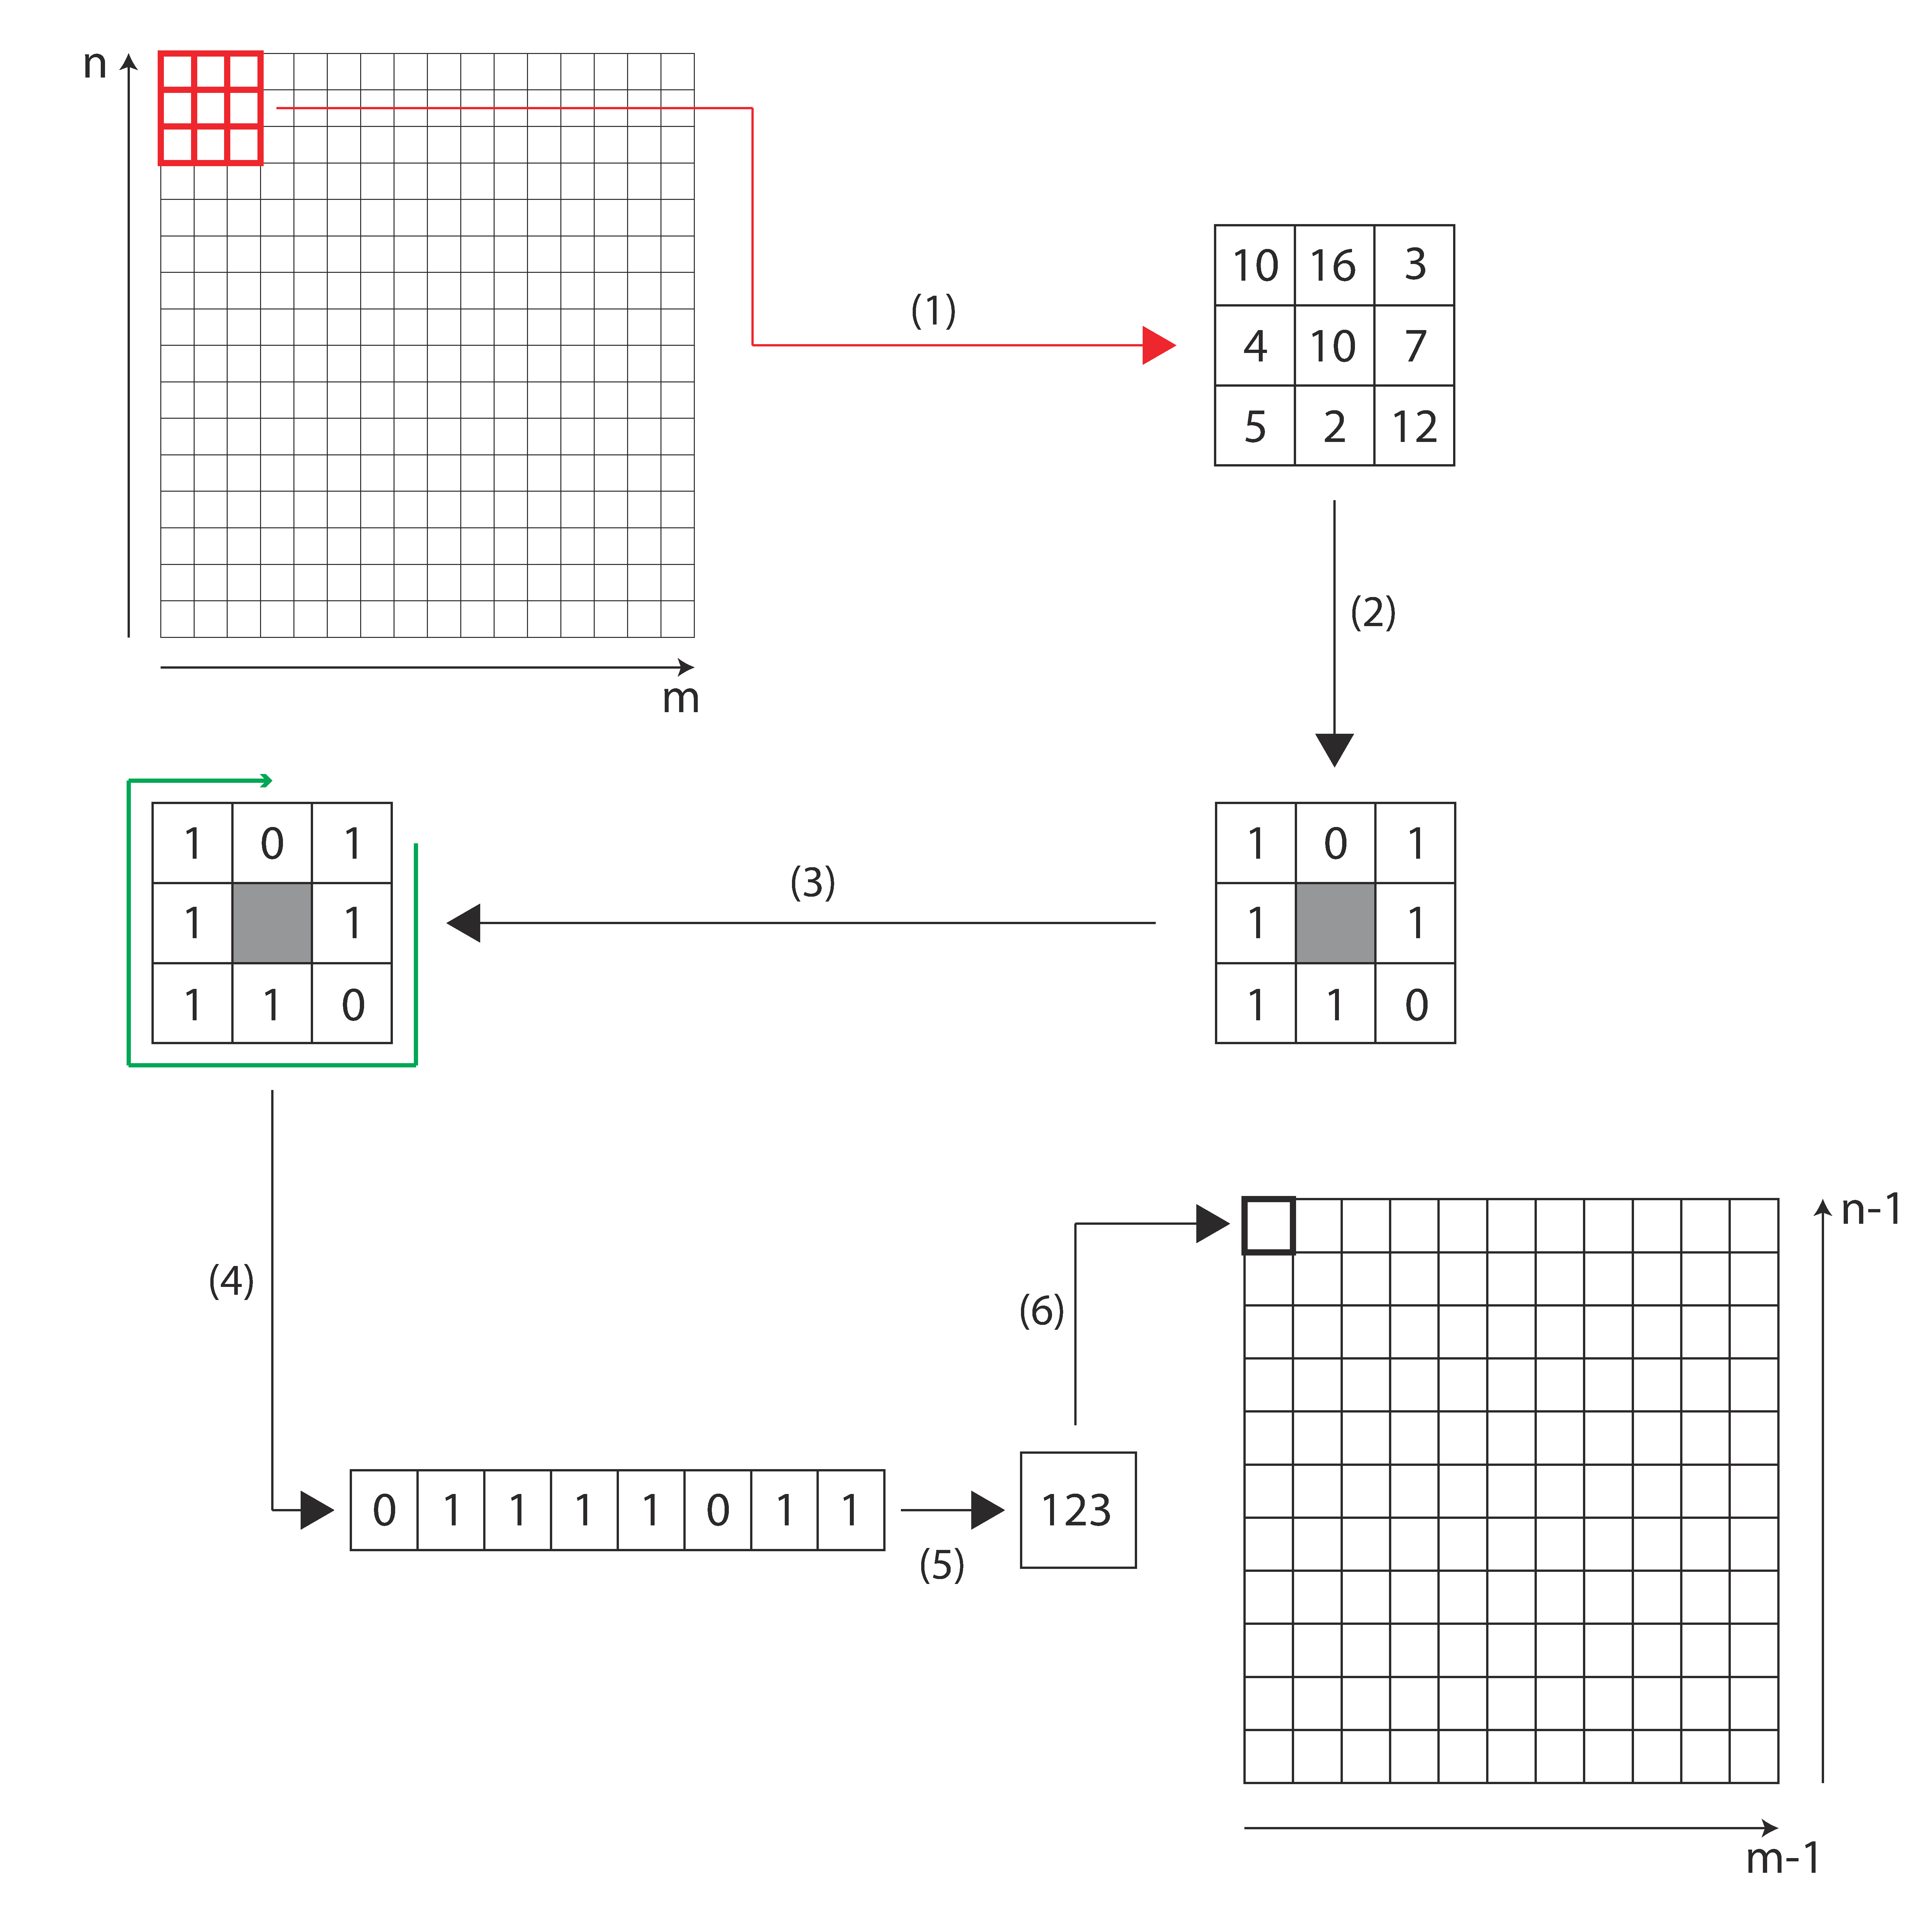
\includegraphics[width=\textwidth]{imagenes/marco_teorico/LBP/LBP_diagrama.pdf}
	\caption{Esquema método LBP}	
	\label{fig:LBP_diagrama}
\end{figure}

La figura \ref{fig:LBP_diagrama} muestra un esquematizado resumen del proceso de extración de características por este método.

La imagen original es tratada como una matriz de dimensiones $ n(filas) x\: m(columnas) $. A partir de esta, se extraen submatrices de dimensiones $3x3$ y se comienza el análisis de datos.

En la nueva submatriz, la posición central es comparada con las exteriores. Si, para una posición exterior, el valor central es menor o igual, se asigna a esta posición un valor 1. De ser mayor, se asigna un 0.

La nueva matriz binaria es tratada como un número binario de 8 dígitos, consisitiendo el siguiente paso en obtener el equivalente en base diez. Este último valor es almacenado en una nueva matriz de dimensiones $(n-1)x(m-1)$.

Realizando este proceso para toda la imagen original se tiene un conjunto de datos a partir de los cuales obtener el histograma sobre el que se basa el método \textbf{LBP}.

Teóricamente, el número máximo de características extraibles es 256 (ver \ref{eqn:LBP_rango}), pero pueden agruparse por rangos obteniendo grupos de características. Esta última opción es dependiente de la aplicación y del problema a tratar.

\begin{equation}
	[00000000, 11111111]_{2} \rightarrow [0, 255]_{10}
	\label{eqn:LBP_rango}
\end{equation}

\pagebreak
\subsection{Descriptores de Fourier}

Los descriptores de Fourier son un método de extracción de características por el cual un objeto bidimensional, cuyos puntos tienen las coordenadas $ (x_{k},\:y_{k})$, es mapeado a un dominio complejo de la forma $(x_{k},\:iy_{k})$. De tal forma, el objeto es tratado como una señal discreta compleja a la cual se aplica la transformada discreta de Fourier para encontrar sus armónicos (descriptores de Fourier).

La figura \ref{fig:fourier_poligono_trazo_continuo} representa una forma hexagonal rellena. Para obtener los descriptores de Fourier de este objeto, es necesario obtener el contorno exterior de la figura (véase \ref{fig:fourier_poligono_trazo_discontinuo}).

\begin{figure}[H]
	\centering
	\captionsetup{justification=centering}
	\begin{subfigure}{0.5\textwidth}
		\centering
		\captionsetup{justification=centering}
		
\includegraphics[width=0.5\textwidth]{imagenes/marco_teorico/Descriptores_Fourier/Poligono_trazo_continuo.pdf}	
		\caption{}
		\label{fig:fourier_poligono_trazo_continuo}
	\end{subfigure}
	\hfill
	\begin{subfigure}{0.7\textwidth}
		\centering
		\captionsetup{justification=centering}
		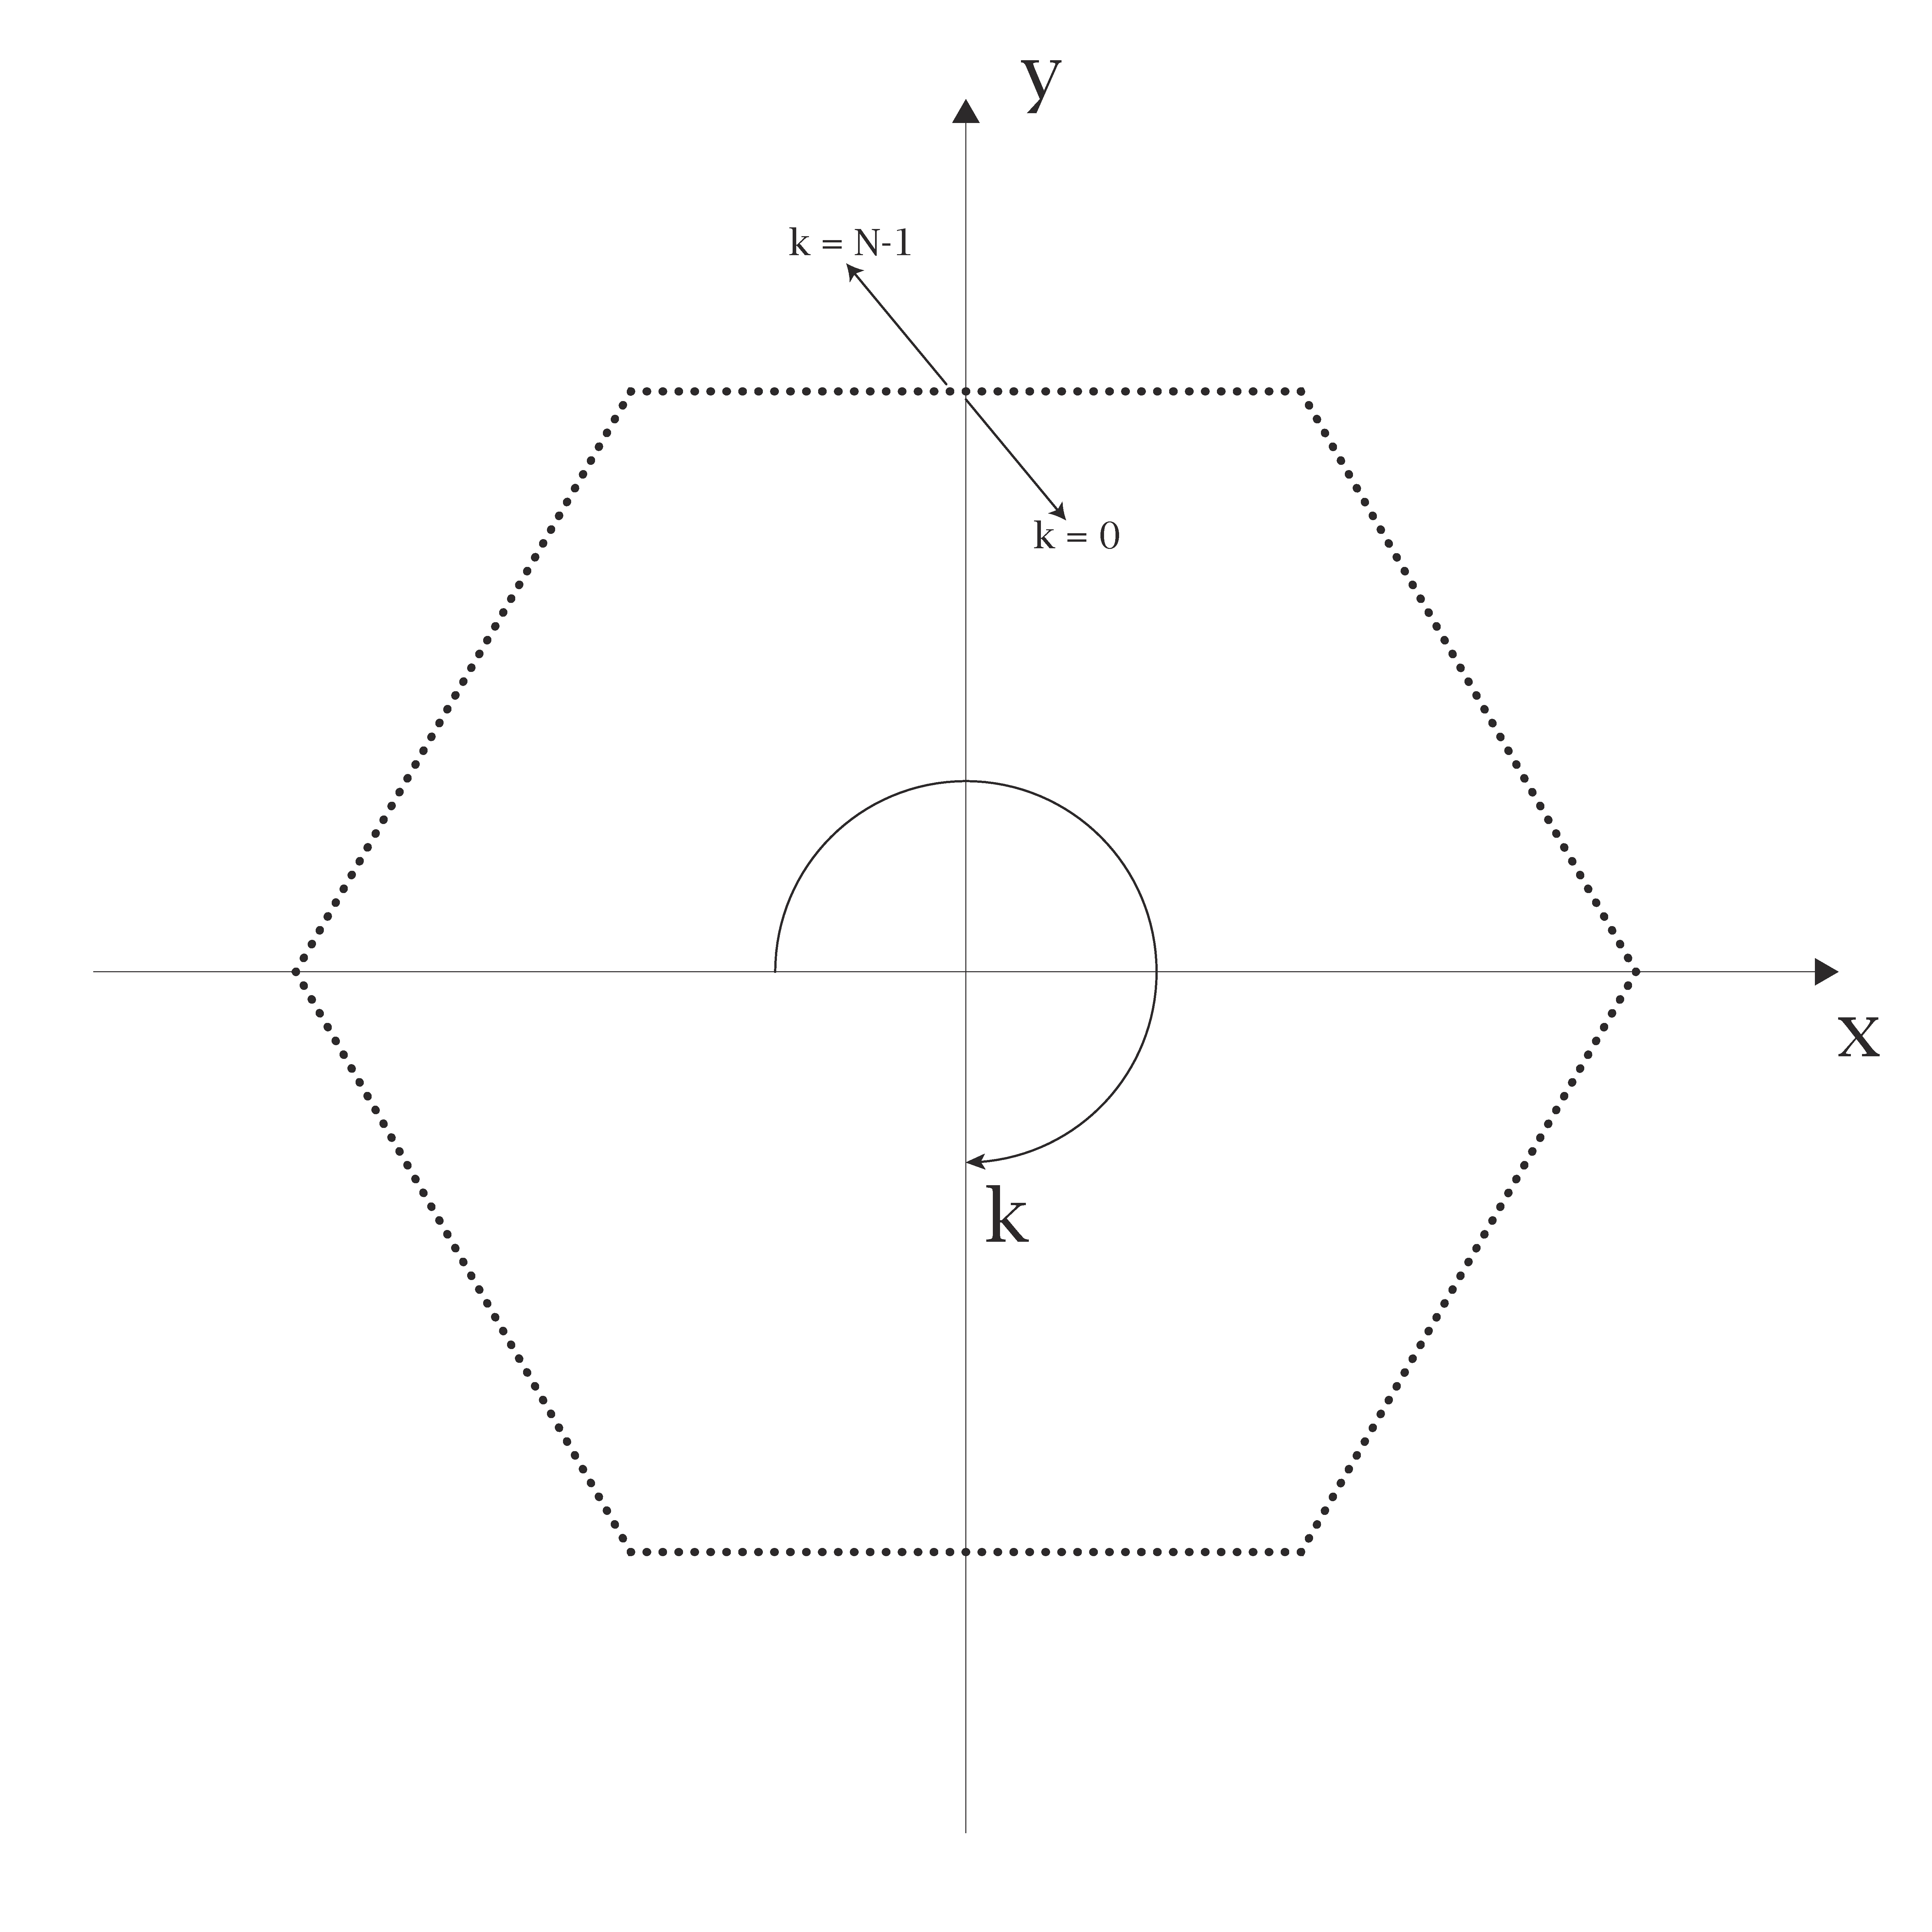
\includegraphics[width=0.7\textwidth]{imagenes/marco_teorico/Descriptores_Fourier/Poligono_ejesXY_k_figura.pdf}	
		\caption{}
		\label{fig:fourier_poligono_trazo_discontinuo}
	\end{subfigure}	
	\caption{Descriptores de Fourier}
	\label{fig:fourier_esquema}
\end{figure}

Este nuevo contorno está representado por $N$ puntos, de tal forma que cada punto puede definirse de la forma $ (x_{k},\:y_{k}),\:con\:k = 0, 1, 2, ..., N-1 $ y el contorno, a su vez, como la señal $f_{k} = (x_{k},\:y_{k})$.

Si $f_{k}$ es transformada al dominio complejo de la forma $f_{k} = x_{k} + iy_{k}$, es posible aplicar la transformada discreta de Fourier a $f_{k}$ para obtener los $N$ armónicos de la señal (descriptores de Fourier): 

\begin{equation}
	F_{m} = \sum_{k=0}^{N-1} f_{k}\cdot e^{-\dfrac{2\pi i}{N}mk},\qquad m = 0, 1, 2, ..., N-1
	\label{eqn:dft}
\end{equation}

La ecuación \ref{eqn:dft} (transformada discreta de Fourier), proporciona la serie de valores $ F_{0}, F_{1}, F_{2}, ..., F_{N-1} $, a partir de los cuales se obtienen los descriptores de Fourier (valores absolutos) $\lvert F_{0}, F_{1}, F_{2}, ..., F_{N-1} \rvert$.

En función de la resolución de la imagen original y su definición, el número de puntos del contorno $N$ variará, obteniéndose una cantidad diferente para cada caso. Por ello, el número de descriptores de Fourier obtenibles de cada imagen no será el mismo. Es por esto que, generalmente, de los $N$ descriptores obtenidos para cada imagen, se escogen solo $n\:|\:0\leq n\leq N$.

\begin{figure}[H]
	\centering
	\captionsetup{justification=centering}
	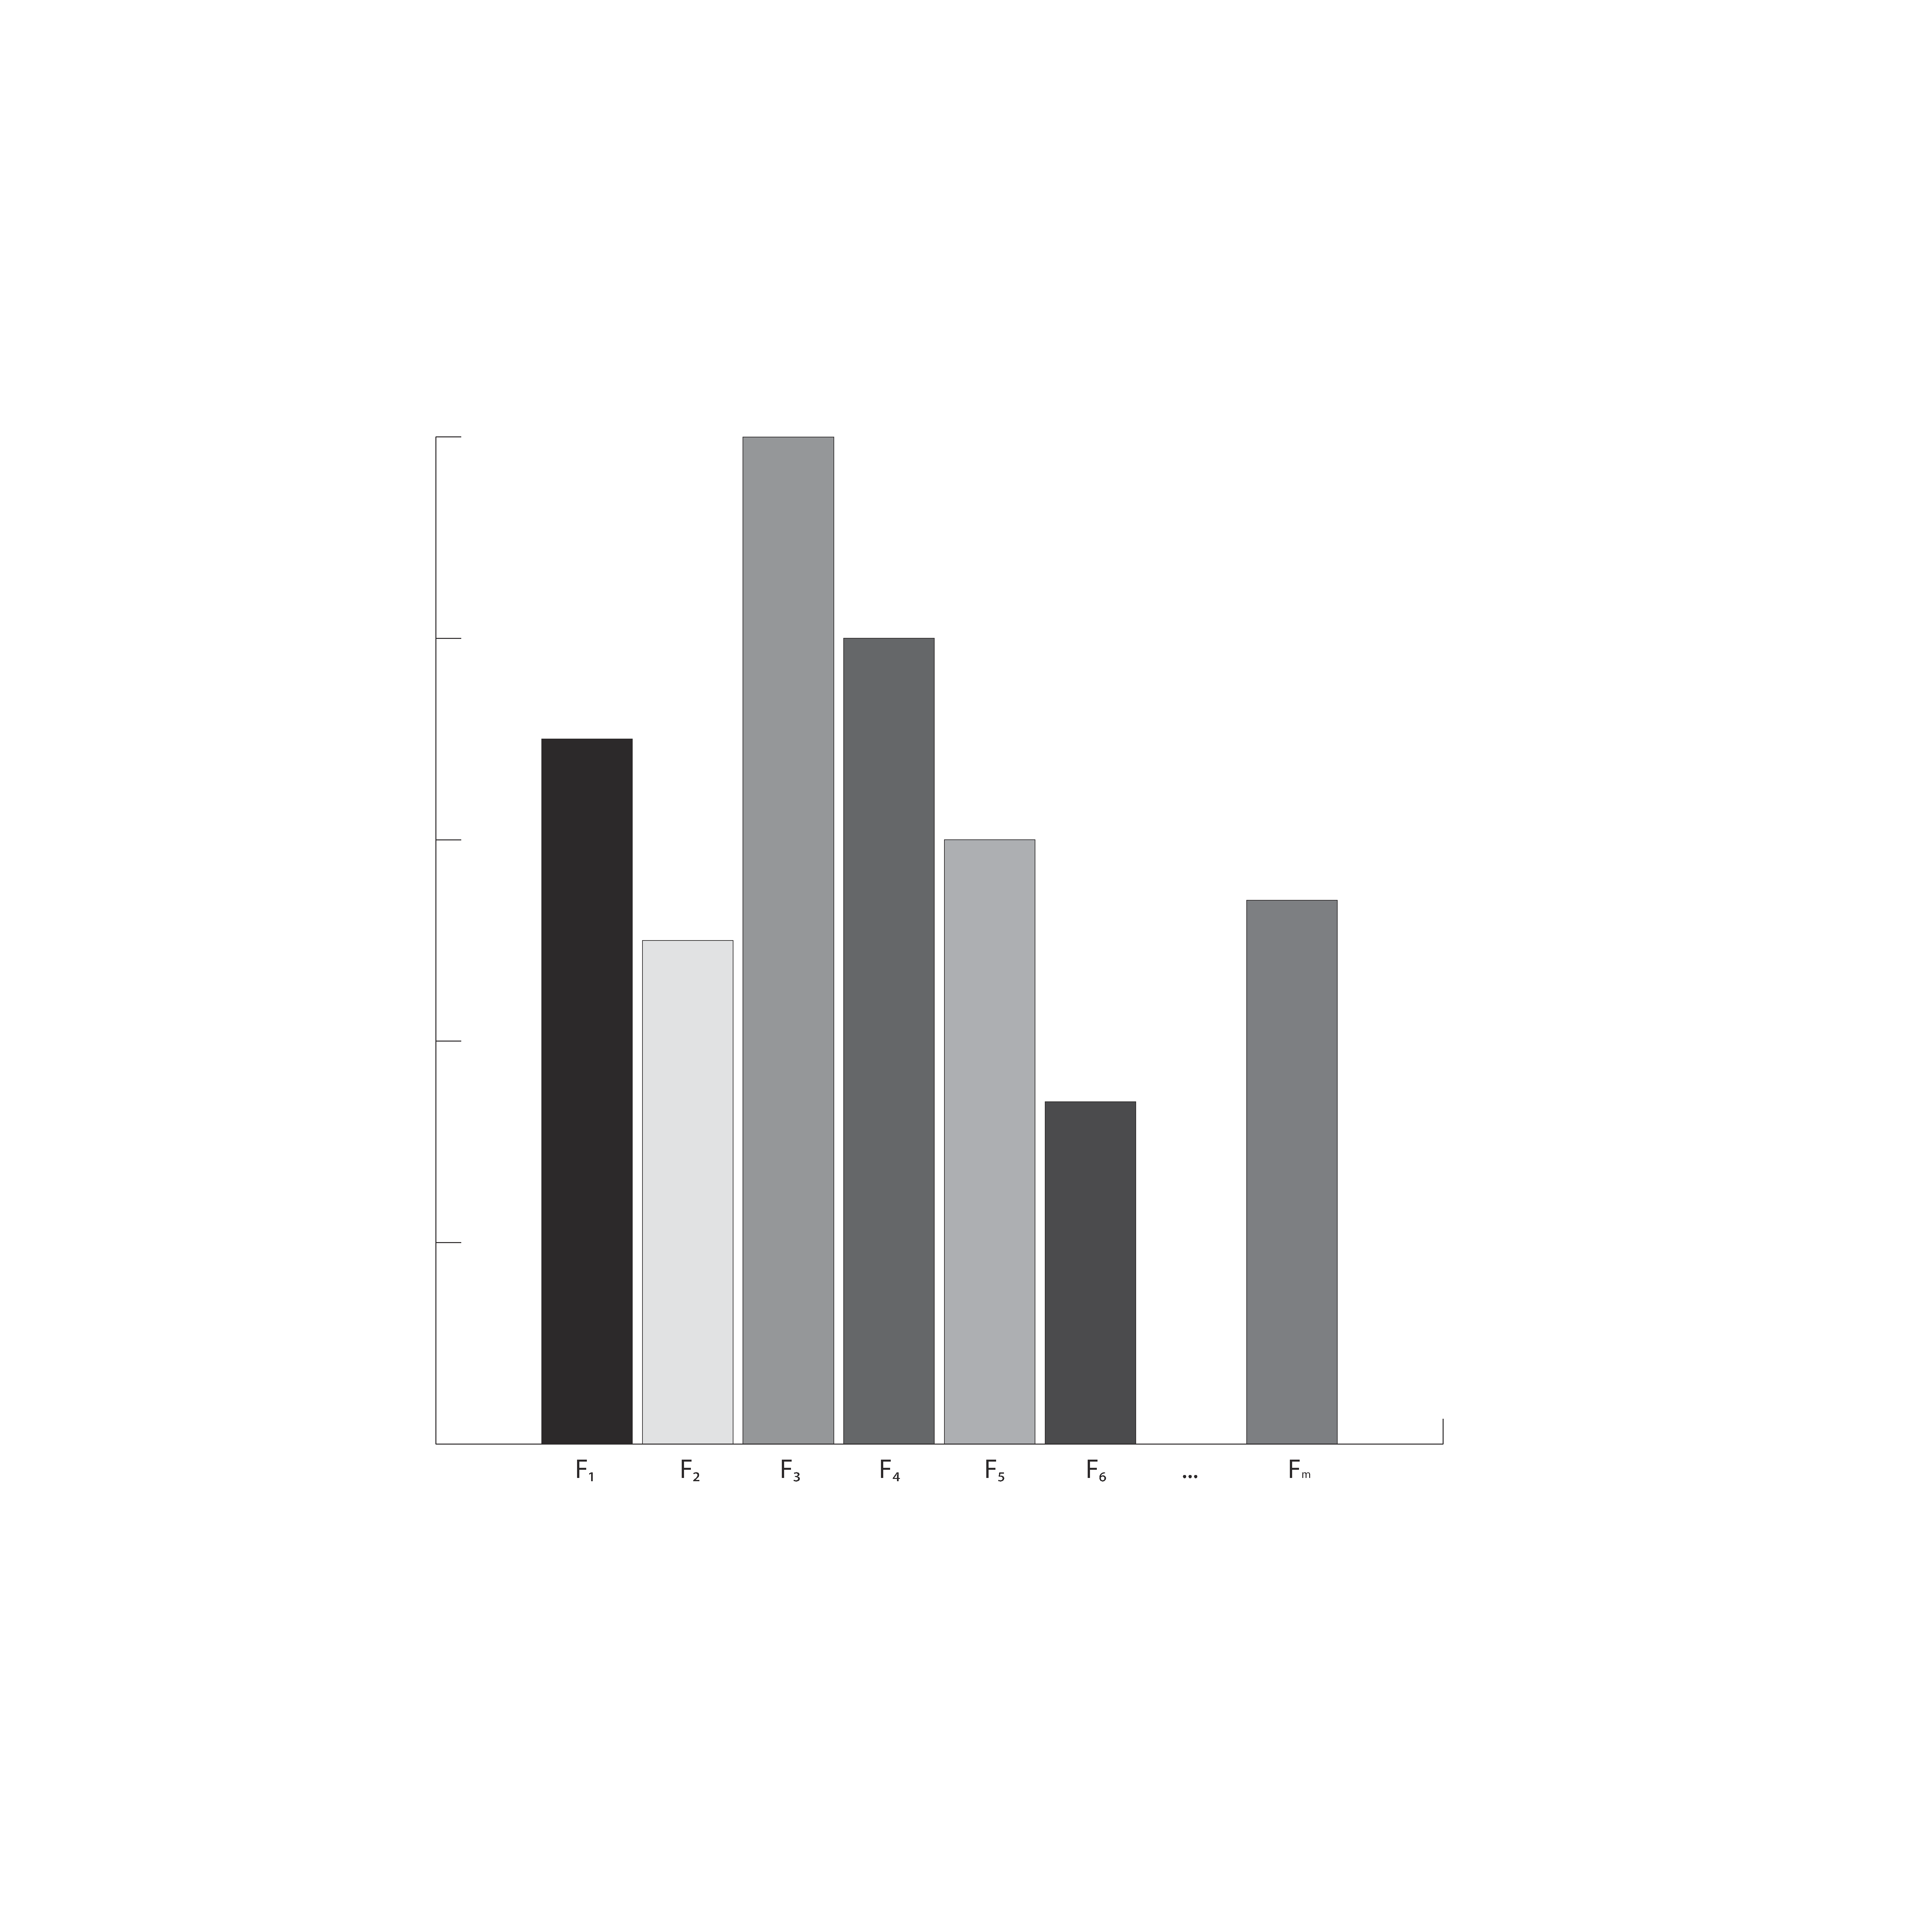
\includegraphics[width=\textwidth]{imagenes/marco_teorico/Descriptores_Fourier/Histograma_ejemplo_generico.pdf}
	\caption{}	
	\label{fig:fourier_histograma_generico_ejemplo}
\end{figure}

%% -----------------------------------------------------------------------%%

\section{Selección de características}

Una vez se han aplicado los métodos propuestos en la sección \ref{section:Extracción de catacterísticas}, es necesario realizar un análisis del poder clasificatorio de las características extraídas.

Para este trabajo, se han utilizado los siguientes métodos:
\begin{itemize}
	\item ANOVA
	\item SFS
\end{itemize}

\subsection{ANOVA}

\mynote{ANOVA es un conjunto de métodos estadísticos, entre los cuales está el F-Test, que es el que se usa aquí, principalmente.}

\mynote{Casi toda la información está sacada de \cite{frost_2020}.}

Conocido como Análisis de la Varianza (del inglés, \textit{ANalysis Of VAriance}).

Dado un ejemplo como una distribución de datos de dos clases (véase figura \ref{ANOVA:distribucion_ejemplo}), se disponen de dos características de clasificación: $(x,y)$.

\begin{figure}[h]
	\centering
	\captionsetup{justification=centering}
	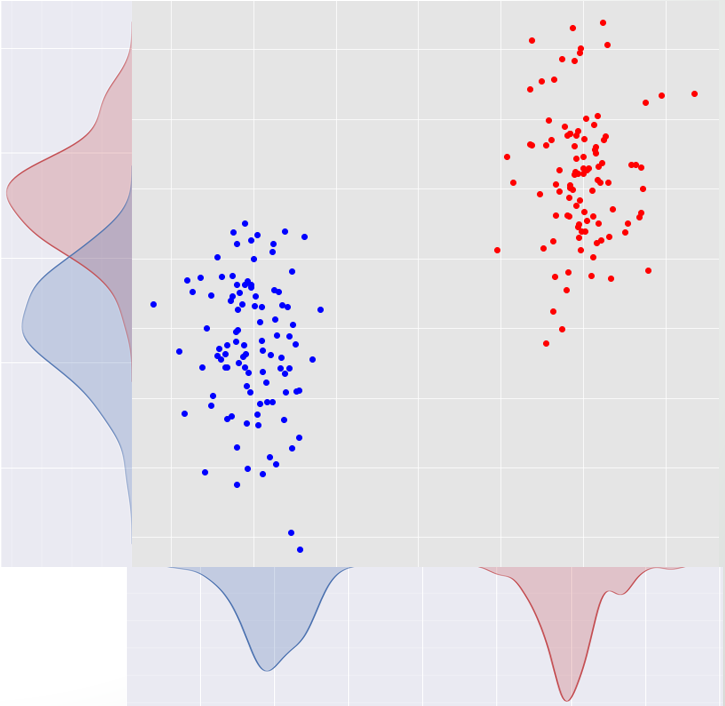
\includegraphics[scale = 0.5]{imagenes/marco_teorico/ANOVA/ejemplo_distribuciones.png}
	\caption{Distribuciones para un caso ejemplo de ANOVA}
	\label{ANOVA:distribucion_ejemplo}
\end{figure}

La característica $x$ es mucho mejor que la $y$ a simple vista pues, comparando las distribuciones de ambas, para $x$ se obtienen dos distribuciones claramente separadas por completo, mientras que para la característica $y$ las distribuciones se solapan.

También se puede comprobar que la distribución para la característica $x$ presenta una menor varianza (son más compactas) que con $y$.

Por tanto, para este ejemplo se puede definir la condición \ref{eqn:anova_1} como un parámetro de discriminación de características. Cuanto mayor sea para una característica, mejor será su poder de clasificación.

\begin{equation}
	F = \dfrac{Distancia\:entre\:clases}{Compacidad\:de\:clases}
	\label{eqn:anova_1}
\end{equation}

Matemáticamente, la fórmula \ref{eqn:anova_1} puede expresarse de la siguiente forma siguiendo el método ANOVA:

\begin{itemize}
	\item El numerador (distancia entre clases) es definible con:
	\begin{equation}
		n_{azul}(\overline{x_{azul}}-\overline{x})^{2} + n_{rojo}(\overline{x_{rojo}}-\overline{x})^{2}
	\end{equation}
	\item El denominador (compacidad de clases), que no es sino la varianza de clases, puede expresarse como:
	\begin{equation}
		\left(\dfrac{1}{(n_{azul}-1)+(n_{roja}-1)}\right)\left(\sum_{i=1}^{n_{azul}}\left(x_{i}-\overline{x_{azul}}\right)^{2}+\sum_{i=1}^{n_{roja}}\left(x_{i}-\overline{x_{roja}}\right)^{2}\right)
	\end{equation}
\end{itemize}

De tal forma, la ecuación \ref{eqn:anova_1} queda como:

\begin{equation}
	F = \dfrac{n_{azul}(\overline{x_{azul}}-\overline{x})^{2} + n_{rojo}(\overline{x_{rojo}}-\overline{x})^{2}}{\left(\dfrac{1}{(n_{azul}-1)+(n_{roja}-1)}\right)\left(\sum_{i=1}^{n_{azul}}\left(x_{i}-\overline{x_{azul}}\right)^{2}+\sum_{i=1}^{n_{roja}}\left(x_{i}-\overline{x_{roja}}\right)^{2}\right)}
	\label{eqn:ANOVA}
\end{equation}

La ecuación \ref{eqn:ANOVA} da un parámetro para una variable (en este caso $x$). En un problema con $k$ características, se obtendrían $k$ valores de $F$, es decir, una $F$ para cada variable.

Utilizando las $k$ características extraídas con los métodos propuestos en \ref{section:Extracción de catacterísticas}, ANOVA proporcionaría $F_{k}$ valores, de entre los cuales se seleccionarían los $N$ con mayor valor $F$. La ecuación \ref{eqn:ANOVA_F} define el valor de F para un caso con $j = 1,\:2,\:3,\:...,\:N$ clases. 

\begin{equation}
	F = \dfrac{\sum_{j=1}^{N} n_{j}\left(\overline{x_{i}}-\overline{x}\right)^{2}}{\left(\dfrac{1}{\sum_{j=1}^{N}(n_{j}-1)}\right) \left(\sum_{j=1}^{N}\left(\sum_{i=1}^{n_{j}}(x_{i}-\overline{x_{j}})^{2}\right)\right)}
	\label{eqn:ANOVA_F}
\end{equation}

\mynote{Este método solo da información sobre lo bien que UNA variable discrimina, pero no dice como de bien lo harían varias juntas.}

\subsection{SFS}

Los algoritmos SFS (del inglés \textit{Sequential Feature Selector} son un conjunto de técnicas de selección de caracteríticas (algoritmos voraces) usados para reducir un espacio incial n-dimensional de características a otro k-dimensional donde $k\leq d$.

Si se tiene el siguiente conjunto n-dimensional $Y = \{y_{1},y_{2},y_{3},...,y_{n}\}$ de características de entrada, utilizando un estimador determinado (SVM, Knn, SDG, etc.) y una métrica de rendimiento determinada, el algoritmo SFS busca obtener un conjunto de salida $X_{k} = \{x_{j} | j = 1,2,...,d;\: x_{j}\epsilon Y\},\: con \:k = (0,1,2,...,n)$ tal que $X_{k}$ esté formado por las $k$ características que maximicen la métrica.

Existen dos formas de realizar este proceso: hacia adelante (\textit{Forward}) y hacia detrás (\textit{Backwards}).

\begin{itemize}
	\item Sequential Forward Selection: se comienza con un conjunto vacío $X_{0} = \emptyset / k = 0$. En cada iteración se aumenta el número de características hasta encontrar la combinación que de el mejor resultado (según la métrica a resolver).
	\item Sequential Backward Selection: se comienza con el conjunto inicial $Y$. En cada iteración se disminuye el número de características hasta encontrar la combinación que de el mejor resultado (según la métrica a resolver).
\end{itemize}

Es posible no llegar al mismo resultado empleando sentidos contrarios y tampoco obtener el mismo resultado, en varias iteraciones, utilizando el mismo método.

\mynote{En \textit{Sklearn} la métrica para su modelo SFS es una evaluación de validación cruzada con un estimador definido en la llamada al método SFS.}

\newpage
\section{Métodos de evalución}

Antes de entrar en la sección de modelos de clasificación, es necesario definir las métricas propuestas utilizadas para analizar los resultados de los clasificadores.

En una primera instancia, es necesario presentar la \nameref{tab:matriz_confusion}.

\begin{table}[h]
	\centering
	\caption{Matriz de confusión}
	\label{tab:matriz_confusion}
	\begin{tabular}{cc|cc|}
		\cline{3-4}
		&  & \multicolumn{2}{c|}{Valor real} \\ \cline{3-4} 
		&  & \multicolumn{1}{c|}{1}    & 0   \\ \hline
		\multicolumn{1}{|c|}{Valor}    & 1 & \multicolumn{1}{c|}{True Positive (TP)}  & False Positive (FP) \\ \cline{2-4} 
		\multicolumn{1}{|c|}{predicho} & 0 & \multicolumn{1}{c|}{False Negative (FN)} & True Negative (TN)  \\ \hline
	\end{tabular}
\end{table}

La matriz de confusión es una herramienta muy utilizada para representar y ver de forma sencilla los resultados de una clasificación. En el caso de la tabla \ref{tab:matriz_confusion}, se representa una matriz de confusión para un caso de clasificación binaria, sin embargo puede utilizarse para casos multiclases.


\subsubsection{Curva ROC}

Lo habitual, además de deseable, a la hora de obtener los valores predichos de un clasificador, es hacerlo en forma de estimaciones probabilísticas en el rango $[0,\:1]$. De tal forma que, cuando se obtenga un valor, se puede comprobar con qué nivel de confianza el clasificador asigna a qué clase la muestra a predecir.

Muchas librerías de algoritormos supervisados devuelven los resultados, por defecto, como valores enteros $0$ o $1$, aplicando un umbral de clasificación de $0.5$. En el caso de obtener $0.5000001$ para la clase positiva y $0.4999999$ para la negativa, el clasificador asignaría automáticamente la muestra a la clase positiva, obviando el hecho de que realmente no existe un nivel de confianza suficiente para clasificar la muestra de tal forma.

Al obtenerse probabilidades y no valores discretos, para asignar clases, es necesario establecer un umbral de clasificación por el cual si $p(n) \geq umbral \rightarrow n = 1$. Por tanto, es conveniente encontrar un valor para el umbral de clasificación que haga que el clasificador funcione lo mejor posible.

Para cada valor de umbral se obtiene una matriz de confusión diferente, así como sus pertinentes métricas. Puede que exista un valor de umbral en el que el clasificador, para la base de datos dada, sea idóneo o puede que no existe ningún valor de umbral que haga que el clasificador discrimine correctamente. Sin embargo, es posible que, independientemente del umbral, el clasificador obtenga buenos resultados.

Para poder analizar estos casos, se recurre a la curva ROC (del inglés \textit{Receiver operating characteristic}).

La curva ROC es un gráfico utilizado para determinar la abilidad discriminante de un clasificador binario según su umbral de clasificación es variado.

Este gráfico se basa en el espacio ROC, que es básicamente la representación de la tasa de verdaderos positivos (o exhaustividad) (\ref{eqn:exhaustividad}) frente a la tasa de falsos positivos (\ref{eqn:fpr}).

\mynote{Exhaustividad: cantidad de valores reales positivos predichos como positivos.}

\begin{equation}
	Exhaustividad\:(TPR) = \dfrac{TP}{P} = \dfrac{TP}{TP+FN}
	\label{eqn:exhaustividad}
\end{equation}

\begin{equation}
	Tasa\: de\: falsos\: positivos\:(FPR) = \dfrac{FP}{N} = \dfrac{FP}{FP+TN}
	\label{eqn:fpr}
\end{equation}

\begin{figure}[h]
	\centering
	\captionsetup{justification=centering}
	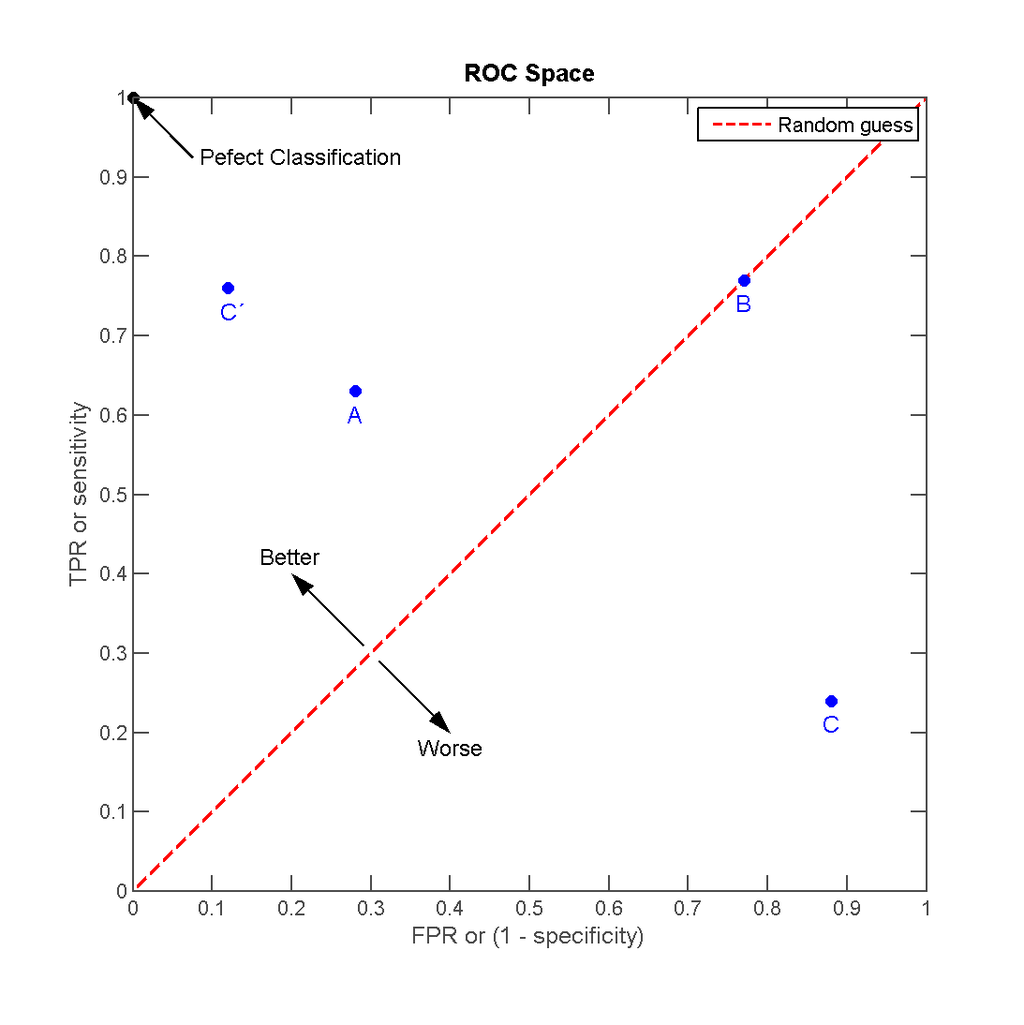
\includegraphics[width=0.5\textheight]{imagenes/marco_teorico/ROC/ROC_wiki.png}	
	\caption{Sacado de wikipedia (EDITAR)}
	\label{fig:roc_curva}
\end{figure}

La línea de puntos roja representa un clasificador puramente aleatorio que asigna un $0.5$ de probabilidades de pertencer a la clase positiva a cada muestra.

Para valores de umbral en el rango $[0,\:1]$, se obtienen los valores de \ref{eqn:exhaustividad} y \ref{eqn:fpr}, y se representa el punto correspondiente en el gráfico. De tal forma, se obtiene una curva escalonada que representa la calidad del clasificador.

El caso idóneo es aquel en el que la curva del clasificador es un escalón unidad, es decir, aquel clasificador que, para cualquier valor de umbral, se obtiene un 100\% de exhaustividad. Númericamente, este tipo de curva corresponde a una curva con una área bajo la curva de la unidad.

El peor caso es el clasificador cuya curva sea la inversa al escalón unidad pues, se obtiene un 0\% de exhaustividad para cualquier umbral, es decir, aquella curva con una área bajo la curva nula.

Por tanto, se define el parámetro \textbf{AUC}, del inglés \textit{Area Under the Curve}, que determina la calidad discriminante del clasificador. Cuanto mayor sea el valor de AUC, mejor el clasificador.

Sin embargo, la curva ROC no es correcta para casos desbalanceados ya que no representa correctamente los resultados, siendo necesario sustituirla por una curva de precisión-exhaustividad, que si lo hace \cite{10.1371/journal.pone.0118432}.

%\subsubsection{Métricas de rendimiento}
%
%A partir de la matriz de confusión se obtienen las llamadas métricas de rendimiento. Estos parámetros son utilizados en sistemas de clasificación, reconocimiento de patrones, etc, para analizar los resultados de dichos modelos.
%
%%\begin{itemize}
%%	\item Sensitividad, exhaustividad, tasa de positivos verdaderos: cantidad de valores reales positivos predichos como positivos.
%%		\begin{equation}
%%			Exhaustividad = \dfrac{TP}{P} = \dfrac{TP}{TP+FN}
%%			\label{eqn:exhaustividad}
%%		\end{equation}
%%	\item Exactitud: cantidad de predicciones que el modelo acertó.
%%		\begin{equation}
%%			Exactitud = \dfrac{TP+TN}{P+N} = \dfrac{TP+TN}{TP+TN+FP+FN}
%%			\label{eqn:exactitud}
%%		\end{equation}
%%	\item Precisión: cantidad de predicciones positivas acertadas correctamente.
%%		\begin{equation}
%%			Precision = \dfrac{TP}{TP+FP}
%%			\label{eqn:precision}
%%		\end{equation}
%%\end{itemize}
%
%Como se presenta en \cite{10.1371/journal.pone.0118432}, no todas las métricas de rendimiento son correctas para cualquier caso de clasificación, viéndose afectadas para casos desbalanceados.
%
%\mynote{Un caso desbalacenado de clasificación, binario o multiclase, es aquel donde la frecuencia de muestras de cada clase no es similar al del resto de clases. Es decir, para un caso binario, lo más común es tener muchas más muestras de la clase negativa (0) que de la positiva (1).}
%
%La imagen \ref{fig:comparacion_metricas} presenta la diferencia entre métricas para un caso desbalanceado respecto a un balanceado.
%
%\begin{figure}[h]
%	\centering
%	\captionsetup{justification=centering}
%	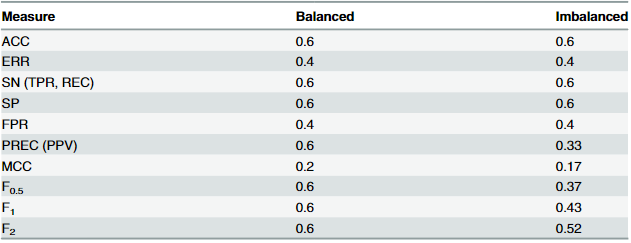
\includegraphics{imagenes/marco_teorico/Metricas/Tabla_articulo.png}
%	\caption{Métricas para caso balanceado y caso desbalanceado \cite{10.1371/journal.pone.0118432}}
%	\label{fig:comparacion_metricas}
%\end{figure}
%
%Muchas de las métricas mas usadas, como exactitud, tasa de falsos positivos o el error, no muestran diferencias entre casos.
%
%
%


\chapter{Metodología}

El proceso completo de clasificación puede dividirse en dos fases:

\subsubsection{Primera fase, extracción y selección de características}

\begin{figure}[H]
	\centering
	\captionsetup{justification=centering}
	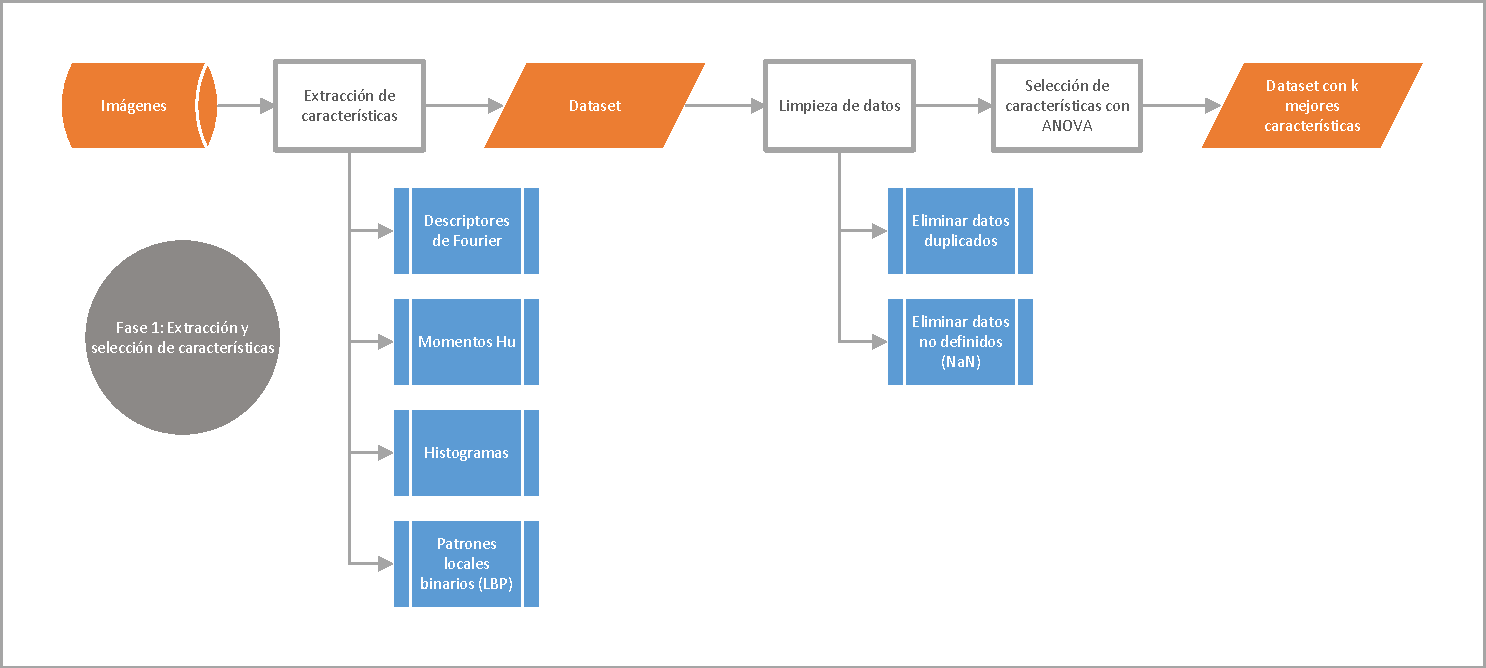
\includegraphics[width=\textwidth]{imagenes/metodología/Fase1.pdf}
	\caption{Procesos en la fase de extracción y selección de características}
	\label{met:fase1}
\end{figure}

\paragraph{Extracción de características}

El problema parte de un conjunto de imágenes almacenadas por clases y área a las que pertenecen. A partir de estas, se aplican los métodos de extracción de características. 

En el caso de extracción de Momentos Hu se ha hecho uso de la librería OpenCV, que implementa un algoritmo para extraer siete momentos Hu de una imagen binaria. 
La extracción de los histogramas de gradientes se ha realizado a partir de código propio. Los patrones locales binarios han sido implementados de igual forma con código propio. Los descriptores de Fourier han sido obtenidos haciendo uso de la librería \cite{Pybalu} para \textit{Python}, creada por Domingo Mery.

\mynote{No sé si puedo mostrarlo, pero realmente no es nada del otro mundo el código, solo unas pocas funciones no muy eficientes XD.}

De cada imagen se obtiene un vector de treinta y una posiciones (LBP ha sido descartado por no obtenerse un número uniforme de características, ya que estas dependen de la resolución de la imagen). Con un total de $n$ instancias (ó imágenes) se crea una matriz de dimensiones $nx31$, llamada $X$. Dado que los algoritmos de clasificación son supervisados, se crea, además, una matriz de etiquetas de valores $0,1,2,...,N$, siendo $N$ el número de clases, de tamaño $nx1$, llamada $Y$. Uniendo ambas matrices se obtiene el dataset.

\mynote{Normalmente un dataset se guarda como un diccionario, u objeto \textit{Bunch} de Sklearn\cite{scikit-learn}, donde sus llaves son las etiquetas, datos, datos de fourier, datos de HoG y datos de momentos, de tal forma que se puede guardar en memoria y cargarlo en cualquier momento.}

\paragraph{Limpieza de datos}

Con el dataset ya creado, es necesario entrar el proceso de limpieza de datos, que corresponde a dos subprocesos (para este caso):

\begin{itemize}
	\item Eliminación de datos duplicados: existe la posibilidad de que en el directorio de almacenamiento de imágenes exista la misma imagen duplicada varias veces, obteniéndose datos redundantes en el dataset, para ello, es necesario eliminar esos datos duplicados, dejando claro está al menos una muestra original.
	\item Eliminación de datos no definidos: En la obtención de momentos, al aplicar el escalado logarítmico es posible que algunos valores se devuelvan como indeterminados (por la naturaleza del logaritmo), de tal forma, se aplica la fórmula $Hu = -signo(Hu)log|Hu+10^{-12}|$ para obtener datos numéricos y no indeterminaciones.
\end{itemize}

\paragraph{Selección de características}

Con el dataset creado y corregido, se aplica el método de los valores F de ANOVA para obtener una descripción del poder discriminatorio de cada una de las 31 características del dataset. ANOVA se implementa a partir de la clase \textit{f\_classif} de Sklearn\cite{scikit-learn}, que devuelve un vector de tamaño $1x31$ con los 31 F valores de las características. Con la clase \textit{SelectKBest}, de Sklearn\cite{scikit-learn} también, se pueden seleccionar automáticamente, sin obtener previamente los F valores, las k mejores características en función de ANOVA.

Tras las selección de características, el dataset reduce su tamaño de $nx31$ a $nxk$.

\subsubsection{Segunda fase, selección y análisis del clasificador}

\begin{figure}[H]
	\centering
	\captionsetup{justification=centering}
	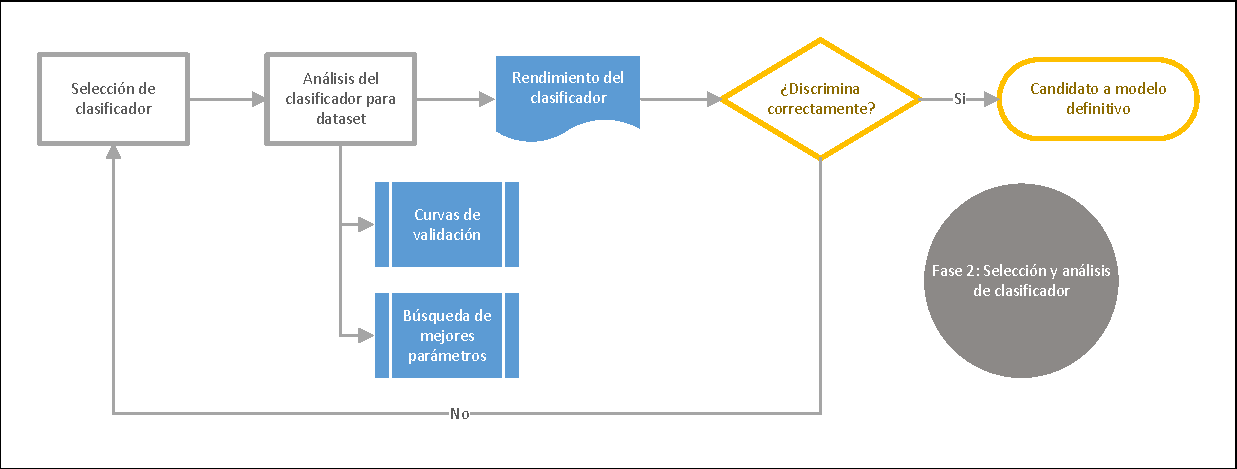
\includegraphics[width=\textwidth]{imagenes/metodología/Fase2.pdf}
	\caption{Selección y análisis del clasificador}
	\label{met:fase2}
\end{figure}

Con el dataset ya creado y las k mejores características seleccionadas se procede a realizar pruebas con diferentes clasificadores.

En primer lugar, es necesario comprobar si el dataset contiene un número balanceado de muestras, para así, poder determinar que métricas utilizar para analizar el rendimiento. 

Con un clasificador elegido para analizar su rendimiento (todos son clases de Sklearn \cite{sklearn_api}), se analiza el rendimiento del clasificador para el dataset en función de los valores de sus parámetros (curva de validación). Con este paso se consigue extraer un rango de valores para cada parámetro en el que el clasificador sobre ajuste una mínima cantidad, o discrimine perfectamente, con el cual hacer una búsqueda de los parámetros que devuelvan el mayor rendimiento para el clasificador elegido en el dataset.

Una vez obtenidos los mejores parámetros, se obtienen las métricas promedio de rendimiento (ya que es un problema multiclase) para el clasificador con esas variables. 

Si se considera que el clasificador realiza una buena discriminación, se plantea como buen candidato a modelo definitivo. De lo contrario, se escoge otro modelo de clasificador y se realiza de nuevo el mismo proceso.

%
%En este capítulo se presentan los procedimientos y técnicas empleadas para implementar y desarrollar los conceptos explicador en el capítulo \nameref{cap:marco_teorico}.
%
%El modo de funcionamiento ha consistido en implementar manualmente aquellos métodos que no pudieran obtenerse mediante librerías ya existentes. Para el resto, se ha hecho uso de las librerías de Sklearn, Numpy, OpenCV y Pybalu.
%
%\section{Implementación de los métodos de extracción de características}
%
%\paragraph{Preprocesado de imágenes} Para la tarea de lectura de imágenes, se ha hecho uso de la librería OpenCV de la siguiente forma:
%\begin{lstlisting}[language=python]	
%	img = cv2.imread(ruta+archivos)
%	img = cv2.normalize(img, 0, 255, cv2.NORM_MINMAX)    
%	gris = cv2.cvtColor(img,cv2.COLOR_BGR2GRAY)        
%	_,th = cv2.threshold(gris,0,255,cv2.THRESH_BINARY+cv2.THRESH_OTSU)	
%\end{lstlisting}
%
%La primera linea hace uso de la función \textit{imread} para leer la imagen como una matriz $\mbox{img}$. A continuación, se le aplica una normalización $\mbox{MINMAX}$, donde al mínimo valor de la imagen se le asigna el valor 0, al máximo 255, con el resto de valores siendo escalados proporcionalmente.
%
%Para los métodos que requieren imágenes binarias, las líneas 3 y 4 se utilizan para convertir la imagen de espacio RGB a escala de grises (línea 3) con la función \textit{cvtColor} y, a continuación, se implementa la función \textit{threshold} para convertir la imagen en escala de grises a binaria, según un umbral definido por un método automático (\textit{THRESH-OTSU}).
%
%Para los métodos que no requieren de una imagen binaria, las lineas 3 y 4 no son añadidas.
%
%\subsection{Momentos de imagen}
%Han sido implementados haciendo uso de la librería OpenCV (a partir de una imagen binaria):
%
%\begin{lstlisting}[language=python]	
%	momentos = cv2.moments(th)
%	hu = cv2.HuMoments(momentos)
%	for i in range(len(hu)):
%		hu[i] = -np.sign(hu[i])*np.log10(np.abs(hu[i])+1e-20)   
%\end{lstlisting}
%
%Las líneas 1 y 2 devuelven los momentos centralizados y de Hu, respectivamente. Las líneas 6 y 7 son añadidas para convertir los momentos obtenidos a una escala logarítima de más fácil comparación según la fórmula \ref{hu:escalado}. El coeficiente $1^{-20}$ es añadido para evitar que la fórmula devuelva $NaN$.
%
%\begin{equation}
%	Hu = -sgn(hu)\log\lvert Hu+1^{-20}\rvert
%	\label{hu:escalado}
%\end{equation}
%
%De esta forma presentada, para una imagen, se obtiene un vector de siete elementos con los siete momentos de Hu.
%
%\subsection{Descriptores de Fourier}
%
%Para esta tarea se ha hecho uso de la librería Pybalu\cite{Pybalu}, que implementa una función de obtención de los coeficientes de Fourier para una imagen binaria. Internamente la función está configurada para devolver los 16 primeros coeficientes. Se puede cambiar, pero véase \nameref{subsection:fourier}.
%
%\begin{lstlisting}[language=python]
%	th = (th ==255)*1
%	f = extract_features(['fourierdes'] ,bw = th)
%	f = f/np.linalg.norm(f)  
%\end{lstlisting}
%
%Al igual que con momentos, el método de los descriptores de Fourier requieren una imagen binaria. En este caso, la librería Pybalu interpreta una imagen binaria como una matriz de [0,1], por lo que requiere cambiar los valores en 255 por 1 (línea 1). La línea 2 hace una llamada a la función de extracción. La línea 3 implementa un normalizado euclidiano al vector de 16 posiciones f, para obtener un resultado comparable en todos los casos.
%
%\subsection{Histogramas de gradientes}
%
%\subsection{Patrones locales binarios}
%
%\section{Implementación de la selección de características}
%
%\subsection{SFS}
%
%El algoritmo SFS no ha sido implementado en el proceso, aún siendo un excelente método de selección de características por varias razones:
%
%\begin{itemize}
%	\item Requiere de un estimador previamente definido: SFS viene implementado como método de selección en Sklearn y Mlextend, pero ambas implementaciones requieren la definición de un modelo de clasificación previo sobre el cual basar las métricas de análisis para obtener las k mejores características. Dado que clasificadores como SVM pueden parametrizarse de muchas formas diferentes, SFS siempre devolverá un resultado diferente para cada modelo particular, por lo tanto, no se puede concluir con una selección objetiva e independiente del clasificador a seleccionar.
%	\item No devuelve los mismos resultados de la forma hacia delante frente hacia detrás.
%\end{itemize}
%
%\subsection{ANOVA}
%
%Anova, a diferencia de SFS, si devuelve información independiente del clasificador, por lo tanto, ha sido la opción elegida para la selección de características.
%
%Sklearn propociona una función para obtener los F-valores de las características de una forma muy sencilla:
%
%\begin{lstlisting}[language=python]
%	f = f_classif(X, y)
%\end{lstlisting}
%
%El método \textit{f\_classif} devuelve el vector f (F-valores) para determinar qué características escoger.
%
%\subsection{Modelos de clasificación}
%
%Para esta sección, se han utilizado por completo los clasificadores implementados en Sklearn.
%
%\subsubsection{Knn}
%
%Sklearn proporciona tanto el clasificador Knn genérico como la versión alternativa de k-centroides.
%
%\paragraph{Knn} class sklearn.neighbors.KNeighborsClassifier(n\_neighbors=k, *, weights='uniform', algorithm='auto', leaf\_size=30, p=2, metric='minkowski', metric\_params=None, n\_jobs=None)\cite{sklearn_api}
%
%\begin{itemize}
%	\item n\_neighors: nº de vecinos para determinar clasificación
%	\item weights: peso otorgado a cada muestra de entrenamiento para calcular distancias
%	\item Uniforme: todas las muestras tienen la misma influencia
%	\item Distancia: la influencia es inversa de la distancia. A mayor distancia, menos influye el punto en el resultado.
%	\item p: determina el tipo de distancia a usar (Manhattan o Euclidiana)
%	\item algorithm: sklearn determina en función del tipo de problema el mejor algortimo a usar
%\end{itemize}
%
%\paragraph{Centroide más cercano} \textit{class sklearn.neighbors.NearestCentroid(metric='euclidean')}\cite{sklearn_api}. Solo se ha de definir la distancia a usar para clasificar.
%
%\subsubsection{SVM}
%
%Sklearn proporciona tres clasificadores que siguen el planteamiento teórico de los SVM:
%
%\begin{itemize}
%	\item LinearSVC: implementación SVM de la librería liblinear que sólo permite la utilización de un kernel lineal. Está optimizado para problemas lineales y permite usar funciones de pérdida diferentes a la estándar \textit{hinge loss}.
%	\item SVC y NuSVC: implementaciones SVM de la librería libsvm. El primero utiliza el parámetro de regularización C y el segundo $\nu$.
%\end{itemize}
%
%\paragraph{LinearSVC}
%
%\section{Desarrollo}
%
%Se empieza con un directorio de carpetas de imágenes almacenadas por el área al que pertenecen en el HMI. Este conjunto de imágenes son extraídas y 


\chapter{Resultados}

\section{Problema desbalanceado}

Visualizando el número de muestras para tanto la clase B345 como C1C9 (figuras \ref{fig:frecuencia_dataset_b345} y \ref{fig:frecuencia_dataset_c1c9}, respectivamente y el número de muestras por clase en las tablas \ref{tab:n_muestras_b345} y \ref{tab:n_muestras_c1c9})se puede afirmar que se trata de un problema de clasificación desbalanceado.

\begin{figure}[H]
	\centering
	\captionsetup{justification=centering}
	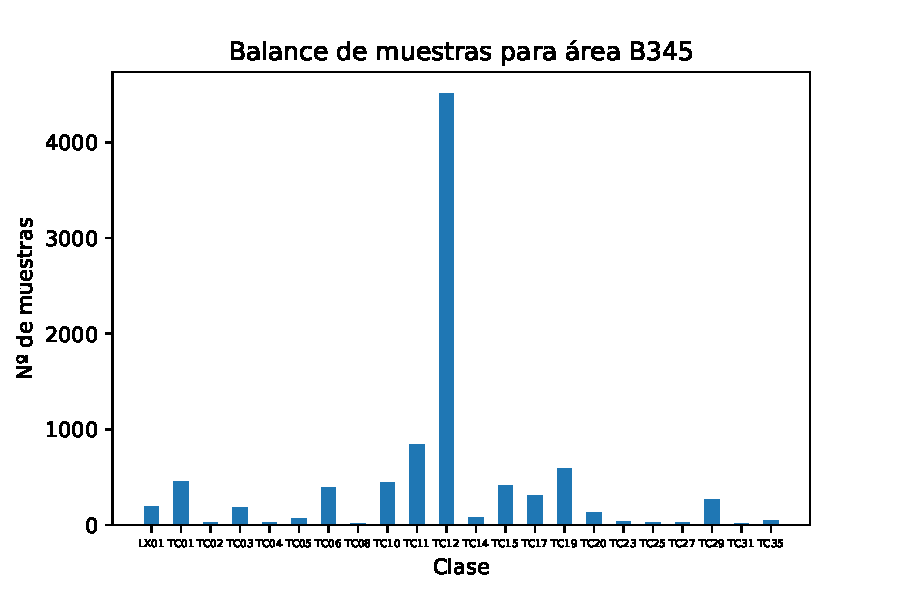
\includegraphics[width=\textwidth]{imagenes/resultados/balance/B345.pdf}
	\caption{Nº de muestras para el dataset del área B345}
	\label{fig:frecuencia_dataset_b345}
\end{figure}

\begin{table}[H]
	\centering
	\begin{tabular}{|c|c|}
		\hline
		Clase & Nº de muestras \\ \hline
		LX01 & 194 \\ \hline
		TC01 & 457 \\ \hline
		TC02 & 22 \\ \hline
		TC03 & 185 \\ \hline
		TC04 & 25 \\ \hline
		TC05 & 64 \\ \hline
		TC06 & 397 \\ \hline
		TC08 & 15 \\ \hline
		TC10 & 442 \\ \hline
		TC11 & 838 \\ \hline
		TC12 & 4511 \\ \hline
	\end{tabular}
	\begin{tabular}{|c|c|}
		\hline	
		TC14 & 82 \\ \hline
		TC15 & 414 \\ \hline
		TC17 & 304 \\ \hline
		TC19 & 590 \\ \hline
		TC20 & 131 \\ \hline
		TC23 & 38 \\ \hline
		TC25 & 30 \\ \hline
		TC27 & 21 \\ \hline
		TC29 & 269 \\ \hline
		TC31 & 18 \\ \hline
		TC35 & 52 \\ \hline
	\end{tabular}
	\caption{N$^\circ$ de muestras para área B345}	
	\label{tab:n_muestras_b345}
\end{table}

\begin{figure}[H]
	\centering
	\captionsetup{justification=centering}
	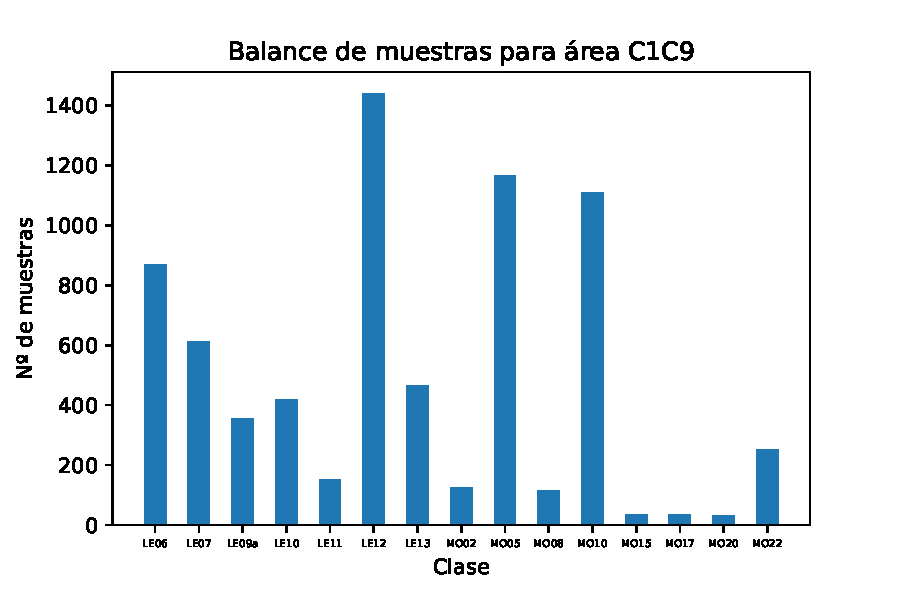
\includegraphics[width=\textwidth]{imagenes/resultados/balance/C1C9.pdf}
	\caption{Nº de muestras para el dataset del área C1C9}
	\label{fig:frecuencia_dataset_c1c9}
\end{figure}


\begin{table}[H]
	\centering
	\begin{tabular}{|c|c|}
		\hline
		Clase & Nº de muestras \\ \hline
		LE06 & 869 \\ \hline
		LE07 & 613 \\ \hline
		LE09a & 354 \\ \hline
		LE10 & 418 \\ \hline
		LE11 & 153 \\ \hline
		LE12 & 1440 \\ \hline
		LE13 & 464 \\ \hline
		MO02 & 124 \\ \hline
	\end{tabular}
	\begin{tabular}{|c|c|}
		\hline	
		MO05 & 1168 \\ \hline
		MO08 & 116 \\ \hline
		MO10 & 1109 \\ \hline
		MO15 & 35 \\ \hline
		MO17 & 34 \\ \hline
		MO20 & 31 \\ \hline
		MO22 & 253 \\ \hline
	\end{tabular}
	\caption{N$^\circ$ de muestras para área C1C9}	
	\label{tab:n_muestras_c1c9}
\end{table}

Para analizar resultados, al tratar con clases desbalanceadas, no se usa en ningún momento la exactitud y, a priori, tanto promedio micro, macro y ponderado de las métricas darán resultados que favorezcan a las clases más frecuentes.

\section{ANOVA}

El método LBP no ha sido utilizado debido a que el numero de características extraídas de una imagen depende de su resolución. Dado que el dataset contiene imágenes con resoluciones diferentes, no se puede obtener un número uniforme de características.

Para la selección de características con ANOVA, se obtienen los siguientes resultados:

\subsection{Área B345}

\begin{table}[H]
	\centering
	\begin{tabular}{|c|c|}
		\hline
		Característica & F-valor \\ \hline
		H0 & 23859.201619 \\ \hline
		H4 & 12429.265116 \\ \hline
		H6 & 7880.238366 \\ \hline
		M3 & 3895.946032 \\ \hline
		H1 & 3827.930644 \\ \hline
		M0 & 3486.251597 \\ \hline
		H5 & 3090.149390 \\ \hline
		M2 & 2880.764008 \\ \hline
		F7 & 2439.522794 \\ \hline
		F6 & 1810.805758 \\ \hline
		H2 & 1715.595292 \\ \hline
		F5 & 1267.176107 \\ \hline
		F4 & 1049.974086 \\ \hline
		M1 & 1003.760963 \\ \hline
		F2 & 879.120903 \\ \hline
	\end{tabular}
	\begin{tabular}{|c|c|}
		\hline
		F3 & 821.479145 \\ \hline
		F11 & 675.605577 \\ \hline
		F1 & 670.737686 \\ \hline
		F0 & 661.628967 \\ \hline
		M4 & 514.887416 \\ \hline
		F9 & 472.654444 \\ \hline
		M5 & 386.561602 \\ \hline
		F12 & 369.108364 \\ \hline
		M6 & 202.739105 \\ \hline
		F8 & 202.675900 \\ \hline
		F14 & 172.541408 \\ \hline
		F10 & 144.443042 \\ \hline
		F15 & 86.515230 \\ \hline
		F13 & 77.369423 \\ \hline
		H3 & nan \\ \hline
		H7 & nan \\ \hline
	\end{tabular}	
	\caption{Resultados ANOVA para área B345}	
	\label{tab:anova_b345}
\end{table}

\begin{figure}[H]
	\centering
	\captionsetup{justification=centering}
	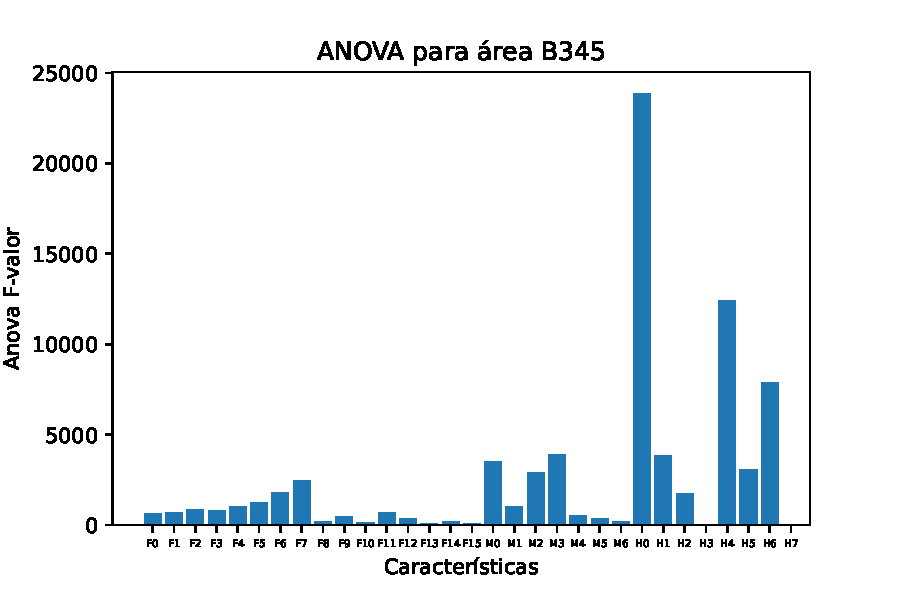
\includegraphics[width=\textwidth]{imagenes/resultados/anova/ANOVA_b345.pdf}
	\caption{Resultados ANOVA para área B345}
\end{figure}

De entre todas las características extraídas, por el método ANOVA se ha determinado que H0, H1, H4, H5, H6 y F7 son las seis características más discriminantes, seguidas por los momentos M0, M1, M2 y M3.

En el caso de H3 y H7, ANOVA devuelve un valor no definido pues, estas características son constantes para todas las muestras.

\subsection{Área C1C9}

\begin{table}[H]
	\begin{tabular}{|c|c|}
		\hline
		Característica & F-valor \\ \hline
		M1 & 6125.638894 \\ \hline
		H4 & 5857.112939 \\ \hline
		H0 & 4554.790583 \\ \hline
		M0 & 3048.724574 \\ \hline
		H5 & 1787.841543 \\ \hline
		M2 & 1752.153444 \\ \hline
		H2 & 1427.452251 \\ \hline
		H1 & 1040.217828 \\ \hline
		M3 & 817.966512 \\ \hline
		F3 & 528.279034 \\ \hline
		H6 & 376.474004 \\ \hline
		F7 & 276.076666 \\ \hline
		F1 & 267.434392 \\ \hline
		F10 & 252.051888 \\ \hline
		M5 & 229.500016 \\ \hline
	\end{tabular}	
	\begin{tabular}{|c|c|}
		\hline
		F6 & 221.004593 \\ \hline
		F5 & 189.035358 \\ \hline
		F8 & 164.096954 \\ \hline
		F14 & 156.956539 \\ \hline
		M4 & 140.206197 \\ \hline
		F2 & 133.046369 \\ \hline
		F9 & 122.262756 \\ \hline
		F11 & 105.074395 \\ \hline
		F0 & 78.174618 \\ \hline
		F4 & 77.091309 \\ \hline
		M6 & 75.595968 \\ \hline
		F15 & 73.126625 \\ \hline
		F12 & 60.370951 \\ \hline
		F13 & 48.366221 \\ \hline
		H3 & nan \\ \hline
		H7 & nan \\ \hline
	\end{tabular}	
	\caption{Resultados ANOVA para área C1C9}
	\label{tab:anova_c1c9}
\end{table}

\begin{figure}[H]
	\centering
	\captionsetup{justification=centering}
	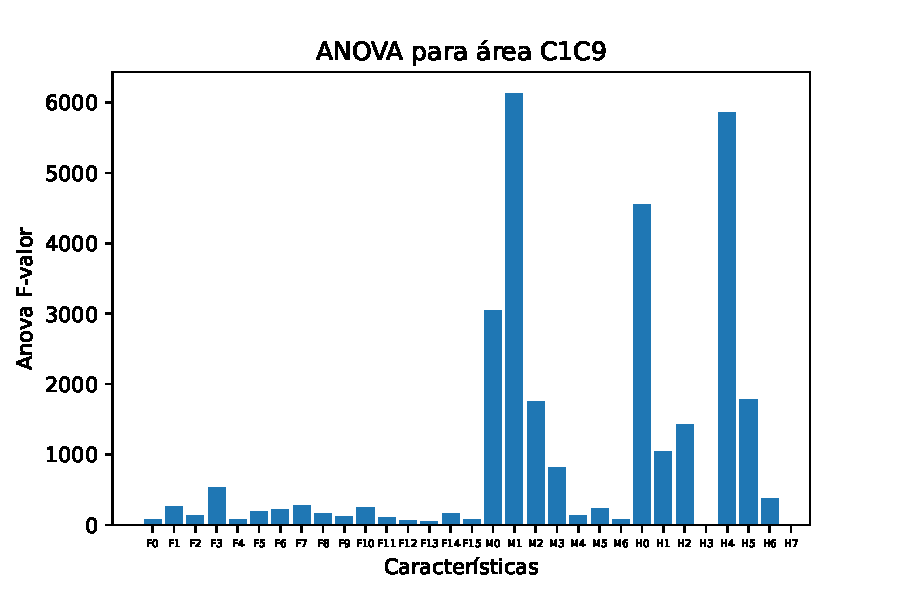
\includegraphics[width=\textwidth]{imagenes/resultados/anova/ANOVA_C1C9.pdf}
	\caption{Resultados ANOVA para área C1C9}
\end{figure}

Al igual que en el área B345, las características de Hog siguen siendo significativas, pero en este caso el momento de Hu segundo (M1) es la segunda característica más significativa.

Igual que para B345, H3 y H7 no están definidas ($NaN$) por ser constantes.

\mynote{Usando la clase \textit{SelectKBest}, proporcionada por Sklearn, se pueden escoger automáticamente las k mejores características según los F-valores de ANOVA.}

\section{K-vecinos más cercanos}

Al no devolver Knn predicciones probabilísticas, no se usa la curva ROC ó Precisión-Exhaustividad para analizar sus resultados.

\subsection{Resultados con clasificador Knn para área B345}

\subsubsection{Curvas de validación para Knn}

A continuación, se presenta la curva de validación para ambos modelos de clasificador Knn (uniforme y distancia) para las métricas de recall, precisión y $f_{1}$. 

Para todos los resultados, se han seleccionado las siete mejores características según ANOVA (véase \ref{tab:anova_b345}).

\begin{figure}[H]
	\centering
	\captionsetup{justification=centering}
	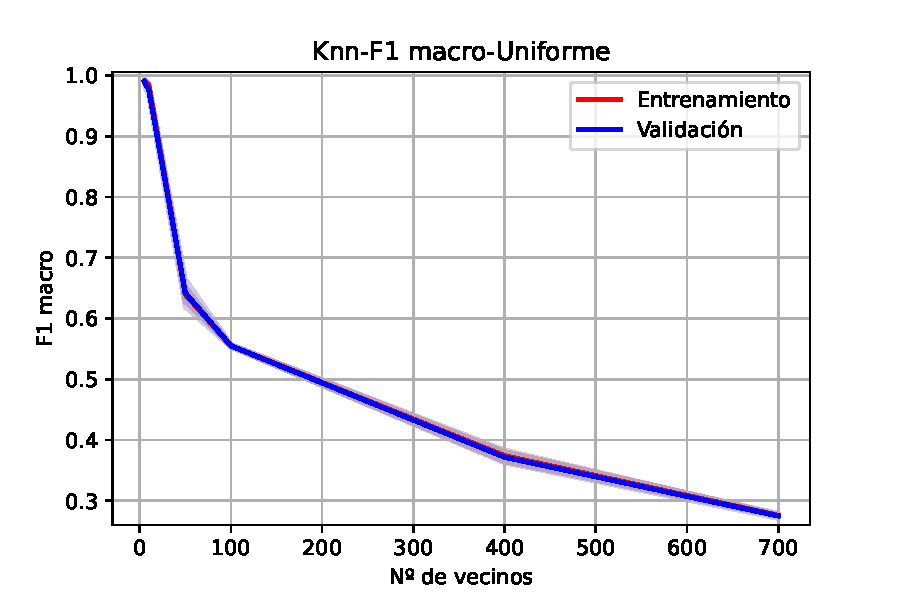
\includegraphics[width=\textwidth]{imagenes/resultados/curvas_validación/Knn-F1 macro-Uniforme.pdf}
	\caption{Curva de validación para modelo KNN uniforme, F1 macro}
	\label{fig:res_knn_vc_f1}
\end{figure}

\begin{figure}[H]
	\centering
	\captionsetup{justification=centering}
	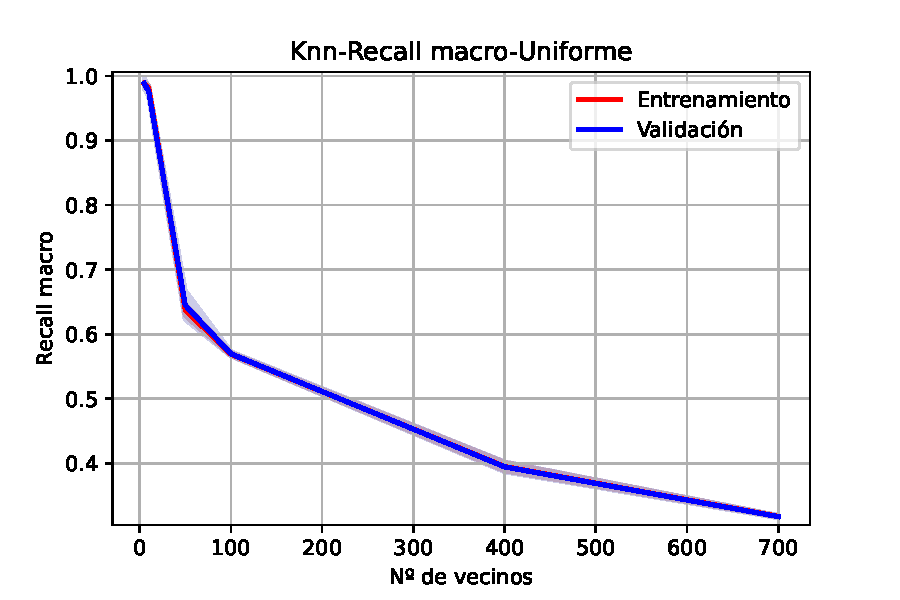
\includegraphics[width=\textwidth]{imagenes/resultados/curvas_validación/Knn-Recall macro-Uniforme.pdf}
	\caption{Curva de validación para modelo KNN uniforme, Recall macro}
	\label{fig:res_knn_vc_recall}
\end{figure}

\begin{figure}[H]
	\centering
	\captionsetup{justification=centering}
	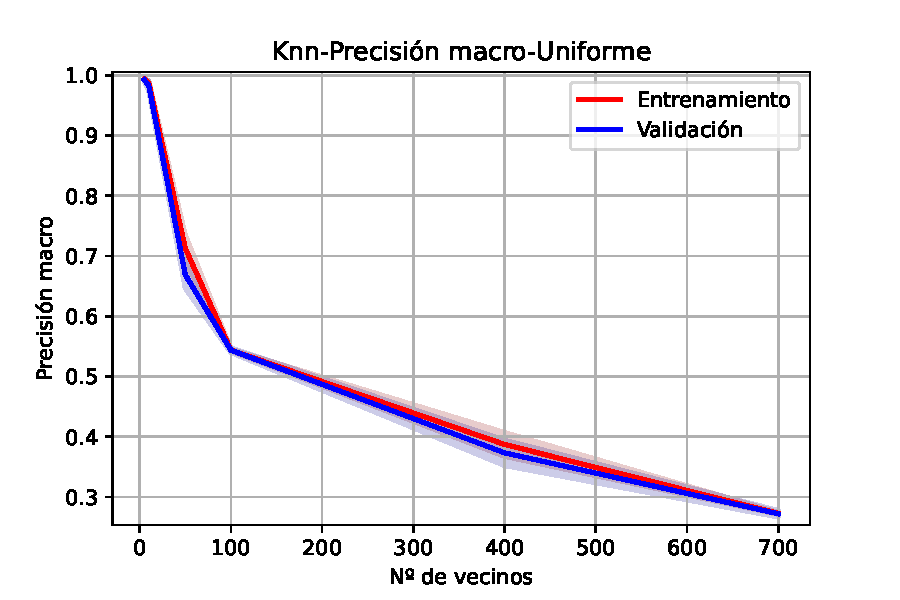
\includegraphics[width=\textwidth]{imagenes/resultados/curvas_validación/Knn-Precisión macro-Uniforme.pdf}
	\caption{Curva de validación para modelo KNN uniforme, Precisión macro}
	\label{fig:res_knn_vc_precision}
\end{figure}

Las tres figuras muestran la independencia del nº de vecinos del clasificador frente a un sobre ajuste y sub ajuste del modelo. También, para siete características, a mayor valores de $n$ peor es el resultado del modelo. 

Los mejores resultados se obtienen para el rango de $\left[5,20\right]$, como se muestra en las siguientes figuras:

\begin{figure}[H]
	\centering
	\captionsetup{justification=centering}
	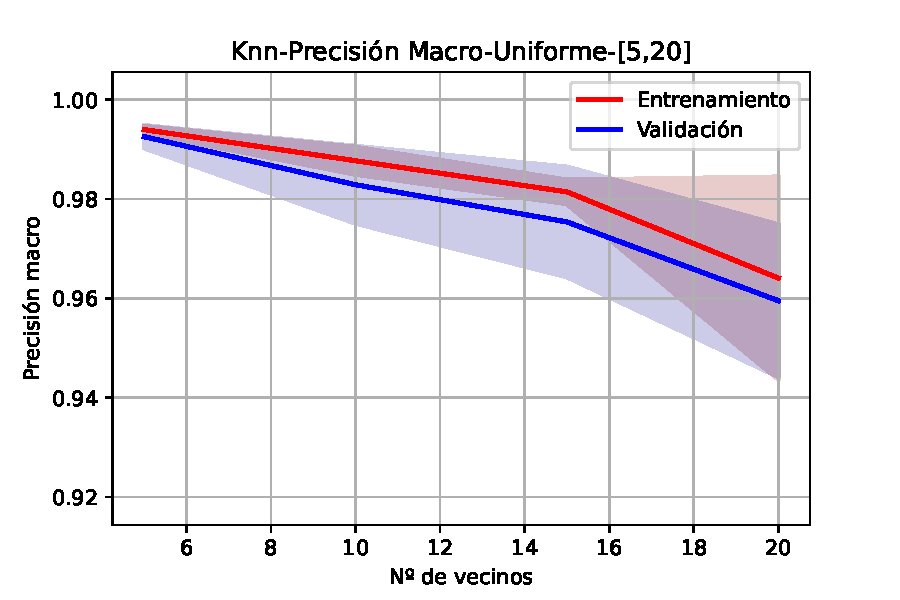
\includegraphics[width=\textwidth]{imagenes/resultados/curvas_validación/Knn-Precisión Macro-Uniforme-[5,20].pdf}
	\caption{Curva de validación para modelo KNN uniforme en rango n=[5,20], Precisión macro}
	\label{fig:res_knn_vc_precision_5,20}
\end{figure}

\begin{figure}[H]
	\centering
	\captionsetup{justification=centering}
	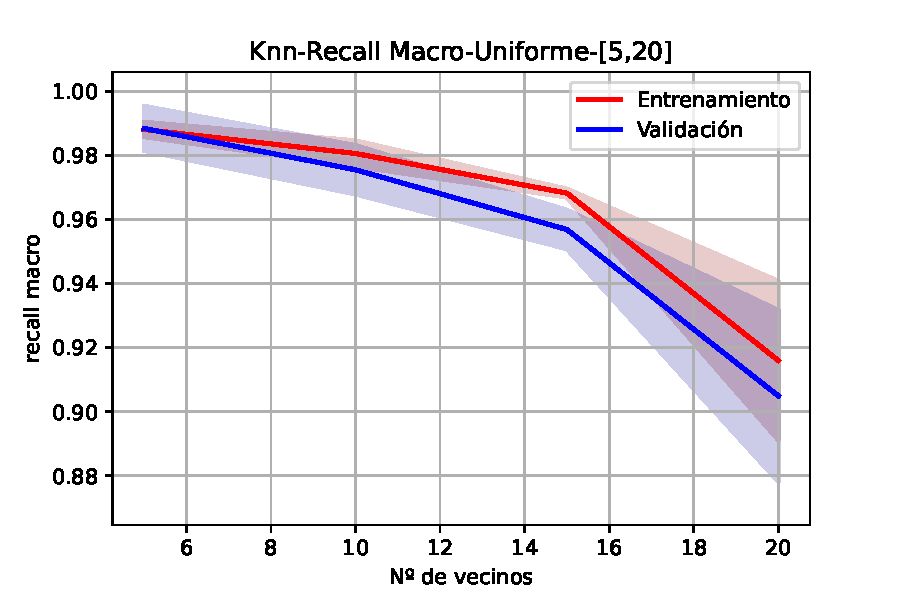
\includegraphics[width=\textwidth]{imagenes/resultados/curvas_validación/Knn-Recall Macro-Uniforme-[5,20].pdf}
	\caption{Curva de validación para modelo KNN uniforme en rango n=[5,20], Recall macro}
	\label{fig:res_knn_vc_recall_5,20}
\end{figure}

\begin{figure}[H]
	\centering
	\captionsetup{justification=centering}
	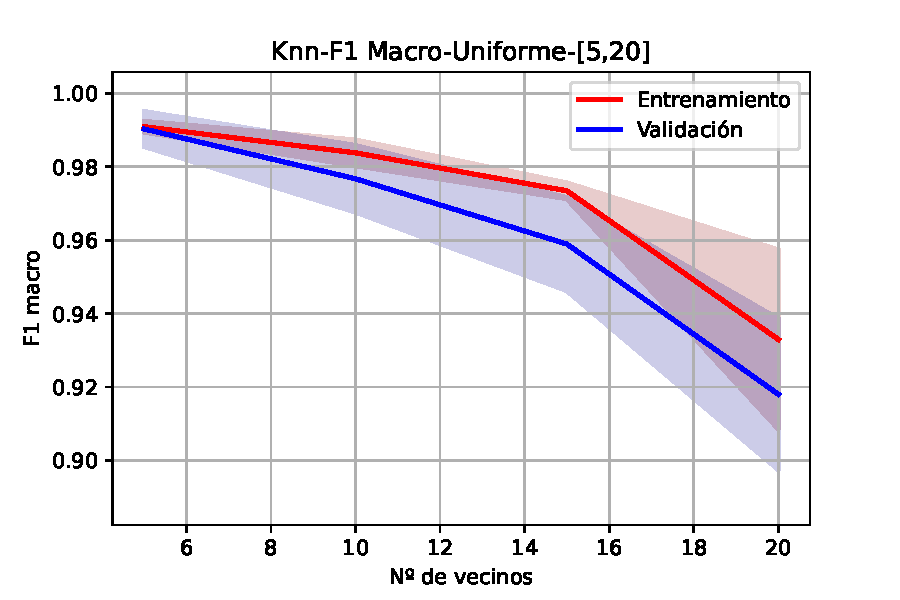
\includegraphics[width=\textwidth]{imagenes/resultados/curvas_validación/Knn-F1 Macro-Uniforme-[5,20].pdf}
	\caption{Curva de validación para modelo KNN uniforme en rango n=[5,20], F1 macro}
	\label{fig:res_knn_vc_f1_5,20}
\end{figure}

En todas las figuras, sobre todo \ref{fig:res_knn_vc_f1_5,20} y \ref{fig:res_knn_vc_recall_5,20}, a partir de $n=15$, inclusive, se presenta un aumento en la desviación de las métricas, indicando una mayor variación en el rendimiento en función de la partición escogida del dataset, lo que representa una menor capacidad de generalización del modelo en la fase de entrenamiento, que no consigue plasmar los mismos buenos resultados (en comparación, porque en general son excelentes, aún con este desliz) en la fase de validación.

De las seis figuras anteriores, se puede afirmar que los mejores resultados, con las siete mejores características, se dan para $n<15$.

\subsubsection{Mejores parámetros B345}

Realizando una búsqueda de parámetros entre $[2,31]$ mejores características y $[5,30]$ vecinos más cercanos, con una estrategia de validación cruzada y mezclado de datos, se obtiene la tabla \ref{res:knn_gs_b345}.

\begin{table}[H]
	\centering
	\captionsetup{justification=centering}
	\begin{tabular}{|c|c|}
		\hline
		Nº de características & 19 \\ \hline
		Nº de vecinos & 6 \\ \hline
	\end{tabular}
	\caption{Mejores parámetros modelo Knn para área B345}
	\label{res:knn_gs_b345}
\end{table}

Los resultados por clase y promediados para un modelo knn de 6 vecinos más cercanos utilizando las 19 mejores características devuelve los resultados de la tabla \ref{res:knn_report_b345}.

\begin{table}[H]
	\centering
	\captionsetup{justification=centering}
	\begin{tabular}{|c|c|c|c|c|}
		\hline
		\multicolumn{5}{|c|}{Métricas por clase} \\ \hline
		Clase & Precisión & Recall & F1 & Nº de muestras \\ \hline \hline
		LX01 & 1.000000 & 0.994845 & 0.997416 & 194 \\ \hline
		TC01 & 0.995643 & 1.000000 & 0.997817 & 457 \\ \hline
		TC02 & 1.000000 & 1.000000 & 1.000000 & 22 \\ \hline
		TC03 & 1.000000 & 1.000000 & 1.000000 & 185 \\ \hline
		TC04 & 1.000000 & 0.960000 & 0.979592 & 25 \\ \hline
		TC05 & 0.984615 & 1.000000 & 0.992248 & 64 \\ \hline
		TC06 & 1.000000 & 1.000000 & 1.000000 & 397 \\ \hline
		TC08 & 1.000000 & 0.933333 & 0.965517 & 15 \\ \hline
		TC10 & 0.972540 & 0.961538 & 0.967008 & 442 \\ \hline
		TC11 & 0.979834 & 0.985680 & 0.982748 & 838 \\ \hline
		TC12 & 0.999778 & 1.000000 & 0.999889 & 4511 \\ \hline
		TC14 & 1.000000 & 0.987805 & 0.993865 & 82 \\ \hline
		TC15 & 0.997590 & 1.000000 & 0.998794 & 414 \\ \hline
		TC17 & 0.996721 & 1.000000 & 0.998358 & 304 \\ \hline
		TC19 & 0.998305 & 0.998305 & 0.998305 & 590 \\ \hline
		TC20 & 0.992424 & 1.000000 & 0.996198 & 131 \\ \hline
		TC23 & 1.000000 & 0.921053 & 0.958904 & 38 \\ \hline
		TC25 & 1.000000 & 1.000000 & 1.000000 & 30 \\ \hline
		TC27 & 1.000000 & 1.000000 & 1.000000 & 21 \\ \hline
		TC29 & 1.000000 & 1.000000 & 1.000000 & 269 \\ \hline
		TC31 & 1.000000 & 1.000000 & 1.000000 & 18 \\ \hline
		TC35 & 1.000000 & 1.000000 & 1.000000 & 52 \\ \hline \hline
		Micro & 0.995934 & 0.995934 & 0.995934 & 9099 \\ \hline
		Macro & 0.952933 & 0.945329 & 0.948985 & 9099 \\ \hline
		Ponderada & 0.995934 & 0.995934 & 0.995920 & 9099 \\ \hline
	\end{tabular}
	\caption{Métricas por clase y promedios para área B345 con modelo Knn}
	\label{res:knn_report_b345}	
\end{table}

\begin{table}[H]	
	\centering
	\captionsetup{justification=centering}
	\begin{tabular}{|c|c|c|c|}
		\hline
		Promedio & Precisión & Recall & F1 \\ \hline
		Micro & 99.59\% & 99.59\% & 99.59\% \\ \hline
		Macro & 95.29\% & 94.53\% & 94.90\% \\ \hline
		Ponderada & 99.59\% & 99.59\% & 99.59\% \\ \hline
	\end{tabular}
	\caption{Métricas promediadas Knn B345}
	\label{res:knn_report_resumen_b345}
\end{table}

La tabla \ref{res:knn_report_resumen_b345} muestra que los resultados promedios para el problema general son muy elevados, obteniéndose un $94.9\%$ para $F_{1}$. La diferencia entre los promediados micro y ponderado frente al macro indican (además de un desbalanceado en los datos) que no todas las clases tienen un rendimiento cerca del $100\%$ como indicarían los otros promedios, la TC23 obtiene un $F_{1} = 95.89\%$ y sólo presenta 38 muestras, por ejemplo. Sin embargo, los resultados son más que satisfactorios dada la poca cantidad de muestras y la gran cantidad de clases (22). Los valores de recall y precisión indican que el modelo es bueno identificando muestras positivas de cada clase y acertando en la identificación de estas a la clase pertinente, respectivamente.

\mynote{Es muy posible que se obtengan resultados diferentes por milésimas seleccionando menos características, ya que el método \textit{GridSearchCV} va a buscar el mejor valor posible según la métrica escogida y devolverá los parámetros de esa métrica, sin considerar que el segundo mejor valor puede estar en el orden de millonésimas por debajo. Sin embargo, con los parámetros escogidos, la clasificación es la mejor posible, así que tampoco importa cuantos coja. Se puede jugar un poco y obtener la métrica para cada combinación de parámetros, pero no es el objetivo de este trabajo, solo decir que para estos parámetros el clasificador funciona que da gusto.}
	
%\subsubsection{Influencia del nº de características en el modelo Knn}
%\begin{table}[H]
%	\resizebox{\textwidth}{!}{
%	\begin{tabular}{|c|c|c|c|c|c|c|c|c|c|c|}
%		\hline
%		k/N & 5 & 6 & 7 & 8 & 9 & 10 & 11 & 12 & 13 & 15 \\ \hline
%		2 & 0.750197 & 0.732362 & 0.731626 & 0.718620 & 0.713603 & 0.706865 & 0.695101 & 0.664370 & 0.649346 & 0.636021 \\ \hline
%		3 & 0.846253 & 0.836495 & 0.842503 & 0.824873 & 0.829736 & 0.820059 & 0.816807 & 0.809634 & 0.804559 & 0.801296 \\ \hline
%		4 & 0.901158 & 0.899806 & 0.895775 & 0.887616 & 0.885607 & 0.879149 & 0.876432 & 0.858412 & 0.854349 & 0.847261 \\ \hline
%		5 & 0.981725 & 0.979560 & 0.972743 & 0.964084 & 0.963459 & 0.956822 & 0.954959 & 0.945003 & 0.945325 & 0.930744 \\ \hline
%		6 & 0.987181 & 0.981166 & 0.973448 & 0.963671 & 0.963409 & 0.956422 & 0.942576 & 0.941990 & 0.939666 & 0.935943 \\ \hline
%		7 & 0.988256 & 0.985800 & 0.981250 & 0.979446 & 0.976043 & 0.973633 & 0.972225 & 0.962696 & 0.958911 & 0.957556 \\ \hline
%		8 & 0.987228 & 0.979825 & 0.979331 & 0.975007 & 0.974665 & 0.969068 & 0.968959 & 0.966239 & 0.966950 & 0.955709 \\ \hline
%		9 & 0.986717 & 0.984970 & 0.984872 & 0.978443 & 0.978988 & 0.971343 & 0.971098 & 0.964389 & 0.964831 & 0.953251 \\ \hline
%		10 & 0.988313 & 0.983662 & 0.984488 & 0.976018 & 0.976452 & 0.974554 & 0.974404 & 0.968801 & 0.969779 & 0.964441 \\ \hline
%		11 & 0.985269 & 0.983850 & 0.984471 & 0.981281 & 0.981639 & 0.977377 & 0.978565 & 0.969286 & 0.969621 & 0.960472 \\ \hline
%		12 & 0.989227 & 0.986803 & 0.986217 & 0.985610 & 0.985447 & 0.982737 & 0.982819 & 0.975377 & 0.974679 & 0.965164 \\ \hline
%		13 & 0.991577 & 0.988773 & 0.987402 & 0.983631 & 0.985323 & 0.978803 & 0.978720 & 0.965096 & 0.966117 & 0.959325 \\ \hline
%		15 & 0.991461 & 0.985820 & 0.985076 & 0.984702 & 0.984453 & 0.982741 & 0.983352 & 0.979010 & 0.978615 & 0.969601 \\ \hline
%	\end{tabular}}
%	\caption{F1 macro para diferentes N\textdegree de vecinos en función del número de mejores características}
%	\label{tab:res_knn_kvsn}
%\end{table}
%
%\mynote{En la tabla \ref{tab:res_knn_kvsn} solo se muestran quince de las treinta y una características pues, además del tamaño considerable de la tabla en la página, a partir de 16 $F_{1}$ sólo aumenta en milésimas. La tabla completa se encuentra en los anexos de resultados.}
%
%En la tabla \ref{tab:res_knn_kvsn}, a partir de 5 características $F_{1}$ se estabiliza, aumentando su valor 1-2 décimas (2-3 para mayores valores de N)
%hasta llegar a las 15 características. Además, según la tabla \ref{tab:res_knn_kvsn_stdev}, a mayor valor de k menor es la desviación de la métrica.
%
%Por tanto, se puede concluir que cualquier valor de $n$ en el rango [5,15) presenta buenos resultados para el área B345.
%
%\begin{table}[H]
%	\resizebox{\textwidth}{!}{
%	\begin{tabular}{|c|c|c|c|c|c|c|c|c|c|c|}
%		\hline
%		k/N & 5 & 6 & 7 & 8 & 9 & 10 & 11 & 12 & 13 & 15 \\ \hline
%		2 & 0.031263 & 0.028918 & 0.027425 & 0.038645 & 0.038485 & 0.033838 & 0.027380 & 0.011099 & 0.011499 & 0.019158 \\ \hline
%		3 & 0.022516 & 0.023287 & 0.021248 & 0.020090 & 0.021299 & 0.014314 & 0.012023 & 0.013558 & 0.016777 & 0.015160 \\ \hline
%		4 & 0.011580 & 0.010484 & 0.013045 & 0.013121 & 0.014088 & 0.018962 & 0.020212 & 0.006876 & 0.011304 & 0.013484 \\ \hline
%		5 & 0.007101 & 0.008787 & 0.015885 & 0.017089 & 0.017825 & 0.018747 & 0.015785 & 0.016174 & 0.016110 & 0.013600 \\ \hline
%		6 & 0.009172 & 0.011432 & 0.008986 & 0.018212 & 0.016982 & 0.017263 & 0.017706 & 0.018679 & 0.015959 & 0.014962 \\ \hline
%		7 & 0.004283 & 0.005415 & 0.007737 & 0.007010 & 0.015303 & 0.013305 & 0.014690 & 0.017637 & 0.015151 & 0.014291 \\ \hline
%		8 & 0.001790 & 0.010028 & 0.010619 & 0.009653 & 0.010005 & 0.011424 & 0.011686 & 0.012188 & 0.012579 & 0.017748 \\ \hline
%		9 & 0.004908 & 0.004796 & 0.004699 & 0.008346 & 0.008339 & 0.008184 & 0.008223 & 0.011039 & 0.010391 & 0.008906 \\ \hline
%		10 & 0.005957 & 0.007101 & 0.007109 & 0.012818 & 0.012815 & 0.013961 & 0.014291 & 0.015866 & 0.016634 & 0.013791 \\ \hline
%		11 & 0.012960 & 0.013744 & 0.013643 & 0.012318 & 0.014393 & 0.013041 & 0.013674 & 0.015642 & 0.015421 & 0.022719 \\ \hline
%		12 & 0.004536 & 0.003496 & 0.003331 & 0.003176 & 0.002955 & 0.002077 & 0.002331 & 0.005933 & 0.007653 & 0.008392 \\ \hline
%		13 & 0.003761 & 0.004431 & 0.004382 & 0.005867 & 0.007458 & 0.008414 & 0.008670 & 0.018212 & 0.018673 & 0.015392 \\ \hline
%		15 & 0.004415 & 0.009609 & 0.009790 & 0.009930 & 0.009757 & 0.011447 & 0.010203 & 0.009231 & 0.009019 & 0.015241 \\ \hline
%	\end{tabular}}
%	\caption{Desviación típica para tabla superior.}
%	\label{tab:res_knn_kvsn_stdev}
%\end{table}
%
%\begin{figure}[H]
%	\centering
%	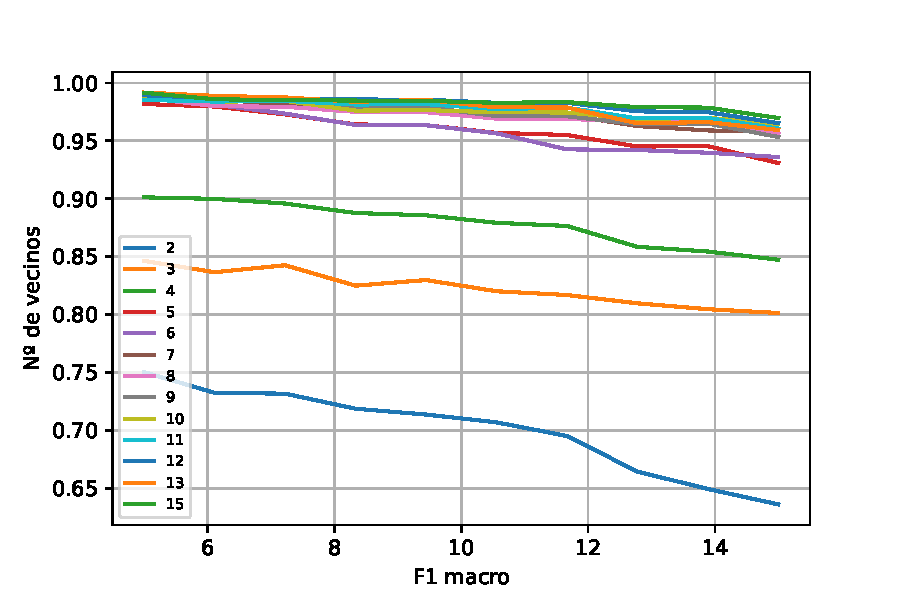
\includegraphics[width=\textwidth]{imagenes/resultados/knn/knn_f1vsn.pdf}
%	\caption{F1 macro en función del nº de vecinos para modelo Knn}
%	\label{res:knn_f1vsn}
%\end{figure}
%
%
%\begin{table}[H]
%	\centering
%	\begin{tabular}{|c|c|c|c|c|}
%		\hline
%		\multicolumn{5}{|c|}{Métricas por clase} \\ \hline
%		Clase & Precisión & Recall & F1 & Nº de muestras \\ \hline \hline
%		LX01 & 0.994792 & 0.984536 & 0.989637 & 194 \\ \hline
%		TC01 & 0.995643 & 1.000000 & 0.997817 & 457 \\ \hline
%		TC02 & 0.956522 & 1.000000 & 0.977778 & 22 \\ \hline
%		TC03 & 1.000000 & 0.994595 & 0.997290 & 185 \\ \hline
%		TC04 & 1.000000 & 0.960000 & 0.979592 & 25 \\ \hline
%		TC05 & 0.984615 & 1.000000 & 0.992248 & 64 \\ \hline
%		TC06 & 1.000000 & 0.997481 & 0.998739 & 397 \\ \hline
%		TC08 & 1.000000 & 1.000000 & 1.000000 & 15 \\ \hline
%		TC10 & 0.909292 & 0.929864 & 0.919463 & 442 \\ \hline
%		TC11 & 0.962740 & 0.955847 & 0.959281 & 838 \\ \hline
%		TC12 & 0.999335 & 1.000000 & 0.999668 & 4511 \\ \hline
%		TC14 & 1.000000 & 0.987805 & 0.993865 & 82 \\ \hline
%		TC15 & 0.997585 & 0.997585 & 0.997585 & 414 \\ \hline
%		TC17 & 0.986928 & 0.993421 & 0.990164 & 304 \\ \hline
%		TC19 & 1.000000 & 0.998305 & 0.999152 & 590 \\ \hline
%		TC20 & 0.992424 & 1.000000 & 0.996198 & 131 \\ \hline
%		TC23 & 1.000000 & 0.921053 & 0.958904 & 38 \\ \hline
%		TC25 & 1.000000 & 0.933333 & 0.965517 & 30 \\ \hline
%		TC27 & 1.000000 & 0.904762 & 0.950000 & 21 \\ \hline
%		TC29 & 0.977695 & 0.977695 & 0.977695 & 269 \\ \hline
%		TC31 & 0.894737 & 0.944444 & 0.918919 & 18 \\ \hline
%		TC35 & 0.941176 & 0.923077 & 0.932039 & 52 \\ \hline \hline
%		Micro & 0.989339 & 0.989339 & 0.989339 & 9099 \\ \hline
%		Macro & 0.938847 & 0.930600 & 0.934415 & 9099 \\ \hline
%		Ponderada & 0.989430 & 0.989339 & 0.989355 & 9099 \\ \hline
%	\end{tabular}
%	\caption{Métricas para clases del área B345, con promedios}
%	\label{res:knn_class_report}
%\end{table}

\subsection{Resultados con clasificador Knn para área C1C9}

\subsubsection{Curvas de validación}

\begin{figure}[H]
	\centering
	\captionsetup{justification=centering}
	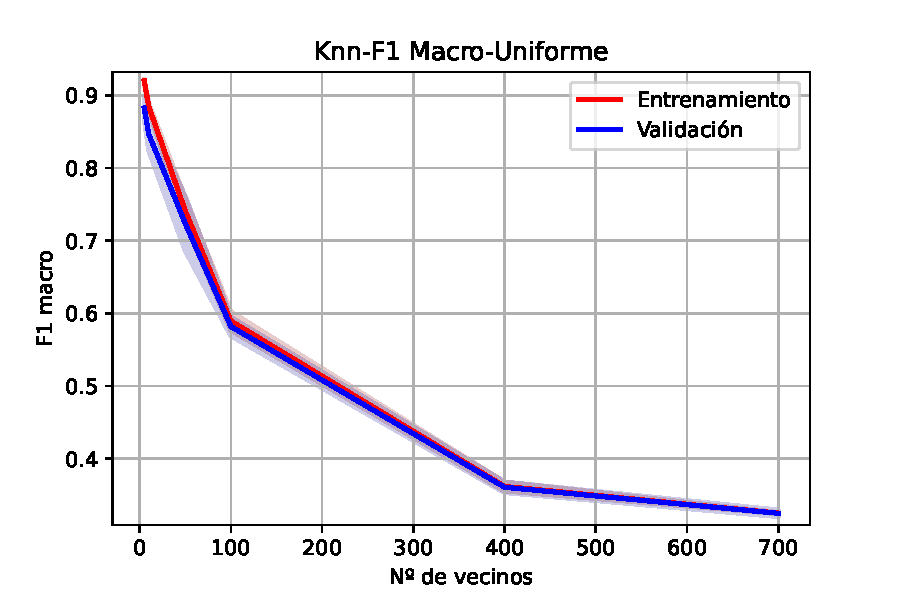
\includegraphics[width=\textwidth]{imagenes/resultados/curvas_validación/Knn-F1 macro-Uniforme-c1c9.pdf}
	\caption{Curva de validación para modelo KNN uniforme, F1 macro}
	\label{fig:res_knn_vc_f1_c1c9}
\end{figure}

\begin{figure}[H]
	\centering
	\captionsetup{justification=centering}
	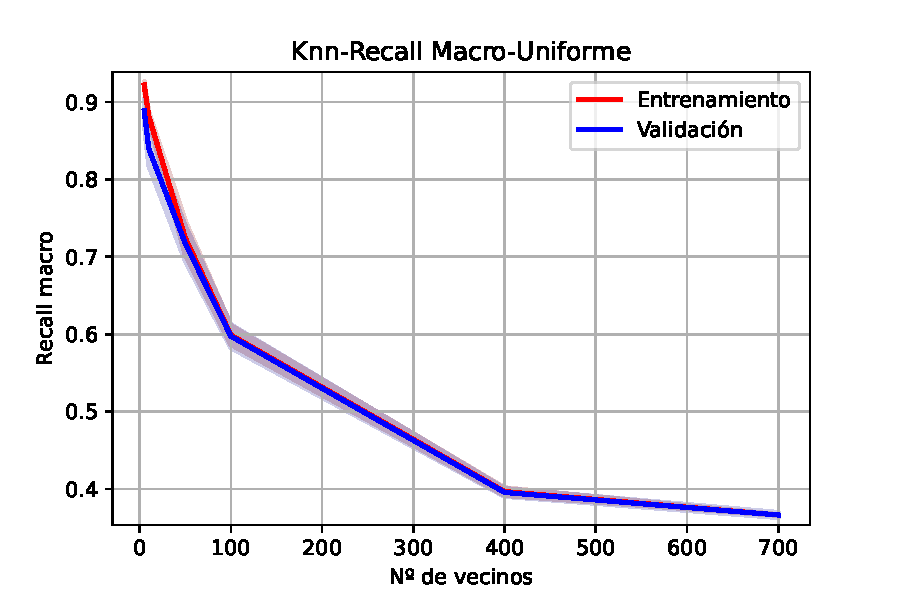
\includegraphics[width=\textwidth]{imagenes/resultados/curvas_validación/Knn-Recall macro-Uniforme-c1c9.pdf}
	\caption{Curva de validación para modelo KNN uniforme, Recall macro}
	\label{fig:res_knn_vc_recall_c1c9}
\end{figure}

\begin{figure}[H]
	\centering
	\captionsetup{justification=centering}
	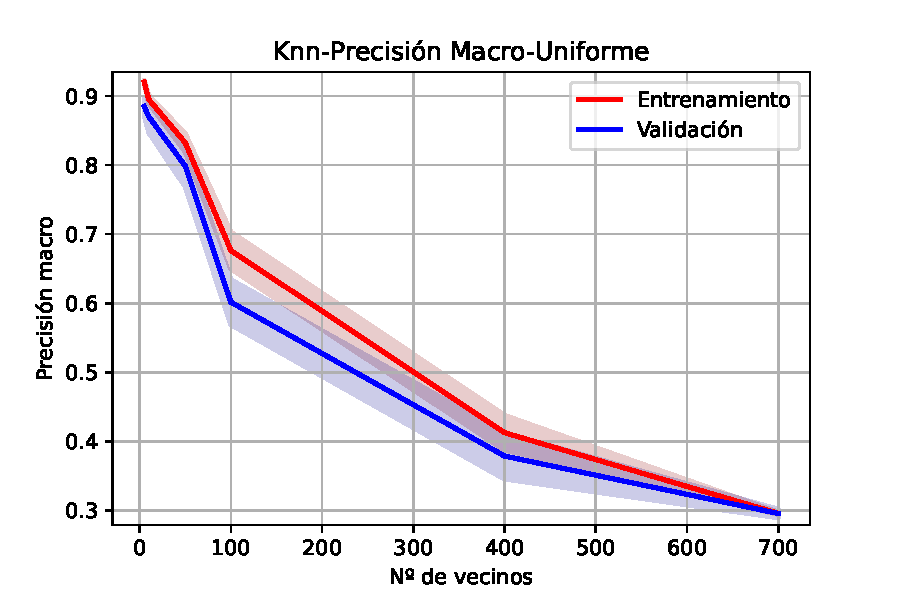
\includegraphics[width=\textwidth]{imagenes/resultados/curvas_validación/Knn-Precisión macro-Uniforme-c1c9.pdf}
	\caption{Curva de validación para modelo KNN uniforme, Precisión macro}
	\label{fig:res_knn_vc_precision_c1c9}
\end{figure}

A diferencia que para el área B345, en este caso la curva de validación para el área C1C9 muestra un resultado sobre ajustado en precisión. Aunque el modelo es exhaustivo encontrando muestras positivas, no consigue acertarlas correctamente. Los falsos positivos para el caso de validación son mayores que en el entrenamiento, indicando que existe una similitud entre varios símbolos que el clasificador no es capaz de discriminar correctamente. Este comportamiento se acentúa en $n=100$, desapareciendo por completo en $n=700$ y, aun así, los resultados son aceptables para $n<30$.

\begin{figure}[H]
	\centering
	\captionsetup{justification=centering}
	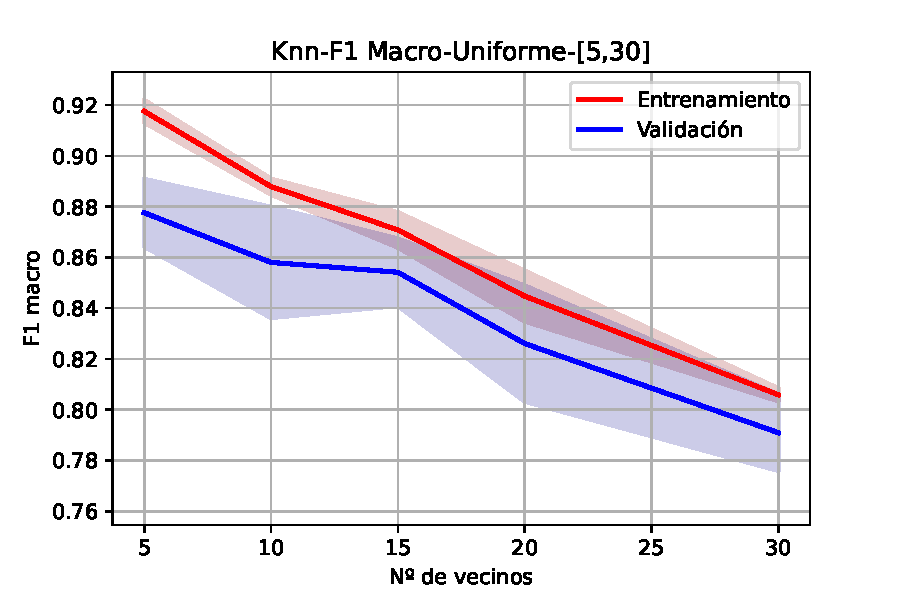
\includegraphics[width=\textwidth]{imagenes/resultados/curvas_validación/Knn-F1 Macro-Uniforme-c1c9[5,30].pdf}
	\caption{Curva de validación para modelo KNN uniforme, F1 macro}
	\label{fig:res_knn_vc_precision_c1c9[5,30]}
\end{figure}

\subsubsection{Mejores parámetros C1C9}

Realizando una búsqueda de parámetros entre $[2,31]$ mejores características y $[5,30]$ vecinos más cercanos, con una estrategia de validación cruzada y mezclado de datos, se obtiene la tabla \ref{res:knn_gs_c1c9}.

\begin{table}[H]
	\centering
	\captionsetup{justification=centering}
	\begin{tabular}{|c|c|}
		\hline
		Nº de características & 7 \\ \hline
		Nº de vecinos & 5 \\ \hline
	\end{tabular}
	\caption{Mejores parámetros modelo Knn para área C1C9}
	\label{res:knn_gs_c1c9}
\end{table}

Los resultados por clase y promediados para un modelo knn de 5 vecinos más cercanos utilizando las 7 mejores características devuelve los resultados de la tabla \ref{res:knn_report_c1c9}.

\begin{table}[H]
	\centering
	\captionsetup{justification=centering}
	\begin{tabular}{|c|c|c|c|c|}
		\hline
		\multicolumn{5}{|c|}{Métricas por clase} \\ \hline
		Clase & Precisión & Recall & F1 & Nº de muestras \\ \hline \hline
		LE06 & 0.794737 & 0.868815 & 0.830126 & 869 \\ \hline
		LE07 & 0.758879 & 0.662316 & 0.707317 & 613 \\ \hline
		LE09a & 0.991525 & 0.991525 & 0.991525 & 354 \\ \hline
		LE10 & 0.917040 & 0.978469 & 0.946759 & 418 \\ \hline
		LE11 & 0.888112 & 0.830065 & 0.858108 & 153 \\ \hline
		LE12 & 0.930061 & 0.960417 & 0.944995 & 1440 \\ \hline
		LE13 & 0.852217 & 0.745690 & 0.795402 & 464 \\ \hline
		MO02 & 0.881890 & 0.903226 & 0.892430 & 124 \\ \hline
		MO05 & 0.992201 & 0.980308 & 0.986219 & 1168 \\ \hline
		MO08 & 0.935185 & 0.870690 & 0.901786 & 116 \\ \hline
		MO10 & 0.956289 & 0.966637 & 0.961435 & 1109 \\ \hline
		MO15 & 0.842105 & 0.914286 & 0.876712 & 35 \\ \hline
		MO17 & 0.969697 & 0.941176 & 0.955224 & 34 \\ \hline
		MO20 & 0.658537 & 0.870968 & 0.750000 & 31 \\ \hline
		MO22 & 0.890756 & 0.837945 & 0.863544 & 253 \\ \hline
		Micro & 0.906559 & 0.906559 & 0.906559 & 7181 \\ \hline
		Macro & 0.576488 & 0.579241 & 0.576591 & 7181 \\ \hline
		Ponderada & 0.906031 & 0.906559 & 0.905327 & 7181 \\ \hline
	\end{tabular}
	\caption{Métricas por clase y promedios para área C1C9 con modelo Knn}
	\label{res:knn_report_c1c9}	
\end{table}

\begin{table}[H]	
	\centering
	\captionsetup{justification=centering}
	\begin{tabular}{|c|c|c|c|}
		\hline
		Promedio & Precisión & Recall & F1 \\ \hline
		Micro & 90.66\% & 90.66\% & 90.66\% \\ \hline
		Macro & 57.65\% & 57.92\% & 57.66\% \\ \hline
		Ponderada & 90.6\% & 90.66\% & 90.53\% \\ \hline
	\end{tabular}
	\caption{Métricas promediadas Knn C1C9}
	\label{res:knn_report_resumen_c1c9}
\end{table}

Las métricas ponderadas de la tabla \ref{res:knn_report_resumen_c1c9} revelan que, en el caso de promedio macro, aun existiendo clases con un alto valor de rendimiento, existen otras cuyos valores no son tal elevados, siendo aquellas menos frecuentes en el dataset. En general los resultados son aceptables, excepto para las clases MO20 y LE07.

\mynote{\textbf{Esto se debe a que la calidad de las imágenes de la C1C9 es bastante peor que la B345, porque en muchas aparecen hasta dedos. No sé si puedo mostrar imágenes ejemplo de los símbolos, pero supongo que si no, al menos puedo hacer un inciso a porqué los resultados salen peor que para la B345}.}

%\subsubsection{Influencia del nº de características en el modelo Knn}
%\begin{table}[H]
%	\resizebox{\textwidth}{!}{
%		\begin{tabular}{|c|c|c|c|c|c|c|c|c|c|c|}
%			\hline
%			k/n & 5 & 6 & 7 & 8 & 9 & 10 & 11 & 12 & 13 & 15 \\ \hline
%			2 & 0.660351 & 0.659113 & 0.649249 & 0.644123 & 0.652822 & 0.639869 & 0.655416 & 0.653679 & 0.637519 & 0.634175 \\ \hline
%			3 & 0.774633 & 0.764143 & 0.761893 & 0.754922 & 0.758031 & 0.754958 & 0.751379 & 0.743985 & 0.744765 & 0.740667 \\ \hline
%			4 & 0.834093 & 0.829328 & 0.829576 & 0.823813 & 0.822685 & 0.811232 & 0.808611 & 0.801191 & 0.805684 & 0.804415 \\ \hline
%			5 & 0.881294 & 0.871179 & 0.871143 & 0.869219 & 0.866350 & 0.866916 & 0.864499 & 0.856663 & 0.857033 & 0.857363 \\ \hline
%			6 & 0.876549 & 0.866209 & 0.872498 & 0.859462 & 0.858577 & 0.852567 & 0.851383 & 0.844738 & 0.847902 & 0.840928 \\ \hline
%			7 & 0.877466 & 0.864204 & 0.872170 & 0.861328 & 0.865580 & 0.858739 & 0.860466 & 0.849003 & 0.850871 & 0.842538 \\ \hline
%			8 & 0.881931 & 0.872454 & 0.878042 & 0.872454 & 0.871443 & 0.862174 & 0.868691 & 0.862320 & 0.863260 & 0.854792 \\ \hline
%			9 & 0.875723 & 0.861127 & 0.872371 & 0.858797 & 0.865442 & 0.852997 & 0.858776 & 0.844760 & 0.845437 & 0.838170 \\ \hline
%			10 & 0.880983 & 0.878961 & 0.872075 & 0.872905 & 0.866851 & 0.861961 & 0.860365 & 0.850296 & 0.847008 & 0.839249 \\ \hline
%			11 & 0.880941 & 0.871367 & 0.871894 & 0.867910 & 0.872122 & 0.862643 & 0.863072 & 0.855191 & 0.859294 & 0.846094 \\ \hline
%			12 & 0.884365 & 0.867537 & 0.873713 & 0.867695 & 0.865381 & 0.853263 & 0.859611 & 0.850419 & 0.852613 & 0.842012 \\ \hline
%			13 & 0.871192 & 0.857921 & 0.866745 & 0.854738 & 0.862419 & 0.853122 & 0.852007 & 0.848010 & 0.846950 & 0.837385 \\ \hline
%			14 & 0.867074 & 0.862574 & 0.868024 & 0.862102 & 0.863141 & 0.849403 & 0.854475 & 0.847440 & 0.848595 & 0.840671 \\ \hline
%			15 & 0.854392 & 0.843811 & 0.843492 & 0.829945 & 0.835355 & 0.809559 & 0.813387 & 0.801150 & 0.804072 & 0.794957 \\ \hline
%			16 & 0.856922 & 0.840174 & 0.847410 & 0.829957 & 0.826216 & 0.812471 & 0.812454 & 0.789768 & 0.807726 & 0.796728 \\ \hline
%			17 & 0.858164 & 0.845579 & 0.846955 & 0.833529 & 0.836478 & 0.818352 & 0.825421 & 0.812664 & 0.813273 & 0.800794 \\ \hline
%			18 & 0.854830 & 0.842250 & 0.838757 & 0.824953 & 0.821445 & 0.805324 & 0.813603 & 0.805735 & 0.802046 & 0.798083 \\ \hline
%			19 & 0.859329 & 0.840790 & 0.847554 & 0.836103 & 0.827789 & 0.811015 & 0.808460 & 0.798256 & 0.810436 & 0.797352 \\ \hline
%			20 & 0.835959 & 0.830450 & 0.833114 & 0.816145 & 0.809001 & 0.799138 & 0.787499 & 0.779040 & 0.775196 & 0.753221 \\ \hline
%			21 & 0.848853 & 0.817713 & 0.825867 & 0.814144 & 0.812350 & 0.804573 & 0.797692 & 0.778039 & 0.775528 & 0.765795 \\ \hline
%			22 & 0.836096 & 0.817077 & 0.824121 & 0.806797 & 0.803234 & 0.790651 & 0.782546 & 0.769489 & 0.761104 & 0.748714 \\ \hline
%			23 & 0.839378 & 0.822893 & 0.822122 & 0.813259 & 0.803920 & 0.789965 & 0.789334 & 0.765730 & 0.762785 & 0.753235 \\ \hline
%			24 & 0.852524 & 0.836858 & 0.834629 & 0.826161 & 0.815779 & 0.789310 & 0.773577 & 0.767940 & 0.764457 & 0.752308 \\ \hline
%			25 & 0.860073 & 0.841441 & 0.844501 & 0.823069 & 0.823015 & 0.805952 & 0.785418 & 0.772661 & 0.768648 & 0.752512 \\ \hline
%			26 & 0.835819 & 0.826877 & 0.823908 & 0.796692 & 0.791323 & 0.786089 & 0.777135 & 0.753200 & 0.742657 & 0.736103 \\ \hline
%			27 & 0.817487 & 0.807374 & 0.790659 & 0.782090 & 0.779622 & 0.763147 & 0.758142 & 0.740285 & 0.734570 & 0.728442 \\ \hline
%			28 & 0.836409 & 0.825019 & 0.820146 & 0.801469 & 0.798138 & 0.777125 & 0.774338 & 0.755973 & 0.752267 & 0.734691 \\ \hline
%			29 & 0.833154 & 0.825340 & 0.817927 & 0.805052 & 0.795270 & 0.779908 & 0.772263 & 0.752701 & 0.748578 & 0.737149 \\ \hline
%			31 & 0.822426 & 0.814392 & 0.818956 & 0.811287 & 0.813079 & 0.801768 & 0.794864 & 0.771089 & 0.756721 & 0.739770 \\ \hline
%	\end{tabular}}
%	\caption{F1 macro para diferentes N\textdegree de vecinos en función del número de mejores características}
%	\label{tab:res_knn_kvsn_c1c9}
%\end{table}

\section{SVM}

Los modelos SVM de \textit{Sklearn} permiten obtener predicciones probabilísticas de los datos de validación, permitiendo el uso de la curva de precisión-recall en la evaluación de su rendimiento.

\subsection{SVM con área C1c9}

\subsubsection{Curvas de validación para diferentes Kernel}

La cuadrícula de imágenes \ref{res:svc_vc} representa las curvas de validación para los diferentes kernel aplicables a un modelo SVM, implementados en la clase SVC de \textit{Sklearn}, definidos en las ecuaciones \ref{eqn:svm_kernel_lineal}, \ref{eqn:svm_kernel_rbf}, \ref{eqn:svm_kernel_poly} y \ref{eqn:svm_kernel_sigmoid}.

\begin{figure}[H]
	\captionsetup{justification=centering}
	\centering
	\begin{subfigure}[b]{.45\linewidth}
		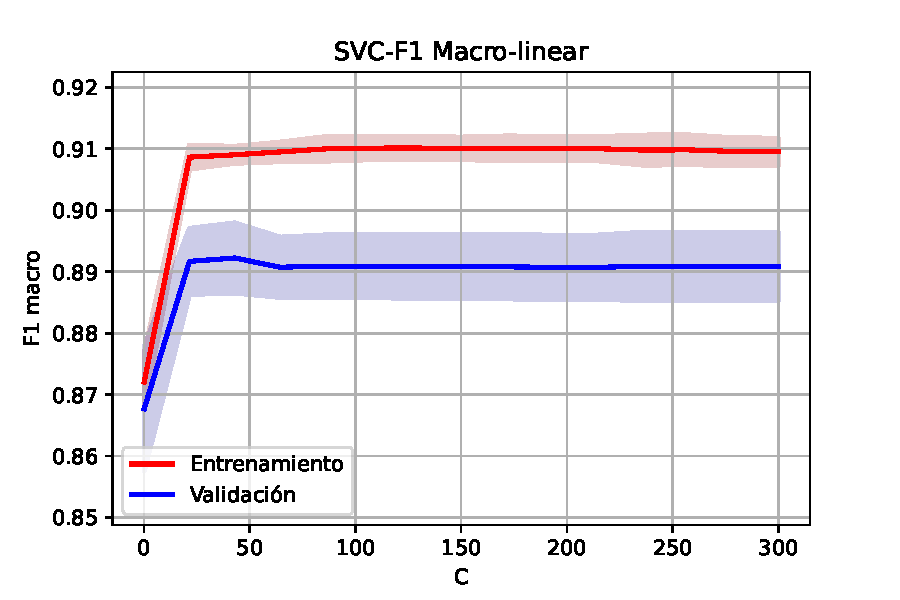
\includegraphics[width=\linewidth]{imagenes/resultados/svm/curvas_validacion/SVC-F1 Macro-linear.pdf}
		\caption{Kernel Lineal}
		\label{res:svc_vc_lineal}
	\end{subfigure}
	\begin{subfigure}[b]{.45\linewidth}
		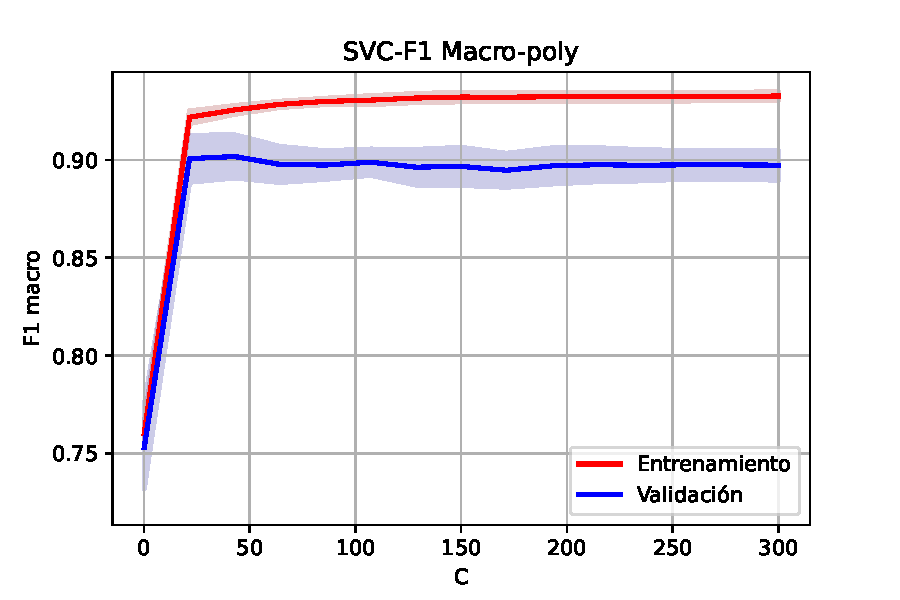
\includegraphics[width=\linewidth]{imagenes/resultados/svm/curvas_validacion/SVC-F1 Macro-poly.pdf}
		\caption{Kernel polinómico}
		\label{res:svc_vc_poly}
	\end{subfigure}
	\begin{subfigure}[b]{.45\linewidth}
		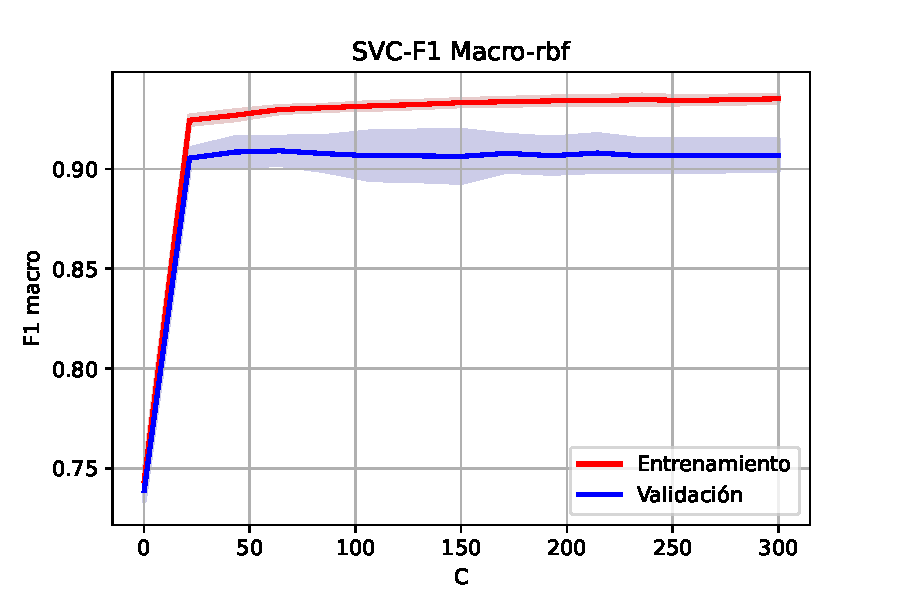
\includegraphics[width=\linewidth]{imagenes/resultados/svm/curvas_validacion/SVC-F1 Macro-rbf.pdf}
		\caption{Kernel RBF}
		\label{res:svc_vc_rbf}
	\end{subfigure}
	\begin{subfigure}[b]{.45\linewidth}
		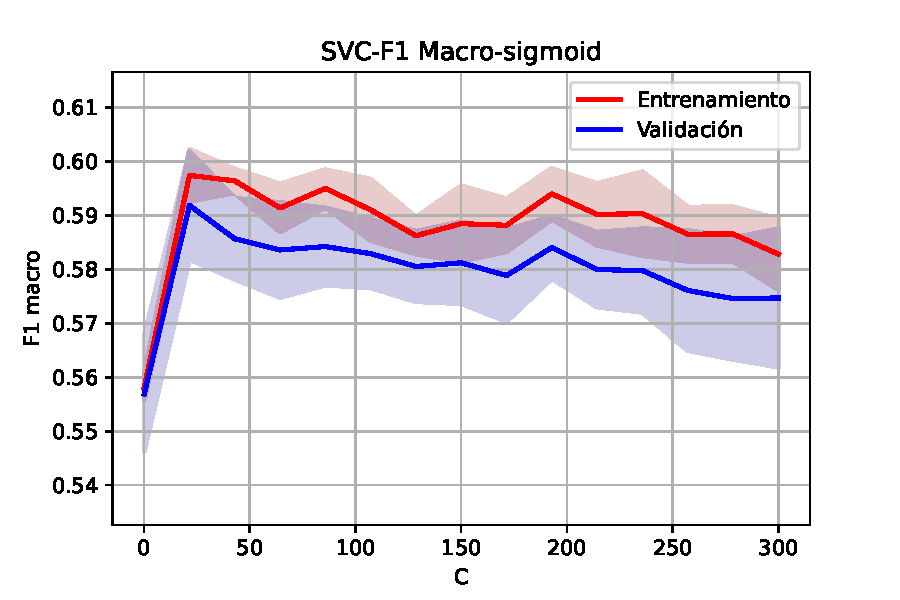
\includegraphics[width=\linewidth]{imagenes/resultados/svm/curvas_validacion/SVC-F1 Macro-sigmoid.pdf}
		\caption{Kernel Sigmoid}
		\label{res:svc_vc_sigmoid}
	\end{subfigure}
	\caption{Curvas de validación para kernels de modelo SVC en área C1c9 en función de parámetro de penalización C.}
	\label{res:svc_vc}
\end{figure}

Para los cuatro kernel disponibles en la clase SVC de \textit{Sklearn}, el modelo presenta para valores altos de C un sobreajuste de los datos de entrenamiento frente a los de validación. Para valores pequeños de C, el modelo tiene un buen comportamiento.

La figura \ref{res:svc_vc_sigmoid} presenta un rendimiento inferior a 0.6, indicando que el kernel \textit{sigmoid} no es aplicable a esta clasificación.

\paragraph{Kernel RBF}

El kernel RBF (ecuación \ref{eqn:svm_kernel_rbf}) depende del parámetro $\gamma$ en su definición. La figura \ref{res:svc_vc_rbf_gamma} representa la curva de validación de dicho parámetro:

\begin{figure}[H]
	\centering
	\captionsetup{justification=centering}
	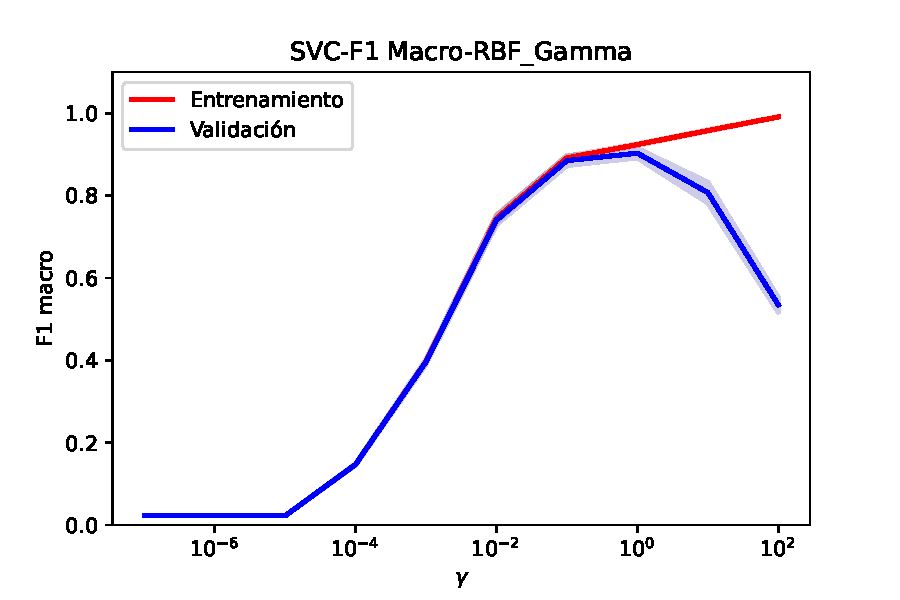
\includegraphics[width=\textwidth]{imagenes/resultados/svm/curvas_validacion/SVC-F1 Macro-RBF_Gamma.pdf}
	\caption{Curva de validación para kernel RBF en función de $\gamma$ en área C1c9.}
	\label{res:svc_vc_rbf_gamma}
\end{figure}

A partir de $\gamma = 10^{-2} = 0.01$ el modelo empieza a sobre ajustar los datos de entrenamiento frente a validación, divergiendo completamente a partir de $\gamma=10^{-1}=0.1$. Para $\gamma<10^{-2}$ el rendimiento para entrenamiento y validación muestran los mismos resultados, indicando que el modelo funciona correctamente para tal rango. Sin embargo, el rendimiento para estos valores es muy bajo.

\paragraph{Kernel polinómico}

Definido por la ecuación \ref{eqn:svm_kernel_poly}, el kernel polinómico es dependiente de parámetros $\gamma$, $r$ (también llamado \textit{coef0}) y $d$ (grado del polinomio, en inglés \textit{degree}).

\begin{figure}[H]
	\captionsetup{justification=centering}
	\centering
	\begin{subfigure}[b]{.45\linewidth}
		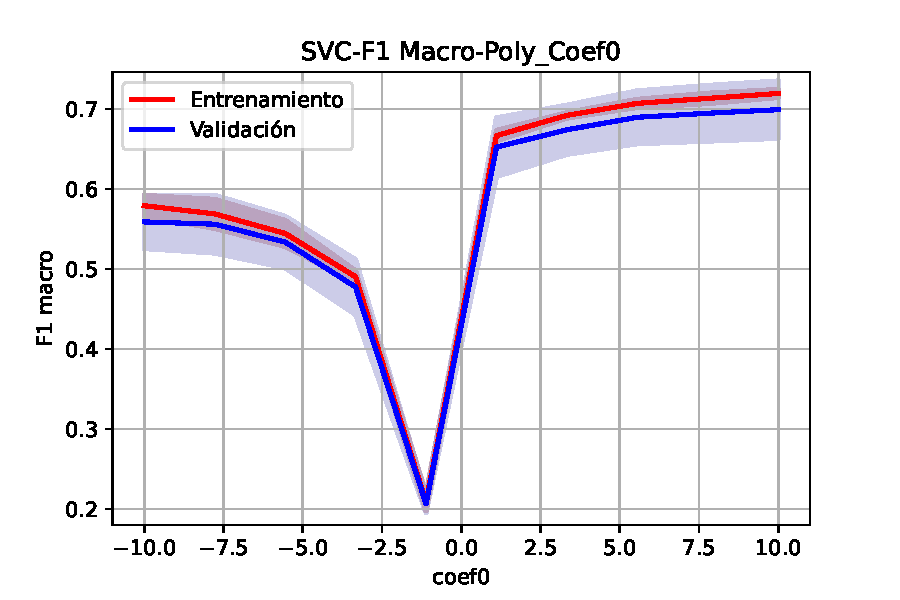
\includegraphics[width=\linewidth]{imagenes/resultados/svm/curvas_validacion/SVC-F1 Macro-Poly_Coef0.pdf}
		\caption{Curva de validación para kernel polinómico en función de $r$ en área C1c9.}
		\label{res:svc_vc_poly_coef0}
	\end{subfigure}
	\begin{subfigure}[b]{.45\linewidth}
		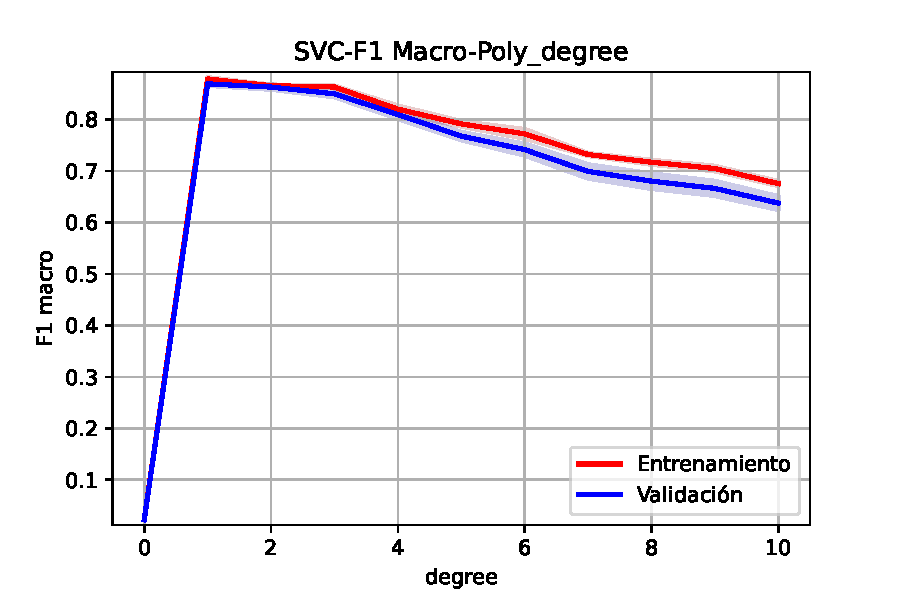
\includegraphics[width=\linewidth]{imagenes/resultados/svm/curvas_validacion/SVC-F1 Macro-Poly_degree.pdf}
		\caption{Curva de validación para kernel polinómico en función del grado en área C1c9.}
		\label{res:svc_vc_poly_degree}
	\end{subfigure}
	\caption{Curvas de validación para kernel polinómico}
	\label{res:svc_vc_poly_kernel}
\end{figure}

La figura \ref{res:svc_vc_poly_coef0} representa un correcto comportamiento del modelo para el rango $r\epsilon[-3,1.75]$, sobre ajustando fuera de estos límites. Para \ref{res:svc_vc_poly_degree}, el modelo funciona correctamente en $d<3$, tendiendo a sobre ajustar a medida que se aumenta el grado del kernel.

\paragraph{Kernel lineal}

El kernel lineal (ecuación \ref{eqn:svm_kernel_lineal}) no requiere de más parámetros excepto $C$, el parámetro de regularización, por lo tanto, su curva de validación ya se haya representada en \ref{res:svc_vc_lineal}.

\subsubsection{Mejores parámetros SVC para área C1C9}

\paragraph{Kernel RBF}

Los mejores parámetros encontrados, según métrica $F_{1}$, para $k\:(\mbox{ANOVA})\:\epsilon\:[2,31]$, $\gamma\:\epsilon\:[10^{-7},10^{2}]$ y $C\:\epsilon\:[1,100]$ han resultado:

\begin{table}[H]
	\begin{tabular}{|c|c|}
		\hline
		Parámetro & Valor \\ \hline
		k (ANOVA) & 9 \\ \hline
		C & 20\\ \hline
		$\gamma$ & 1\\ \hline
	\end{tabular}
\end{table}

\paragraph{Kernel Lineal}

Los mejores parámetros encontrados, según métrica $F_{1}$, para $k\:(\mbox{ANOVA})\:\epsilon\:[2,31]$ y $C\:\epsilon\:[1,100]$ han resultado:

\begin{table}[H]
	\begin{tabular}{|c|c|}
		\hline
		Parámetro & Valor \\ \hline
		k (ANOVA) & 9 \\ \hline
		C & 15\\ \hline
	\end{tabular}
\end{table}

\paragraph{Kernel polinómico}

Los mejores parámetros encontrados, según métrica $F_{1}$, para $k\:(\mbox{ANOVA})\:\epsilon\:[2,31]$ y $C\:\epsilon\:[1,100]$ han resultado:

\begin{table}[H]
	\begin{tabular}{|c|c|}
		\hline
		Parámetro & Valor \\ \hline
		k (ANOVA) & 9 \\ \hline
		C & 15\\ \hline
		r & 1 \\ \hline
		Grado & 3 \\ \hline
		$\gamma$ & 1 \\ \hline
	\end{tabular}
\end{table}

\begin{table}[H]
	\centering
	\captionsetup{justification=centering}
	\resizebox{\columnwidth}{!}{
	\begin{tabular}{|c|c|c|c|}
		\hline
		\multicolumn{2}{|c|}{AUC-Ovo-C1C9-Poly} \\ \hline \hline
		Clase & AUC \\ \hline
		LE06 & 0.897256 \\ \hline
		LE07 & 0.801268 \\ \hline
		LE09a & 1.000000 \\ \hline
		LE10 & 0.982807 \\ \hline
		LE11 & 0.898879 \\ \hline
		LE12 & 0.992003 \\ \hline
		LE13 & 0.943605 \\ \hline
		MO02 & 0.989694 \\ \hline
		MO05 & 0.999336 \\ \hline
		MO08 & 0.982773 \\ \hline
		MO10 & 0.999272 \\ \hline
		MO15 & 0.985674 \\ \hline
		MO17 & 0.988889 \\ \hline
		MO20 & 0.596893 \\ \hline
		MO22 & 0.997976 \\ \hline
	\end{tabular}
	\begin{tabular}{|c|c|}
		\hline
		\multicolumn{2}{|c|}{AUC-Ovo-C1C9-Lineal} \\ \hline \hline
		Clase & AUC \\ \hline
		LE06 & 0.835289 \\ \hline
		LE07 & 0.703032 \\ \hline
		LE09a & 1.000000 \\ \hline
		LE10 & 0.972459 \\ \hline
		LE11 & 0.863337 \\ \hline
		LE12 & 0.924740 \\ \hline
		LE13 & 0.776634 \\ \hline
		MO02 & 0.990316 \\ \hline
		MO05 & 0.999177 \\ \hline
		MO08 & 0.955717 \\ \hline
		MO10 & 0.999730 \\ \hline
		MO15 & 0.966846 \\ \hline
		MO17 & 1.000000 \\ \hline
		MO20 & 0.667409 \\ \hline
		MO22 & 0.996742 \\ \hline
	\end{tabular}
	\begin{tabular}{|c|c|}
		\hline
		\multicolumn{2}{|c|}{AUC-Ovo-C1C9-RBF} \\ \hline \hline
		Clase & AUC \\ \hline
		LE06 & 0.923290 \\ \hline
		LE07 & 0.797598 \\ \hline
		LE09a & 1.000000 \\ \hline
		LE10 & 0.986225 \\ \hline
		LE11 & 0.934888 \\ \hline
		LE12 & 0.990411 \\ \hline
		LE13 & 0.943534 \\ \hline
		MO02 & 0.997832 \\ \hline
		MO05 & 0.998750 \\ \hline
		MO08 & 0.992643 \\ \hline
		MO10 & 0.999781 \\ \hline
		MO15 & 0.993808 \\ \hline
		MO17 & 0.979798 \\ \hline
		MO20 & 0.646762 \\ \hline
		MO22 & 0.997654 \\ \hline
	\end{tabular}}
	\caption{Resultados AUC para diferentes Kernel SVM para área C1C9}
	\label{res:svc_c1c9}
\end{table}

\begin{table}[H]
	\centering
	\captionsetup{justification=centering}
	\begin{tabular}{|c|c|}
		\hline
		Kernel & AUC Macro \\ \hline \hline
		Polinómico & 0.9371 \\ \hline
		Lineal & 0.9116 \\ \hline
		RBF & 0.9467 \\ \hline
	\end{tabular}
	\caption{AUC macro para C1C9}
	\label{res:svc_auc_macro_c1c9}	
\end{table}

\subsection{SVM con área B345}

\subsubsection{Curvas de validación para diferentes Kernel}

La cuadrícula de imágenes \ref{res:svc_vc_b345} representa las curvas de validación para los diferentes kernel aplicables a un modelo SVM, implementados en la clase SVC de \textit{Sklearn}, definidos en las ecuaciones \ref{eqn:svm_kernel_lineal}, \ref{eqn:svm_kernel_rbf}, \ref{eqn:svm_kernel_poly} y \ref{eqn:svm_kernel_sigmoid}.

\begin{figure}[H]
	\captionsetup{justification=centering}
	\centering
	\begin{subfigure}[b]{.45\linewidth}
		\includegraphics[width=\linewidth]{imagenes/resultados/svm/curvas_validacion/b345/SVC-F1 Macro-linear_C.pdf}
		\caption{Kernel Lineal}
		\label{res:svc_vc_lineal_b345}
	\end{subfigure}
	\begin{subfigure}[b]{.45\linewidth}
		\includegraphics[width=\linewidth]{imagenes/resultados/svm/curvas_validacion/b345/SVC-F1 Macro-poly_C.pdf}
		\caption{Kernel polinómico}
		\label{res:svc_vc_poly_b345}
	\end{subfigure}
	\begin{subfigure}[b]{.45\linewidth}
		\includegraphics[width=\linewidth]{imagenes/resultados/svm/curvas_validacion/b345/SVC-F1 Macro-rbf_C.pdf}
		\caption{Kernel RBF}
		\label{res:svc_vc_rbf_b345}
	\end{subfigure}
	\begin{subfigure}[b]{.45\linewidth}
		\includegraphics[width=\linewidth]{imagenes/resultados/svm/curvas_validacion/b345/SVC-F1 Macro-sigmoid_C.pdf}
		\caption{Kernel Sigmoid}
		\label{res:svc_vc_sigmoid_b345}
	\end{subfigure}
	\caption{Curvas de validación para kernels de modelo SVC en área B345 en función de parámetro de penalización C.}
	\label{res:svc_vc_b345}
\end{figure}

Para los cuatro kernel disponibles en la clase SVC de \textit{Sklearn}, en general, el modelo presenta obreajuste de los datos de entrenamiento frente a los de validación. La figura \ref{res:svc_vc_sigmoid} presenta un rendimiento inferior a 0.5, indicando que el kernel \textit{sigmoid} no es aplicable a esta clasificación.

\paragraph{Kernel RBF}

El kernel RBF (ecuación \ref{eqn:svm_kernel_rbf}) depende del parámetro $\gamma$ en su definición. La figura \ref{res:svc_vc_rbf_gamma_b345} representa la curva de validación de dicho parámetro:

\begin{figure}[H]
	\centering
	\captionsetup{justification=centering}
	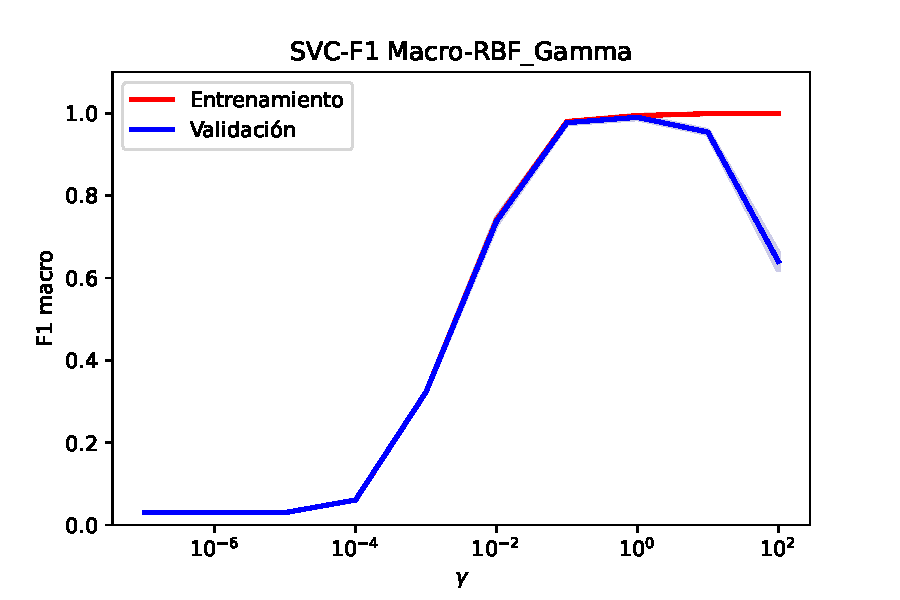
\includegraphics[width=\textwidth]{imagenes/resultados/svm/curvas_validacion/b345/SVC-F1 Macro-RBF_Gamma.pdf}
	\caption{Curva de validación para kernel RBF en función de $\gamma$ en área B345.}
	\label{res:svc_vc_rbf_gamma_b345}
\end{figure}

El modelo presenta un comportamiento perfecto para $\gamma<10^{-1}$, sobre ajustando para valores superiores.

\paragraph{Kernel polinómico}

Definido por la ecuación \ref{eqn:svm_kernel_poly}, el kernel polinómico es dependiente de parámetros $\gamma$, $r$ (también llamado \textit{coef0}) y $d$ (grado del polinomio, en inglés \textit{degree}).

\begin{figure}[H]
	\captionsetup{justification=centering}
	\centering
	\begin{subfigure}[b]{.45\linewidth}
		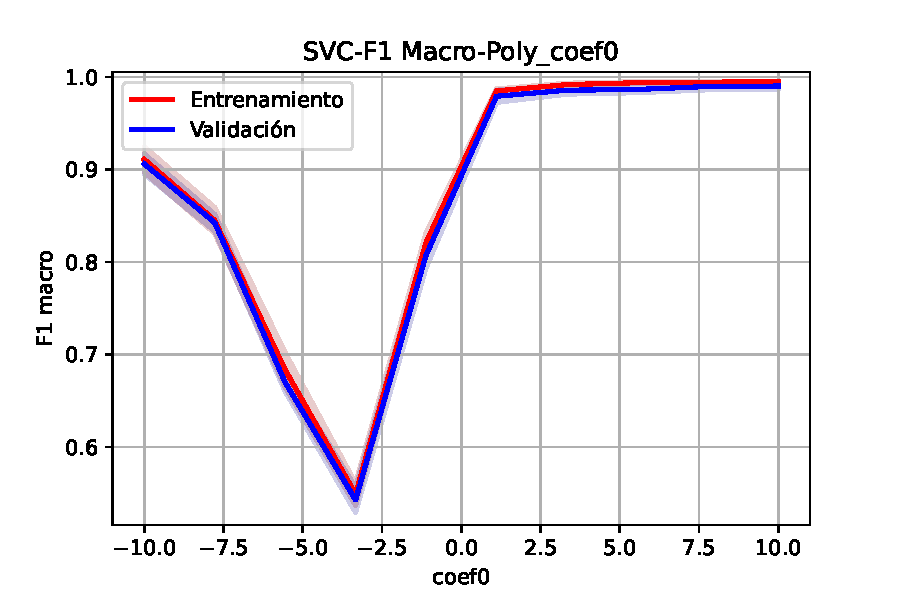
\includegraphics[width=\linewidth]{imagenes/resultados/svm/curvas_validacion/b345/SVC-F1 Macro-Poly_coef0.pdf}
		\caption{Curva de validación para kernel polinómico en función de $r$ en área B345.}
		\label{res:svc_vc_poly_coef0_b345}
	\end{subfigure}
	\begin{subfigure}[b]{.45\linewidth}
		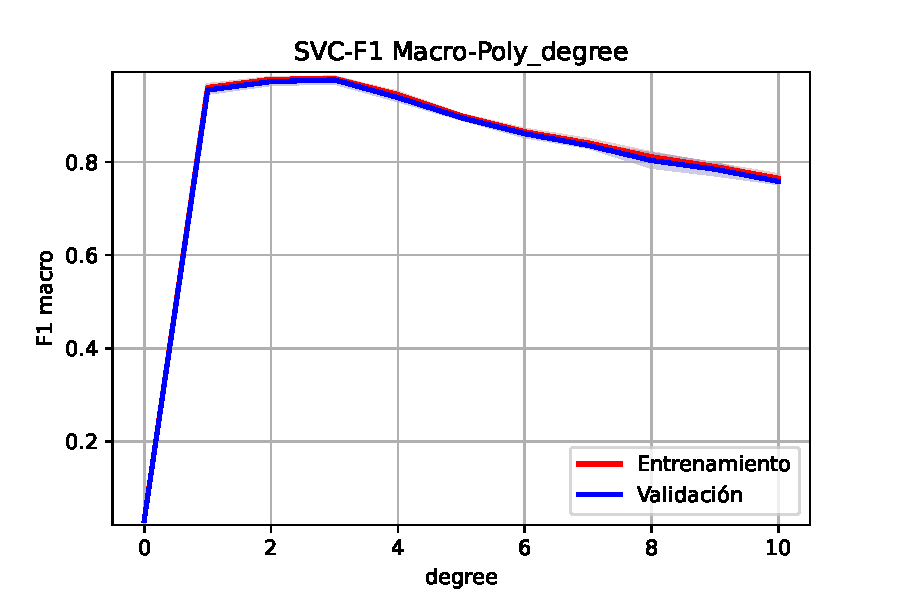
\includegraphics[width=\linewidth]{imagenes/resultados/svm/curvas_validacion/b345/SVC-F1 Macro-Poly_degree.pdf}
		\caption{Curva de validación para kernel polinómico en función del grado en área B345.}
		\label{res:svc_vc_poly_degree_b345}
	\end{subfigure}
	\caption{Curvas de validación para kernel polinómico}
	\label{res:svc_vc_poly_kernel_b345}
\end{figure}

Para el caso del parámetro $r$, el modelo sobre ajusta en casi todo el rango, pero es de tan mínima la diferencia que se puede considerar un comportamiento casi perfecto. En el caso de $d$, el clasificador es impecable pues, ni sobre ajusta ni sub ajusta.

La figura \ref{res:svc_vc_poly_coef0_b345} representa un correcto comportamiento del modelo para el rango $r\epsilon[-3,1.75]$, sobre ajustando fuera de estos límites. Para \ref{res:svc_vc_poly_degree_b345}, el modelo funciona correctamente en $d<3$, tendiendo a sobre ajustar a medida que se aumenta el grado del kernel.

\paragraph{Kernel lineal}

El kernel lineal (ecuación \ref{eqn:svm_kernel_lineal}) no requiere de más parámetros excepto $C$, el parámetro de regularización, por lo tanto, su curva de validación ya se haya representada en \ref{res:svc_vc_lineal_b345}.

\subsubsection{Mejores parámetros SVC para área B345}

\paragraph{Kernel RBF}

Los mejores parámetros encontrados, según métrica $F_{1}$, para $k\:(\mbox{ANOVA})\:\epsilon\:[2,31]$, $\gamma\:\epsilon\:[10^{-7},10^{-1}]$ y $C\:\epsilon\:[1,100]$ han resultado:

\begin{table}[H]
	\begin{tabular}{|c|c|}
		\hline
		Parámetro & Valor \\ \hline
		k (ANOVA) & 12 \\ \hline
		C & 20\\ \hline
		$\gamma$ & 0.1\\ \hline
	\end{tabular}
\end{table}

\paragraph{Kernel Lineal}

Los mejores parámetros encontrados, según métrica $F_{1}$, para $k\:(\mbox{ANOVA})\:\epsilon\:[2,31]$ y $C\:\epsilon\:[1,100]$ han resultado:

\begin{table}[H]
	\begin{tabular}{|c|c|}
		\hline
		Parámetro & Valor \\ \hline
		k (ANOVA) & 12 \\ \hline
		C & 15\\ \hline
	\end{tabular}
\end{table}

\paragraph{Kernel polinómico}

Los mejores parámetros encontrados, según métrica $F_{1}$, para $k\:(\mbox{ANOVA})\:\epsilon\:[2,31]$ y $C\:\epsilon\:[1,100]$ han resultado:

\begin{table}[H]
	\begin{tabular}{|c|c|}
		\hline
		Parámetro & Valor \\ \hline
		k (ANOVA) & 12 \\ \hline
		C & 20\\ \hline
		r & 1 \\ \hline
		Grado & 3 \\ \hline
		$\gamma$ & 1 \\ \hline
	\end{tabular}
\end{table}

\begin{table}[H]
	\centering
	\captionsetup{justification=centering}
	\resizebox{\columnwidth}{!}{
		\begin{tabular}{|c|c|c|c|}
			\hline
			\multicolumn{2}{|c|}{AUC-Ovo-B345-Poly} \\ \hline \hline
			Clase & AUC \\ \hline
			LX01 & 1.000000 \\ \hline
			TC01 & 1.000000 \\ \hline
			TC02 & 1.000000 \\ \hline
			TC03 & 1.000000 \\ \hline
			TC04 & 1.000000 \\ \hline
			TC05 & 1.000000 \\ \hline
			TC06 & 1.000000 \\ \hline
			TC08 & 1.000000 \\ \hline
			TC10 & 0.982638 \\ \hline
			TC11 & 0.996768 \\ \hline
			TC12 & 1.000000 \\ \hline
			TC14 & 1.000000 \\ \hline
			TC15 & 1.000000 \\ \hline
			TC17 & 0.993755 \\ \hline
			TC19 & 1.000000 \\ \hline
			TC20 & 1.000000 \\ \hline
			TC23 & 1.000000 \\ \hline
			TC25 & 1.000000 \\ \hline
			TC27 & 1.000000 \\ \hline
			TC29 & 1.000000 \\ \hline
			TC31 & 1.000000 \\ \hline
			TC35 & 1.000000 \\ \hline
		\end{tabular}
		\begin{tabular}{|c|c|}
			\hline
			\multicolumn{2}{|c|}{AUC-Ovo-B345-Lineal} \\ \hline \hline
			Clase & AUC \\ \hline
			LX01 & 1.000000 \\ \hline
			TC01 & 1.000000 \\ \hline
			TC02 & 1.000000 \\ \hline
			TC03 & 1.000000 \\ \hline
			TC04 & 1.000000 \\ \hline
			TC05 & 1.000000 \\ \hline
			TC06 & 1.000000 \\ \hline
			TC08 & 1.000000 \\ \hline
			TC10 & 0.765972 \\ \hline
			TC11 & 0.963289 \\ \hline
			TC12 & 1.000000 \\ \hline
			TC14 & 1.000000 \\ \hline
			TC15 & 1.000000 \\ \hline
			TC17 & 0.999905 \\ \hline
			TC19 & 1.000000 \\ \hline
			TC20 & 1.000000 \\ \hline
			TC23 & 1.000000 \\ \hline
			TC25 & 1.000000 \\ \hline
			TC27 & 1.000000 \\ \hline
			TC29 & 1.000000 \\ \hline
			TC31 & 1.000000 \\ \hline
			TC35 & 1.000000 \\ \hline
		\end{tabular}
		\begin{tabular}{|c|c|}
			\hline
			\multicolumn{2}{|c|}{AUC-Ovo-B345-RBF} \\ \hline \hline
			Clase & AUC \\ \hline
			LX01 & 1.000000 \\ \hline
			TC01 & 1.000000 \\ \hline
			TC02 & 1.000000 \\ \hline
			TC03 & 1.000000 \\ \hline
			TC04 & 1.000000 \\ \hline
			TC05 & 1.000000 \\ \hline
			TC06 & 1.000000 \\ \hline
			TC08 & 1.000000 \\ \hline
			TC10 & 0.971630 \\ \hline
			TC11 & 0.993925 \\ \hline
			TC12 & 1.000000 \\ \hline
			TC14 & 1.000000 \\ \hline
			TC15 & 1.000000 \\ \hline
			TC17 & 0.999905 \\ \hline
			TC19 & 1.000000 \\ \hline
			TC20 & 1.000000 \\ \hline
			TC23 & 1.000000 \\ \hline
			TC25 & 1.000000 \\ \hline
			TC27 & 1.000000 \\ \hline
			TC29 & 1.000000 \\ \hline
			TC31 & 1.000000 \\ \hline
			TC35 & 1.000000 \\ \hline
	\end{tabular}}
	\caption{Resultados AUC para diferentes Kernel SVM para área B345}
	\label{res:svc_b345}
\end{table}

\begin{table}[H]
	\centering
	\captionsetup{justification=centering}
	\begin{tabular}{|c|c|}
		\hline
		Kernel & AUC Macro \\ \hline \hline
		Polinómico & 0.9988 \\ \hline
		Lineal & 0.9877 \\ \hline
		RBF & 0.9984 \\ \hline
	\end{tabular}
	\caption{AUC macro para B345}
	\label{res:svc_auc_macro_b345}	
\end{table}




\include{doc/discusion_resultados.tex}

\include{doc/impacto_socio_economico.tex}

\chapter{Cronograma de actividades}

\begin{sidewaysfigure}[H]
	\centering
	\captionsetup{justification=centering}
	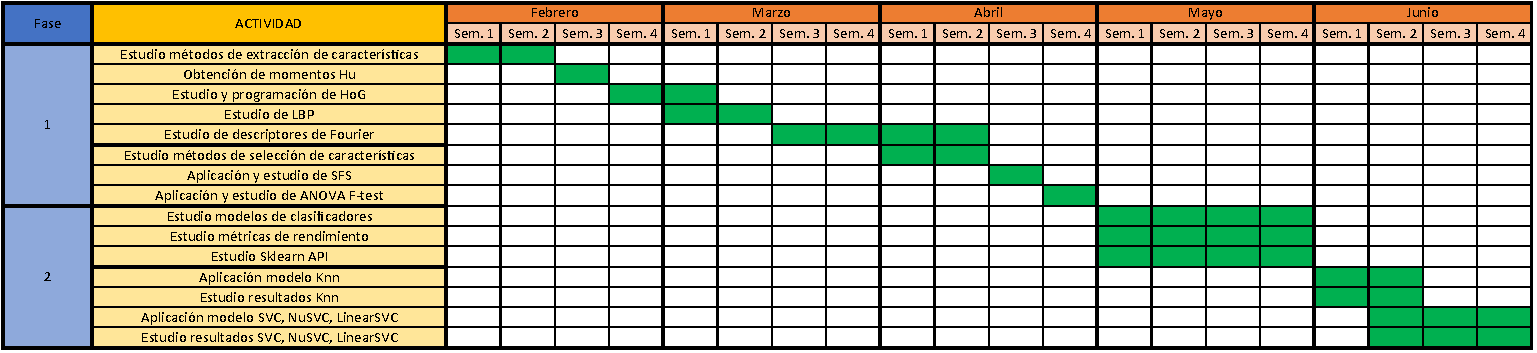
\includegraphics[scale=0.9]{imagenes/cronograma/crono2.pdf}
	\caption{Procesos en la fase de extracción y selección de características}
	\label{crono:crono}
\end{sidewaysfigure}


\include{doc/conclusiones.tex}

\include{doc/futuras_lineas_trabajo.tex}

\clearpage

%----------
%	BIBLIOGRAFÍA
%----------	

%\nocite{*} % Si quieres que aparezcan en la bibliografía todos los documentos que la componen (también los que no estén citados en el texto) descomenta está lína


\clearpage
\addcontentsline{toc}{chapter}{Bibliografía}
\setquotestyle[english]{british} % Cambiamos el tipo de cita porque en el estilo IEEE se usan las comillas inglesas.
\printbibliography


%----------
%	ANEXOS
%----------	

% Si tu trabajo incluye anexos, puedes descomentar las siguientes líneas
%\chapter* {Anexo x}
%\pagenumbering{gobble} % Las páginas de los anexos no se numeran





\end{document}